\documentclass[a4paper,oneside,14pt]{extbook} % -*- coding: vietnamese-utf8 mode: latex -*-
\usepackage[utf8]{vietnam}
\renewcommand{\rmdefault}{utm}
\renewcommand{\sfdefault}{uhv}
\renewcommand{\ttdefault}{ucr}

\usepackage[hmargin={3cm,2cm}]{geometry}
\usepackage{graphicx}
\usepackage{amsmath}
\usepackage[vietnam]{minitoc}
\usepackage{tabularx}
\usepackage{footnote}
\usepackage{tipa}
%\usepackage{fancyvrb}
%\usepackage{subfigure}
%\usepackage{longtable}

%\usepackage{theorem}
%\theoremstyle{break}
%\newtheorem{algo}{Thuật toán}

\setlength{\parskip}{1.2ex plus 0.7ex minus 0.6ex}

\setcounter{minitocdepth}{4}

%\usepackage{tocloft}
%\newcommand{\listalgo}{Danh sách thuật toán}
%\newlistof{algo}{algo}{\listalgo}
\usepackage{float} % fancy floats
\floatstyle{boxed}
\newfloat{algo}{htbp}{loa}[chapter]
\floatname{algo}{Thuật toán}

\usepackage{varioref}
\def\reftextfaceafter{ở trang kế tiếp}
\def\reftextfacebefore{ở trang đối diện}
\def\reftextafter{ở trang kế tiếp}
\def\reftextbefore{ở trang trước}
\def\reftextcurrent{ở trang này}
\def\reftextfaraway#1{ở trang~\pageref{#1}}
\def\reftextpagerange#1#2{ở các trang~\pageref{#1}--\pageref{#2}}%
\def\reftextlabelrange#1#2{\ref{#1} đến~\ref{#2}}%

\newcommand{\note}[1]{\underline{#1}}
\newcommand{\comment}[1]{}

\title{Chương trình bắt lỗi chính tả tiếng Việt}
\author{Nguyễn Thái Ngọc Duy\\0012020}

\begin{document}
\dominitoc
%\doparttoc
\maketitle
%\large

\begin{titlepage}
  \begin{center}
    \Large Lời cảm ơn
  \end{center}
  Xin chân thành cảm ơn TS. Đinh Điền đã tận tình hướng dẫn, giúp đỡ
  trong quá trình làm luận văn. Ngoài ra xin cảm ơn các thành viên
  trong nhóm VCL đã hỗ trợ, động viên hoàn thành luận văn này.
\vskip 1cm
\begin{flushright}
  Nguyễn Thái Ngọc Duy
\end{flushright}
\end{titlepage}

\tableofcontents

%% \chapter{Giới thiệu}
%% \label{cha:intro}
%% \begin{center}

%% I kept the right ones out

%% And let the wrong ones in

%% Had an angel of mercy

%% To see me through all my sins

%% There were times in my life

%% When I was goin' insane

%% Tryin' to walk through the pain

%% ****

%% And when I lost my grip

%% And I hit the floor

%% Yeah, I thought I could leave

%% But couldn't get out the door

%% I was so sick n' tired

%% Of livin' a lie

%% I was wishing that I would die

%% ****

%% It's amazing

%% With the blink of an eye

%% You finally see the light

%% It's amazing

%% That when the moment arrives

%% You know you'll be alright

%% It's amazing

%% And I'm saying a prayer

%% To the desperate hearts tonight


%% ****


%% That one last shot's a Permanent Vacation

%% And a how high can you fly with broken wings

%% Life's a journey - not a destination

%% And I just can't tell just what tomorrow brings


%% ****


%% You have to learn to crawl

%% Before you learn to walk

%% But I just couldn't listen

%% To all that righteous talk

%% I was out on the street

%% Just tryin' to survive

%% Scratchin' to stay alive


%% ****


%% ``To all of you people out there

%% Wherever you are - remember:

%% The light at the end of the tunnel

%% May be you - goodnight''
%%\end{center}

\chapter{Tổng quan}
\label{cha:overview}
\minitoc


Ngôn ngữ là một phần quan trọng của đời sống, là phương tiện chuyển
tải thông tin trong đời sống. Trong thời đại bùng nổ thông tin hiện
nay thì ngôn ngữ đóng vai trò hết sức quan trọng, đặc biệt là ngôn ngữ
viết. 

% Tại sao lại làm đề tài này? (Đặt vấn đề)
Khi viết, đôi khi ta mắc phải những lỗi sai chính tả. Chữ quốc ngữ
chịu ảnh hưởng mạnh của ngôn ngữ nói. Một số âm tiết lại rất dễ 
lầm lẫn, khó phân biệt rõ ràng. Ngôn ngữ nói ở những vùng khác nhau lại
có những dị biệt riêng. Những dị biệt này rất dễ gây ra
những lỗi chính tả khi viết nếu người viết không hiểu rõ về tiếng
Việt.

Những thao tác chuyển thông tin ở dạng khác thành văn bản cũng có thể
gây ra lỗi chính tả. Ví dụ, nếu nhập liệu không cẩn thận dẫn đến lỗi
sai chính tả. Khi ghi lại lời nói của người khác mà người đó sử dụng
giọng địa phương cũng có thể dẫn đến lỗi chính tả. Quét các văn bản
giấy thành văn bản điện tử, sử dụng chương trình nhận dạng chữ, cũng
có thể dẫn đến lỗi chính tả do chương trình nhận dạng nhầm lẫn~\ldots{}

Văn bản dễ bị sai chính tả do nhiều yếu tố khách quan. Để kiểm lỗi
chính tả những văn bản này đòi hỏi nhiều công sức và thời gian, đặc
biệt khi khối lượng văn bản bùng nổ như hiện nay. Do đó cần có một
công cụ hỗ trợ kiểm lỗi chính tả, giúp nhanh chóng phát hiện lỗi chính
tả và đề nghị cách khắc phục.

Trong thời đại tin học hoá, máy tính được tận dụng để giảm thiểu công
sức của con người, đồng thời tăng tính hiệu quả. Tin học đã được áp
dụng trong nhiều lĩnh vực khác nhau và chứng tỏ tính hiệu quả của
nó. Tuy nhiên, việc ứng dụng tin học nhằm hỗ trợ bắt lỗi
chính tả tiếng Việt chỉ mới được bắt đầu trong thời gian gần
đây. Những ứng dụng bắt lỗi chính tả hiện có vẫn còn khá đơn
giản, chưa đáp ứng được nhu cầu thực tế. Luận văn này đề ra một giải
pháp khác để bắt lỗi chính tả, với hy vọng góp phần nâng cao chất
lượng ứng dụng bắt lỗi chính tả tiếng Việt bằng máy tính.

\section{Nội dung bài toán}

Bài toán có thể được phát biểu như sau:
Cho một văn bản tiếng Việt. Tìm tất cả các từ sai chính tả trong văn bản
và đề nghị cách giải quyết lỗi nếu có.

% Phạm vi bài toán

Do ngôn ngữ là một lĩnh vực quá rộng. Việc bắt lỗi chính tả tiếng Việt
tổng quát là cực kỳ khó khăn. Do vậy đề tài này chỉ giới hạn bắt lỗi
chính tả trong các văn bản hành chính.

Chỉ sử dụng từ điển từ, từ điển tiếng và ngữ liệu thô làm đầu vào.

Khái niệm từ ở đây là ``từ từ điển'' --- tức là các từ đơn, từ ghép,
cụm từ được lưu trong từ điển. 

Lỗi chính tả ở đây bao gồm chủ yếu hai loại lỗi sau:
\begin{itemize}
\item Lỗi nhập liệu sai: lỗi gõ thiếu chữ, gõ dư chữ, gõ nhầm vị trí
  hai chữ liên tiếp nhau, gõ nhầm một chữ bằng một chữ khác, sai sót
  do bộ gõ tiếng Việt~\ldots{}
\item Lỗi phát âm sai: chủ yếu là do đặc điểm phát âm của từng vùng,
  dẫn đến sai chính tả khi viết.
\end{itemize}

Không xử lý lỗi từ vựng, lỗi cú pháp.

Giả định rằng, nếu từ bị sai chính tả, thì chỉ sai bởi một trong những
lý do nêu trên {\em một lần}. Nghĩa là không xét những trường hợp sai
chính tả, vừa gõ nhầm chữ này bằng chữ khác, vừa gõ dư chữ.

Giả định người dùng chỉ sử dụng một trong hai cách gõ tiếng Việt là
VNI hoặc TELEX.

Văn bản tiếng Việt được coi là thuần Việt. Không kiểm tra chính tả đối
với những từ nước ngoài. Những từ nước ngoài và các ký hiệu khác đều
bị coi là sai chính tả. 

\section{Đặc điểm}

Bắt lỗi chính tả, xét từ quan điểm tin học, là một bài toán khó. Khó
bởi vì ngôn ngữ là một phần rất quan trọng của đời sống xã hội, nó bao
hàm rất nhiều khía cạnh của văn hoá, xã hội. Ngôn ngữ dùng để diễn đạt
suy nghĩ, chuyển tải thông tin, nên nó chứa đựng một khối lượng tri
thức đồ sộ. Để xử lý ngôn ngữ tự nhiên một cách đúng đắn đòi hỏi một
trình độ nhất định. Bởi vậy, việc giải quyết bài toán bắt lỗi chính tả
bằng máy tính là hết sức khó khăn.

Bắt lỗi chính tả đôi khi được mở rộng để phát hiện những lỗi khác
trong văn bản như lỗi cú pháp, lỗi từ vựng~\ldots{} Điều này cũng dễ
hiểu vì người sử dụng cần một chương trình giúp họ phát hiện và loại
bỏ tất cả các lỗi trong văn bản, không quan trọng lỗi đó thuộc loại
lỗi nào. Thông thường những lỗi từ vựng thường bị nhầm lẫn với lỗi
chính tả, buộc chương trình bắt lỗi chính tả phải phát hiện cả lỗi từ
vựng. Đây là một vấn đề khó vì để bắt lỗi từ vựng, đôi khi cần phải
hiểu nội dung cả văn bản.

Nếu tìm hiểu sâu hơn về bài toán này, ta lại gặp một khó khăn khác do
bản chất của tiếng Việt. Đối với tiếng Việt, cũng như một số
ngôn ngữ châu Á khác, một từ chính tả có thể không tương ứng với một
``từ'' trên văn bản. Đối với các thứ tiếng châu Âu, ta có thể dễ dàng
nhận ra một từ, do các từ được phân cách bằng khoảng trắng. Điều đó
không đúng với tiếng Việt. Trong tiếng Việt, các tiếng được phân cách
bởi khoảng trắng, không phải các từ. Điều này dẫn đến một bài toán
mới: tách từ trong tiếng Việt. Do tiếng Việt là ngôn ngữ nói sao viết
vậy, nên rất ít khi gặp lỗi sai về tiếng. Đa số các lỗi chính tả là
lỗi sai từ, nên việc xác định đâu là từ cực kỳ quan trọng.

Vấn đề càng trở nên khó khăn hơn khi phải thực hiện cùng lúc hai bài
toán là tách từ tiếng Việt và kiểm tra chính tả. Thật sự là tách từ
tiếng Việt trước, sau đó bắt lỗi chính tả. Tuy nhiên, do khi tách từ
thường ngầm định là dữ liệu đúng chính xác. Nên khi phải tách từ trước
bước kiểm tra chính tả, ngầm định trên không còn đúng. Bài toán tách
từ trở thành một bài toán khác, phức tạp hơn.

Do tài nguyên ngữ liệu tiếng Việt, đặc biệt là ngữ liệu tiếng Việt
trên máy tính vẫn còn hạn chế, đề tài này chỉ sử dụng các cách hình
thành lỗi chính tả, từ điển từ tiếng Việt và ngữ liệu văn bản dạng
thô. Việc không thể áp dụng được những thông tin cấp cao hơn như từ
loại, cú pháp, ngữ nghĩa~\ldots{} sẽ làm hạn chế đáng kể khả năng của
chương trình.

%% Dùng sai từ là lỗi từ vựng

\section{Hướng giải quyết}

% Bối cảnh %%%%Nổ thêm về bối cảnh ở đây. Cố để lấn qua trang kế%%%

Bài toán bắt lỗi chính tả đã được tìm hiểu từ rất lâu. Tuy nhiên đa số
đều tập trung vào các ngôn ngữ phổ dụng ở châu Âu. Trong khi đó các ngôn
ngữ châu Á, đặc biệt là tiếng Việt, có những đặc trưng riêng, đặt ra
nhiều thách thức mới. Bài toán bắt lỗi chính tả trên các ngôn ngữ châu
Á như tiếng Trung Quốc, tiếng Hàn Quốc, tiếng Nhật, tiếng Thái và tiếng Việt
chỉ bắt đầu được nghiên cứu gần đây.

Đối với các ngôn ngữ châu Âu, cách giải quyết đơn giản là dựa vào từ
điển. Nếu một từ trên văn bản không có trong từ điển nghĩa là từ đó
sai chính tả.

Đối với các ngôn ngữ như tiếng Trung Quốc, tiếng Nhật~\ldots{}, nhiều
giải pháp được đề ra để giải quyết bài toán. Tuy nhiên hầu hết các
giải pháp đều dựa trên ý tưởng áp dụng tập nhầm lẫn để phát sinh các
từ gần đúng, sau đó sử dụng mô hình ngôn ngữ để định lượng, xác định
xem từ nào là đúng nhất.


Đề tài này áp dụng cách giải quyết truyền thống, so sánh từ dựa trên
từ điển. Nếu từ không có trong từ điển nghĩa là sai chính tả, từ đó
đưa ra những gợi ý thích hợp.

Bài toán đặt ra một bái toán con khác là tách từ tiếng Việt trong điều
kiện văn bản bị sai chính tả. Cách giải quyết bài toán này là phát sinh
mọi cách tách từ có thể, sử dụng tập nhầm lẫn, và sau đó áp dụng mô hình
ngôn ngữ để tìm ra cách tách từ đúng nhất. Tập nhầm lẫn được phát sinh
dựa vào nguồn gốc gây lỗi. Các lỗi về phát âm sẽ dựa trên các thói
quen phát âm của từng vùng để tạo tập nhầm lẫn. Các lỗi về nhập liệu
sẽ dựa trên các nghiên cứu về lỗi nhập liệu để đưa ra tập nhầm lẫn
tương ứng.


\section{Bố cục luận văn}

Luận văn được chia thành các chương sau:
\begin{itemize}
\item Chương 1 giới thiệu chung về luận văn, các vấn đề cần giải
  quyết, đặc điểm, phạm vi của bài toán và hướng giải quyết.
\item Chương 2 trình bày cơ sở lý thuyết ngôn ngữ học.
\item Chương 3 trình bày cơ sở lý thuyết toán học/tin học. Các mô hình
  được áp dụng để giải quyết bài toán.
\item Chương 4 trình bày mô hình đề nghị cho bắt lỗi chính tả tiếng Việt.
\item Chương 5 trình bày các chi tiết khi cài đặt chương trình.
\item Chương 6 tóm tắt luận văn, các kết quả đạt được, tìm hiểu các
  đặc điểm của mô hình   cũng như chương trình cài đặt, các hạn chế và
  các hướng giải quyết   trong tương lai.
\item Phần phụ lục trình bày các thông tin liên quan.
\end{itemize}

\chapter{Cơ sở lý thuyết ngôn ngữ}
\label{cha:vietnamese}
\minitoc


\section{Âm tiết}

Ngôn ngữ là một hệ thống tín hiệu. Khi nói, vỏ vật chất của tín hiệu
là âm thanh, khi viết nó được thể hiện bằng chữ. Không phải chữ viết
lúc nào cũng phản ánh chính xác các âm tố tương ứng. Vì vậy, các âm tố
được biểu diễn bằng những ký hiệu đặc biệt, gọi là phiên âm. Các ký
hiệu phiên âm thường đặt giữa \textipa{/\quad/} hoặc
\textipa{[\quad]}.

Âm thanh trong tự nhiên được tạo thành nhờ sự rung động của một vật
thể đàn hồi. Âm thanh của tiếng nói được hình thành nhờ ``bộ máy phát
âm'' của con người --- bao gồm môi, răng, lưỡi, khoang miệng, khoang
mũi, yết hầu, thanh hầu, phổi~\ldots{}. Ngoài ra, tai người chỉ có thể
tiếp nhận một khoảng âm thanh nhất định. Những chấn động không nghe
được gọi là siêu âm và âm ngoại.

Âm học phân biệt các âm thanh theo những đặc trưng khác nhau, bao gồm:
độ cao, độ mạnh, độ dài. Độ cao phụ thuộc vào tần số dao động. Tần số
dao động càng lớn thì âm thanh càng cao. Tai người có khả năng nhận
biết độ cao trong khoảng từ 16 đến 20.000 $H_z$. Độ mạnh~(cường độ)
phụ thuộc vào biên độ dao động. Biên độ càng lớn, âm thanh càng
to. Cường độ âm thanh trong ngôn ngữ đảm bảo sự xác minh trong giao tế
và là cơ sở để tạo thành các kiểu trọng âm khác nhau. Độ dài~(trường
độ) là khoảng thời gian kéo dài của âm thanh. Ngôn ngữ chỉ quan trọng
thời gian tương đối của âm thanh. Ví dụ, các nguyên âm có trọng âm
thường dài hơn nguyên âm không có trọng âm.


\subsection{Nguyên âm và phụ âm}

Các âm tố có thể chia thành nguyên âm và phụ âm, dựa vào các đặc điểm
âm học, cấu âm và vai trò trong cấu tạo âm tiết.

Nguyên âm có đặc điểm cấu tạo:
\begin{itemize}
\item Luồng hơi ra tự do, không bị cản trở, không có vị trí cấu âm.
\item Bộ máy phát âm căng thẳng toàn bộ.
\item Luồng hơi ra yếu.
\end{itemize}

Phụ âm có đặc điểm cấu tạo hoàn toàn trái ngược với nguyên âm:
\begin{itemize}
\item Luồng hơi bị cản trở do sự xuất hiện chướng ngại trên lối ra của
  luồng không khí, chướng ngại thường xuất hiện ở các khoang trên
  thanh hầu do các khí quan tiếp xúc nhau hay nhích gần nhau mà thành,
  điểm có chướng ngại được gọi là vị trí cấu âm của phụ âm.
\item Bộ máy phát âm không căng thẳng toàn bộ mà sự căng thẳng cơ thịt
  tập trung ở vị trí cấu âm.
\item Luồng hơi ra mạnh.
\end{itemize}

Nguyên âm và phụ âm có chức năng khác nhau trong cấu tạo âm tiết. Các
nguyên âm thường làm hạt nhân hay đỉnh của âm tiết, còn phụ âm thường
là yếu tố đi kèm, không tạo thành âm tiết~(trừ các âm phụ vang).

Những âm tố có đặc tính giống nguyên âm nhưng thường chỉ đi kèm, bản
thân không tạo thành âm tiết được gọi là {\em bán nguyên âm}. Ví dụ,
các âm tố viết là u, i trong các âm ``sau'', ``mai'' trong tiếng Việt.


\subsection{Âm vị}

Âm vị là đơn vị nhỏ nhất của cơ cấu âm thanh ngôn ngữ, dùng để cấu tạo
và phân biệt hình thức ngữ âm của những đơn vị có nghĩa của ngôn ngữ
--- từ và hình vị. Ví dụ, các từ ``tôi'' và ``đôi'', ``ta'' và ``đa''
được phân biệt bởi các âm vị \textipa{/t/} và \textipa{/d/}.

Âm vị là đơn vị nhỏ nhất, vì về mặt tuyến tính nó không thể phân chia
nhỏ hơn nữa. Nếu thay âm vị này bằng âm vị khác trong cùng một bối
cảnh ngữ âm sẽ làm cho từ thay đổi nghĩa hoặc mất nghĩa. Ví dụ, thay
âm \textipa{/t/} trong từ ``toàn'' bằng âm \textipa{/h/} sẽ được
``hoàn'' có nghĩa khác, hoặc nếu thay bằng âm \textipa{/n/} sẽ được
``noàn'' hoàn toàn vô nghĩa.

Âm vị có thể được so sánh như những viên gạch trong việc xây dựng mỗi
ngôn ngữ. Các viên gạch thường giống nhau, nhưng các âm vị về nguyên
tắc phải khác nhau, ít nhất ở một đặc trưng nào đó. Sự khác biệt này
tạo ra khác biệt về hình thức âm thanh của hình vị và từ, tạo ra tín
hiệu khác biệt đối với sự thụ cảm của con người. Vậy âm vị có hai chức
năng cơ bản là {\em chức năng khu biệt}~(vỏ âm thanh của hình vị và
từ) và {\em chức năng cấu tạo}~(chất liệu để cấu tạo nên
những thành tố của những đơn vị có nghĩa).


\subsection{Âm tiết}

Chuỗi lời nói của con người được chia ra làm những khúc đoạn khác
nhau, từ lớn đến nhỏ. Âm tiết là đơn vị phát âm nhỏ nhất, được phân
định tự nhiên trong lời nói con người.

Về phương diện phát âm, dù lời nói chậm đến đâu cũng chỉ phân chia đến
giới hạn của âm tiết mà thôi. Nhưng về phương diện thính giác thì âm
tiết là một tổ hợp âm thanh, có thể gồm nhiều âm tố hoặc đôi khi chỉ
có một âm tố. Mỗi âm tiết chỉ có một âm tố âm tiết tính~(có khả năng
tạo thành âm tiết), còn lại là những yếu tố đi kèm, không tự mình tạo
thành âm tiết. Âm tố âm tiết tính thường được phân bố ở đỉnh hay ở
trung tâm, làm hạt nhân âm tiết, thường là các nguyên âm. Các phụ âm
thường là các yếu tố đi kèm, đứng ngoài biên, hay ở ranh giới của âm
tiết. Đôi khi âm tiết chỉ gồm một nguyên âm.

Trong một số trường hợp, âm tiết có thể có hai hoặc ba nguyên âm. Tuy
nhiên trong số đó chỉ có một nguyên âm tạo đỉnh, các âm tố khác không
tạo thành âm tiết, gọi là bán nguyên âm.

Âm tiết có một số chức năng sau:
\begin{itemize}
\item Âm tiết có chức năng tổ chức chất liệu âm thanh của ngôn ngữ
  bằng cách hợp nhất các âm tố trong một đơn vị phát âm nhỏ nhất.
\item Âm tiết là môi trường để hiện thực hoá các hiện tượng ngôn điệu
  như trọng âm, âm điệu.
\item Âm tiết có chức năng cấu thành tiết điệu của lời nói~\ldots{} Chức
  năng này thể hiện rõ trong ngôn ngữ thơ.
\end{itemize}

Trong các ngôn ngữ âm tiết tính như tiếng Trung Quốc, tiếng Miến Điện,
tiếng Việt~\ldots{} nói chung âm tiết trùng với hình vị --- đơn vị cơ
bản của ngữ pháp. Âm tiết có chức năng là vỏ ngữ âm của hình vị, tạo
nên một đơn vị đặc biệt, gọi là {\em hình tiết}.

Tính chất âm tiết của tiếng Việt đưa đến nhiều hệ quả quan trọng về
ngữ âm cũng như về ngữ pháp. Về mặt ngữ âm, do mỗi âm tiết là vỏ ngữ
âm của một hình vị, và cũng thường là vỏ ngữ âm của từ đơn, nên số
lượng các âm tiết là hữu hạn\footnote{Theo Nguyễn Phan Cảnh ``tiếng
  Việt đưa ra hơn 17.000 âm tiết --- tín hiệu với tự cách là vỏ ngữ âm
khả năng, và chỉ sử dụng hơn 6.900 với tư cách là các âm tiết tồn tại
thực'' (Nguyễn Phan Cảnh, ``Bản chất cấu trúc âm tiết tính của ngôn
ngữ: Dẫn luận vào một miêu tả không phân lập đối với âm vị học Việt
Nam, tạp chí ngôn ngữ, H. 1978, số 2)}.

Là vỏ ngữ âm của một hình vị hay một từ đơn, mỗi âm tiết Tiếng Việt
bao giờ cũng tương ứng với một ý nghĩa nhất định, nên việc phá vỡ cấu
trúc âm tiết trong ngữ lưu, tức xê dịch vị trí các âm tố (âm vị) của
cùng một hình vị từ âm tiết này sang âm tiết khác, là điều ít xảy
ra. Kết quả là trong tiếng Việt, âm tiết có một cấu trúc chặt chẽ, mỗi
âm tố (âm vị) có một vị trí nhất định trong âm tiết. Đứng đầu âm tiết
bao giờ cũng là một phụ âm, cuối âm tiết là một phụ âm hoặc một bán
nguyên âm. Phụ âm cuối luôn luôn ở cuối âm tiết, không thể trở thành
âm đầu được. Do đó, phụ âm cuối và âm đầu làm thành hai đối hệ khác
nhau, có vị trí và chức năng khác nhau trong cấu trúc âm tiết.

Một đặc điểm khác của âm tiết tiếng Việt là mỗi âm tiết đều mang
một thanh điệu nhất định. Việc thể hiện thanh điệu đòi hỏi âm tiết
phải có một trường độ cố định. Tính chất này làm cho các yếu tố bên
trong âm tiết, trừ phụ âm đầu, không có một trường độ cố định, mà đắp
đổi lẫn nhau, liên quan với nhau rất chặt chẽ.


\subsubsection{Cấu trúc âm tiết tiếng Việt}

Trên bình diện ngữ âm học, các cứ liệu thực nghiệm cho thấy âm tiết
Tiếng Việt được cấu tạo bởi ba thành tố độc lập là thanh điệu, phụ âm
đầu và phần còn lại.

Thanh điệu là yếu tố luôn có mặt trong mọi âm tiết tiếng Việt. Tính
chất độc lập về mặt ngữ âm của thanh điệu thể hiện ở chỗ nó có đường
nét và trường độ tương đối ổn định tùy thuộc vào các loại hình âm
tiết.

Phụ âm đầu là yếu tố mở đầu của âm tiết. Tính chất độc lập của phụ âm
đầu thể hiện ở chỗ nó không tham gia vào việc đắp đổi về trường độ
giữa các yếu tố bên trong âm tiết.

Phần còn lại của âm tiết có từ một đến ba yếu tố, gồm một bán nguyên
âm chiếm vị trí trung gian giữa phụ âm đầu và phần còn lại, một nguyên
âm âm tiết tính và một phụ âm hoặc bán nguyên âm cuối, có vai trò kết
thúc âm tiết. Trừ bán nguyên âm trước nguyên âm tiết tính, các yếu tố
của phần còn lại liên kết với nhau rất chặt chẽ, làm thành một
khối. Để đảm bảo cho tính chất cố định về trường độ của âm tiết, các
yếu tố của phần còn lại có sự đắp đổi nhau về trường độ: nếu nguyên âm
dài thì phụ âm hay bán âm cuối ngắn, ngược lại nếu nguyên âm ngắn thì
âm cuối dài. Các yếu tố của phần còn lại không có một trường độ cố
định, và do đó mức độ độc lập về mặt ngữ âm của chúng thấp hơn so với
phụ âm mở đầu âm tiết. Phần còn lại của âm tiết được gọi là phần vần,
vì đây là bộ phận đoạn tính kết hợp với thanh điệu tạo nên vần thơ.

Tóm lại, các yếu tố của âm tiết tiếng Việt có mức độ độc lập khác
nhau, chia làm hai bậc:

\begin{itemize}
\item Bậc một là những yếu tố độc lập về mặt ngữ âm và có thể được
  tách rời về mặt hình thái học. Đó là thanh điệu, âm đầu và vần.
\item Bậc hai là các yếu tố của phần vần, gồm bán nguyên âm trước
  nguyên âm âm tiết tính (được gọi là âm đệm), nguyên âm âm tiết tính
  (được gọi là âm chính), phụ âm hoặc bán nguyên âm cuối (được gọi là
  âm cuối). Các yếu tố này gắn liền với nhau về mặt ngữ âm do tính
  chất cố định về trường độ của âm tiết và chỉ được tách ra bằng những
  ranh giới thuần túy ngữ âm học.
\end{itemize}

Các thành tố của âm tiết tiếng Việt và quan hệ hai bậc giữa các thành
tố được trình bày trong hình~\vref{fig:cautrucamtiet}.

\begin{figure}[htbp]
  \centering
  \begin{tabular}{|c|c|c|c|}
    \hline
    \multicolumn{4}{|c|}{Thanh điệu}\\\hline
    Âm đầu&\multicolumn{3}{c|}{Vần}\\\cline{2-4}
    &Âm đệm&Âm chính&Âm cuối\\\hline
  \end{tabular}
  \caption{Cấu trúc âm tiết}
  \label{fig:cautrucamtiet}
\end{figure}

%\subsection{Các hiện tượng liên quan đến âm tiết}


%\subsubsection{Nguyên âm đôi}


% Sự biến hoá ngữ âm

Khái niệm âm tiết liên quan mật thiết đến sự biến hoá ngữ âm. Vì các
âm tố lời nói không phát âm đơn lập mà được phát âm trong dòng lời nói
liên tục, cho nên các âm tố có thể ảnh hưởng lẫn nhau, đặc biệt là
những âm tố lân cận được phát âm trong cùng một âm tiết, hoặc ở những
âm tiết đi liền nhau. Một số hiện tượng biến hoá ngữ âm thường gặp
trong tiếng Việt:
\begin{itemize}
\item Sự thích nghi. Xuất hiện giữa phụ âm và nguyên âm đứng cạnh
  nhau. Nếu âm tố sau biến đổi cho giống âm tố đi trước, đó là thích
  nghi xuôi. Nếu âm tố trước biến đổi cho hợp với âm tố sau là thích
  nghi ngược. Trong tiếng Việt, nguyên âm và phụ âm cuối kết hợp với
  nhau rất chặt chẽ, tạo thành vần của âm tiết. Hiện tượng thích nghi
  biểu hiện rõ rệt trong những vần có nguyên âm dòng trước và dòng sau
  tròn môi kết hợp với phụ âm cuối ``ng'' và ``c''.
\item Sự đồng hoá (một yếu tố thay đổi để giống yếu tố kia). Ví dụ,
  ``vỏn vẹn'' và ``vẻn vẹn''.
\item Sự dị hoá (hiện tượng rút gọn cho dễ phát âm). Ví dụ, ``ba mươi
  mốt'' và ``băm mốt''.
\end{itemize}

\subsection{Phụ âm đầu}

Phụ âm đầu luôn gắn liền với vị trí và chức năng mở đầu âm tiết. Đi
sau âm đầu trong âm tiết là bán nguyên âm không thành âm tiết (hay còn
gọi là âm đệm).

Hệ thống phụ âm đầu tiếng Việt với số lưỡng đối lập âm vị học tối đa
được thể hiện trên chữ viết. Riêng những âm tiết như ``ăn'',
``uống''~\ldots{} tuy không ghi phụ âm đầu, nhưng thực tế vẫn tồn tại
phụ âm đầu (âm tắt thanh hầu \textipa{/P/}). Trong từng phương ngữ,
một số đối lập có trên chữ viết có thể bị mất đi hoặc bị thay thế. Ví
dụ, trong tiếng Hà Nội không còn đối lập các phụ âm đầu giữa
ch--tr,x--s và gi,d với r. Trong tiếng miền Nam, \textipa{/v/} và
\textipa{/z/} được thay bằng \textipa{/j/}.

Hiện nay, hệ thống phụ âm đầu được sử dụng thực tế trong nhà trường và
trên các văn bản, chung cho các phương ngữ, là hệ thống phụ âm đầu
hình thành trên cơ sở phát âm Hà Nội với sự phân biệt các phụ âm
ch--tr, x--s, g,gi--r gồm 22 phụ âm sau: \textipa{/b, m, f, v, t,
  t\super{h}, d, n, s, z, l, \:t, \:s, \:z, c, \textltailn, k, N, x,
  G, P, h/}\footnote{Phụ âm \textipa{/p/} gặp trong từ vay mượn hoặc
  phiên âm tiếng nước ngoài, không được đưa vào hệ thống này}

Hệ thống phụ âm đầu của tiếng địa phương miền Bắc, mà cở sở là phát âm
Hà Nội có 19 phụ âm (kể cả âm tắc thanh hầu \textipa{/P/}). Trong phát
âm Hà Nội không có loạt phụ âm uốn lưỡi \textipa{/\:t, \:s, \:z/}. Các
phụ âm này đều được chuyển thành các âm đầu lưỡi hoặc mặt lưỡi tương
ứng \textipa{/c, s, z/}. Ví dụ,
\begin{itemize}
\item ``cha'' và ``tra'' đều phát âm thành ``cha'' \textipa{/ca/}
\item ``sa'' và ``xa'' đều phát âm thành ``xa'' \textipa{/sa/}
\item ``da'', ``gia'' và ``ra'' đều được phát âm thành ``da'' \textipa{/da/}
\end{itemize}

Trong các thổ ngữ vùng Bắc Trung Bộ (Nghệ Tĩnh --- Bình Trị Thiên) còn
giữ loạt các phụ âm cong lưỡi \textipa{/\:t, \:s, \:z/}. Ở một số nơi
thuộc Nghệ Tĩnh, phụ âm ``ph'' được phát âm như âm mặt lưỡi sau bật
hơi \textipa{/k\super{h}/}. Vì vậy hệ thống phụ âm đầu những nơi này
có thêm dãy âm bật hơi \textipa{/p\super{j}, \:t\super{h},
  k\super{h}/}. Trong khi đó các thổ ngữ miền Bắc và miền Nam chỉ còn
lại một âm bật hơi \textipa{/t\super{h}/} mà thôi. Vùng Bình Trị Thiên
không có phụ âm ``nh''. Phụ âm này thường được phát âm thành
\textipa{/j/}. Ví dụ, ``nhà'' được phát âm thành ``dà''. Nếu coi hệ
thống phụ âm đầu vùng Vinh là đại diện cho phương ngự Bắc Trung Bộ thì
hệ thống này có 22 phụ âm đầu.

Hệ thống phụ âm đầu miền Nam (từ đèo Hải Vân trở vào) không có các phụ
âm xát hữu thanh \textipa{/v, z/}. Tương ứng với \textipa{/v, z/}
trong phát âm Hà Nội, phát âm miền Nam có phụ âm mặt lưỡi giữa
\textipa{/j/}. Đôi khi âm \textipa{/v/} được phát âm thành âm môi-môi,
xát, vang ngạc hoá \textipa{/Bj/}. Hiện nay các âm cong lưỡi đang
trong quá trình biến đổi trong tiếng miền Nam. Phụ âm \textipa{/\:s/}
là phụ âm ít bền vững nhất thường được phát âm thành
\textipa{/s/}. Các phụ âm cong lưỡi khác như \textipa{/\:t/} và
\textipa{/\:z/} vẫn còn giữ lại, phân biệt với \textipa{/c/} và
\textipa{/j/} nhưng không đều đặn ở các thổ ngữ. Trong phát âm miền
Nam có phụ âm đầu \textipa{/w/}\footnote{Giá trị âm vị học của
  \textipa{/w/} là vấn đề còn đang bàn cãi} xát, môi-môi, tương ứng
với các phụ âm tắc, lưỡi sau và thanh hầu tiếng Bắc khi kết hợp với âm
đệm \textipa{/-u-/}. Ví dụ, ``qua'' \textipa{/wa/}, ``ngoại''
\textipa{/wai/}, hoa \textipa{/wa/}. Nếu lấy hệ thống phụ âm đầu của
tiếng thành phố Hồ Chí Minh làm cơ sở cho phương ngữ miền Nam thì hệ
thống này có 21 phụ âm đầu.


\subsubsection{Quan hệ phân bố giữa phụ âm đầu và âm đệm}

Âm đệm là thành tố đi sau phụ âm đầu trong âm tiết. Trong tiếng Việt
chỉ có một âm đệm là \textipa{/-u-/}, thể hiện trên chữ viết bằng hai
chữ ``u'' và ``o''. Ví dụ, ``hoa'', ``quế''. Trong phát âm, âm đệm chỉ
được thể hiện ở tiếng địa phương miền Bắc và Bắc Trung Bộ, còn trong
tiếng địa phương miền Nam thường không có âm đệm \textipa{/-u-/}.

Trong phát âm Hà Nội, hầu hết loạt phụ âm lưỡi và thanh hầu có thể
phân bố trước âm đệm. Ví dụ, ``toa'', ``đoán'', ``nhoà''~\ldots{} Riêng
loạt âm môi \textipa{/b, m, v, f/} không phân bố trước âm đệm
\textipa{/-u-/} vì chúng có cấu âm môi giống nhau. Trong tiếng Việt,
hễ những âm có cấu âm giống nhau hay tương tự nhau thì không phân bố
cạnh nhau.

Ngoài các âm môi, một vài phụ âm lưỡi như \textipa{/n, \:z, G/} cũng
rất ít xuất hiện trước âm đệm.

\subsection{Vần}


\subsubsection{Âm đệm}

Trong âm tiết, âm đệm \textipa{/-u-/} đứng sau phụ âm đầu và đứng
trước âm chính. Nó đóng vai trò một âm lướt trong kết cấu âm tiết. Về
mặt cấu âm, âm đệm \textipa{/-u-/} được phát âm giống như nguyên âm
\textipa{[u]} nhưng không làm đỉnh âm tiết. Đó là một bán nguyên âm
môi-ngạc mềm, được phiên âm là \textipa{[-u-]} hay
\textipa{[-w-]}. Động tác cấu âm này diễn ra đồng thời với các giai
đoạn phát âm của phụ âm đầu và phần vần đầu của nguyên âm làm âm
chính. Về mặt âm học, âm đệm \textipa{/-u-/} có tác dụng làm biến đổi
âm sắc của âm tiết, làm trầm hoá âm sắc của âm tiết.

Âm đệm \textipa{/-u-/}, với tính chất là một bán nguyên âm môi-ngạc
mềm, có độ mở rộng hay hẹp tương ứng với độ mở của nguyên âm đi sau
nó. Trước nguyên âm hẹp \textbf{i}, âm đệm \textipa{/-u-/} được thể
hiện bằng một bán âm hẹp tương ứng là \textipa{[u]}, ví dụ
``tuy''. Trước các nguyên âm có độ mở trung bình \textbf{ê, ơ, â}, âm
đệm  \textipa{/-u-/} được thể hiện bằng một bán âm độ mở vừa
\textipa{[o]}, ví dụ ``khuê'', ``huơ'', ``huân''. Trước các nguyên âm
có độ mở rộng \textbf{e, a, ă}, âm đệm  \textipa{/-u-/} được thể hiện
bằng một bán âm có độ mở tương ứng là \textipa{[O]}, ví dụ ``khỏe'',
``khoắn'', ``khoan''.

Âm đệm  \textipa{/-u-/} xuất hiện phần lớn ở các từ gốc Hán như
``thuyền'', ``loan'', ``uyên''. Về mặt phân bố, như đã nói, âm đệm có
thể xuất hiện sau hầu hết các phụ âm đầu, trừ các phụ âm môi
\textipa{/b, m, f, v/}. Sau các phụ âm môi, âm đệm chỉ có mặt trong
một ít từ phiên âm tiếng nước ngoài như ``buýt'', ``phuy'',
``voan''. Ngoài ra, sau các phụ âm \textipa{/n, \:z, G/}, âm đệm
\textipa{/-u-/} cũng chỉ xuất hiện trong một vài từ như ``noãn'',
``roa'', ``goá''.

Âm đệm \textipa{/-u-/} cũng không xuất hiện trước các nguyên âm tròn
môi \textbf{u, uô, ô, o}. Sự phân bố của âm đệm sau phụ âm đầu và
trước các nguyên âm thể hiện một quy luật của ngữ âm tiếng Việt: các
âm có cấu âm giống nhau hoặc gần gũi nhau không được phân bố cạnh
nhau.

Về mặt chữ viết, âm đệm \textipa{/-u-/} được ghi bằng con chữ ``o''
trước ba nguyên âm rộng \textbf{e, a, ă} và được ghi bằng con chữ
``u'' trước các nguyên âm còn lại. Ví dụ, ``thuý'', ``thuê'', ``loe'',
``loa''. Riêng trường hợp sau phụ âm đầu \textipa{/k-/}, âm đệm
\textipa{/-u-/} luôn được ghi bằng con chữ ``u'' dù sau nó là nguyên
âm rộng. Ví dụ: ``quạ'', ``quý'' (trong những trường hợp này âm
\textipa{/k-/} được ghi bằng con chữ ``q'')\footnote{Do đó về mặt chữ
  viết, sau con chữ ``q'', con chữ ``u'' luôn luôn có giá trị là một
  âm đệm. Điều này giúp ta phân biệt ``ua'' là một nguyên âm đôi trong
từ ``của'' với ``ua'' trong tổ hợp âm đệm+nguyên âm trong
``quả''. Riêng trường hợp ``quốc'' thì ``uô'' là nguyên âm đôi nhưng
\textipa{/k-/} vẫn được ghi bằng ``q''. Sự phân biệt về mặt con chữ ở
đây có giá trị phân biệt nghĩa hai từ đồng âm ``cuốc'' và ``quốc'' đều
được phát âm là \textipa{/kuok/}.}.

Âm đệm \textipa{/-u-/}, vốn là yếu tố có mặt trong phương ngữ Bắc và
Bắc Trung Bộ, lại hoàn toàn vắng mặt trong phương ngữ Nam Bộ. Do đó,
cấu trúc âm tiết của phương ngữ Nam Bộ chỉ có ba thành phần đoạn tính:
âm đầu, âm chính, âm cuối.

Sự vắng mặt của âm đệm trong phương ngữ Nam Bộ có thể đưa đến một số
biến đổi ở âm đầu và âm chính. Đáng chú ý là sự biến đổi của các phụ
âm mặt lưỡi sau và thanh hầu, thành các phụ âm môi. Ví dụ, ``hoa''
thành ``wa'', khuya thành ``phia''.

Hiện nay dưới sự ảnh hưởng của ngôn ngữ văn học, đã thấy xuất hiện âm
đệm sau các phụ âm đầu lưỡi, mặt lưỡi giữa và mặt lưỡi sau trong cách
phát âm của tầng lớp trí thức, của giới trẻ, trừ trường hợp hai phụ âm
thanh hầu \textipa{/h-,P-/} và phụ âm mặt lưỡi sau \textipa{/k-/}, vẫn
được phát âm thành \textipa{[w-]} trong các từ ``hoa'', ``oa'',
``qua'' (đều phát âm là \textipa{[wa]}).

\subsubsection{Âm chính}

Âm chính trong âm tiết tiếng Việt có thể là một nguyên âm đơn hoặc một
nguyên âm đôi.


\paragraph{Nguyên âm đơn}

Tiếng Việt có 11 nguyên âm đơn làm âm chính. Căn cứ vào vị trí lưỡi,
hình dáng môi, các nguyên âm đơn được chia ra:
\begin{itemize}
\item Các nguyên âm giòng trước không tròn môi: \textipa{/i, e, E/}.
\item Các nguyên âm giòng sau không tròn môi: \textipa{/W, 7, \v{7},
    a, \v{a}/}.
\item Các nguyên âm giòng sau tròn môi: \textipa{/u, o, O/}.
\end{itemize}

Căn cứ vào độ mở miệng, có thể chia thành:
\begin{itemize}
\item Các nguyên âm có độ mở miệng hẹp: \textipa{/i, W, u/}.
\item Các nguyên âm có độ mở trung bình: \textipa{/e, 7, \v{7}, o/}.
\item Các nguyên âm có độ mở rộng: \textipa{/E, a, \v{a}, O/}.
\end{itemize}

Căn cứ vào âm sắc, có thể chia ra:
\begin{itemize}
\item Các nguyên âm bổng: \textipa{/i, e, E/}.
\item Các nguyên âm trung bình: \textipa{/W, 7, \v{7}, a, \v{a}/}.
\item Các nguyên âm trầm: \textipa{/u, o, O/}.
\end{itemize}

Căn cứ vào trường độ, có thể chia ra:
\begin{itemize}
\item Các nguyên âm dài: \textipa{/i, e, E, W, 7, a, u, o, O/}.
\item Các nguyên âm ngắn: \textipa{/\v{7}, \v{a}/}.
\end{itemize}


\paragraph{Nguyên âm đôi}

Ngoài 11 nguyên âm đơn, còn có 3 nguyên âm đôi âm vị tính là
\textipa{/ie, W7, uo/}.

\subsubsection{Âm cuối}

Âm cuối là yếu tố kết thúc âm tiết. Các âm tiết trong tiếng Việt có
thể kết thúc bằng cách biến đổi âm sắc của âm chính do động tác khép
lại của bộ máy phát âm, làm cho nó bổng hơn hoặc trầm hơn. Âm cuối
trong trường hợp này là hai bán nguyên âm \textipa{/-u/} và
\textipa{/-i/}. Âm tiết tiếng Việt còn có thể kết thúc bằng động tác
khép của bộ máy phát âm với một phụ âm tắc (mũi hoặc miệng).

Hệ thống âm cuối trong tiếng Việt gồm có 2 bán nguyên âm và 6 phụ
âm. Sau phụ âm bao gồm: \textipa{/m, p, n, t, N, k/}.


\subsubsection{Quy luật phân bố của các âm cuối sau âm chính}

Về mặt phân bố, các bán nguyên âm cuối \textipa{/-u/} và
\textipa{/-i/} chỉ xuất hiện sau các nguyên âm không cùng âm sắc với
nó. Bán nguyên âm cuối \textipa{/-i/} chỉ xuất hiện sau các bán nguyên
âm không phải giòng trước. Bán nguyên âm cuối \textipa{/-u/} chỉ xuất
hiện sau các bán nguyên âm không tròn môi. Sự kết hợp giữa nguyên âm
và bán nguyên âm cuối, giống như sự kết hợp giữa âm đệm và nguyên âm
làm âm chính, tuân theo quy luật dị hoá. Theo đó, các âm có cấu âm
giống nhau hoặc gần nhau không bao giờ được phân bố cạnh nhau.

Có thể hình dung khả năng kết hợp giữa nguyên âm làm âm chính với hai
bán nguyên âm cuối \textipa{/-i/} và \textipa{/-u/} như sau:
\begin{itemize}
\item Các nguyên âm có thể đứng trước bán nguyên âm \textipa{/-i/} bao
  gồm các âm biểu hiện bởi các chữ: ư, ươ, ơ, â, a, ă, u, uô, ô, o.
\item Các nguyên âm có thể đứng trước bán nguyên âm \textipa{/-u/} bao
  gồm các âm biểu hiện bởi các chữ: i, iê, ê, e, ư, ươ, ơ, â, a, ă.
\end{itemize}

Các phụ âm cuối khác, nói chung được phân bố đều đặn sau các nguyên
âm, trừ hai âm cuối mũi \textipa{/-m, -p/} không xuất hiện sau
\textipa{/W/}.


\subsubsection{Sự thể hiện của nguyên âm và phụ âm trong các tiếng địa
  phương}

Trong phương ngữ Nam Bộ, các nguyên âm đôi \textipa{/ie, W7, uo/} khi
kết hợp với các âm cuối \textipa{/-i, -u, -m, -p/} được thể hiện thành
các nguyên âm đơn \textipa{/i, W, u/}. Ví dụ, ``chuối'' --- ``chúi'',
``bưởi'' --- ``bửi'', ``tiếp'' --- ``típ''.

Ở một vài địa phương thuộc phương ngữ Trung Bộ, các nguyên âm đôi được
thể hiện bằng các nguyên âm cùng dòng, độ mở rộng. Ví dụ, ``người''
--- ``ngài'', ``ruột'' --- ``rọt'', ``miếng'' --- ``méng''.

Hai phụ âm cuối \textipa{/-n, -t/} được thể hiện thành \textipa{/-N,
  -k/} trong phương ngữ Nam Bộ, khi chúng đi sau các nguyên âm đơn và
đôi, trừ \textipa{/i, e/} là hai nguyên âm giòng trước, độ mở hẹp và
trung bình. Ví dụ, ``đen'' -- ``đeng'', ``đét'' --- ``đéc''.

Sau ba nguyên âm giòng trước \textipa{/i, e, E/}, hai phụ âm
\textipa{/-N, -k/} được thể hiện trong các phương ngữ Nam Bộ thành
\textipa{/-n, -t/}, đồng thời các nguyên âm này có cấu âm lui về phía
sau nhiều hơn so với các nguyên âm trong phương ngữ Bắc Bộ, trở thành
các nguyên âm giòng giữa nghe gần giống như ư, ơ (hoặc â) và ă.

Điểm đáng lưu ý là trong phương ngữ Nam Bộ, sau \textipa{/i, e/} hai
âm cuối \textipa{/-n, -t/} vẫn được phát âm không đổi. Sự khác biệt
trong các vần này giữa phương ngữ Bắc Bộ và Nam Bộ xảy ra ở nguyên âm.

Trong phương ngữ Nam Bộ không có các âm cuối \textipa{/-\textltailn,
  -c/}. Âm cuối này được phát âm thành \textipa{/-n, -t/}.

\subsection{Thanh điệu}

Thanh điệu là đặc trưng ngôn điệu của âm tiết. Người ta gọi thanh điệu
là âm vị siêu đoạn tính. Số lượng thanh điệu trong tiếng Việt khác
nhau giữa các tiếng địa phương. Số lượng nhiều nhất là 6 thanh trong
phát âm Hà Nội, hay trong các tiếng Bắc nói chung, và được phản ánh
trên chữ viết. Đó là các thanh: sắc, huyền, ngã, hỏi, nặng, và thanh
không dấu.

Trong các tiếng địa phương từ Thanh Hoá trở vào Nam thường chỉ có năm
thanh, thanh ngã trùng với thanh hỏi (trong một số vùng Thanh Hoá,
tiếng Bình Trị Thiên, Nam Trung Bộ và Nam Bộ), hoặc thanh ngã trùng
với thanh nặng (trong tiếng vùng Nghệ An, Hà Tĩnh). Ngoài ra trong một
vài thổ ngữ lẻ tẻ ở Nghệ An và Quảng Bình chỉ có 4 thanh điệu.


\subsubsection{Sự phân bố của thanh điệu}

Như đã biết, thanh điệu là đặc tính siêu đoạn của âm tiết. Các đặc
trưng của thanh điệu được thể hiện đồng thời với các thành phần cấu
trúc khác của âm tiết. Vì vậy, trong chừng mực nào đó nó bị chế định
bởi các thành phần này.

Về mặt âm vị học, âm tiết tiếng Việt trước hết được chia thành hai đơn
vị là phụ âm đầu và vần. Phần vần, trong đó có nguyên âm, là phân luôn
luôn mang thanh tính của âm tiết. Các đặc điểm về âm vực và âm điệu
của thanh điệu chỉ được biểu hiện trong phần mang thanh tính mà
thôi. Vì vậy, trong sự đối lập và thống nhất các thanh điệu, phần vần
đóng vai trò quan trọng. Phụ âm đầu hầu như không đóng vai trò gì
trong sự đối lập các thanh. Về mặt ngữ âm, đặc tính của thanh điệu
cũng hầu như không lan truyền lên phụ âm đầu, hoặc có chăng (trong
trường hợp phụ âm đầu hữu thanh) thì trong đoạn đầu của âm tiết, các
đặc trưng khu biệt của thanh điệu cũng chưa thể hiện rõ.

Phần vần có thể bao gồm âm đệm, một âm chính và có thể có bán nguyên
âm hoặc phụ âm cuối. Sự khác nhau của thanh điệu biểu hiện tập trung ở
giữa và cuối vần (tức phần nguyên âm và phụ âm cuối).


Trong các vần không có âm cuối, có âm cuối là bán nguyên âm hoặc phụ
âm vang, các đặc trưng của thanh điệu được thể hiện dễ dàng. 
Với các vần kết thúc bằng các phụ âm cuối vô thanh, khép, các đặc
trưng của thanh được biểu hiện rất hạn chế.
Có thể nói rằng, trong mối quan hệ với các thành phần chiết đoạn của
âm tiết, thanh điệu bị sự chế định rõ ràng nhất của âm cuối. Vì vậy sự
phân bố của thanh điệu trong âm tiết phụ thuộc vào loại hình kết thúc
âm tiết.

Số lượng các thanh điệu xuất hiện trong những âm tiết kết thúc bằng
phụ âm cuối vô thanh rất hạn chế, thường chỉ có thể có thanh sắc hoặc
thanh nặng.

Thanh sắc và thanh nặng trong những âm tiết có âm cuối vô thanh có
những đặc điểm riêng về độ dài và đường nét âm điệu khác với thanh sắc
và thanh nặng trong các âm tiết còn lại. Vì vậy trước đây đã từng có
quan niệm cho rằng các thanh điệu trong các âm tiết có âm cuối vô
thanh là những thanh điệu đặc biệt, tạo thành hệ thống 8 thanh điệu:
tan, tàn, tãn, tản, tán, tạn, tát, tạt.




\section{Từ}

Khái niệm từ, mặc dù nghe qua rất thông dụng, dễ hiểu, nhưng định
nghĩa chính xác thế nào là từ không đơn giản. Từ trước đến nay đã có
nhiều định nghĩa về từ được đưa ra. Các định nghĩa đều đúng, tuy nhưng
không hoàn chỉnh. Viện sĩ L. V. Sherba thừa nhận rằng: ``Trong thực
tế, từ là gì? Thiết nghĩ rằng trong các ngôn ngữ khác nhau, từ sẽ khác
nhau. Do đó, tất sẽ không có khái niệm từ nói chung''\footnote{Nguyễn
  Kim Thản, {\em Nghiên cứu ngữ pháp tiếng Việt}. NXB GD, 1997. Trang 28}.
Chính vì tính đa dạng và phức tạp của từ mà một số nhà ngôn ngữ học
chối bỏ khái niệm từ, hoặc né tránh định nghĩa từ một cách chính
thức. Nhà ngôn ngữ học Ferdinand de Saussure đã nhận xét: ``\ldots{}
Ngôn ngữ có tính chất kỳ lạ và đáng kinh ngạc là không có những thực
thể thoạt nhìn có thể thấy ngay được, thế nhưng người ta vẫn biết chắc
là nó tồn tại, và chính sự giao lưu giữa những thực thể đó đã làm
thành ngôn ngữ. Trong số những thực thể đó có cái mà ngôn ngữ học vẫn
gọi là từ.''. Theo ông thì ``\ldots{} Từ là một đơn vị luôn luôn ám ảnh
toàn bộ tư tưởng chúng ta như một cái gì đó trọng tâm trong toàn bộ cơ
cấu ngôn ngữ, mặc dù khái niệm này khó định nghĩa''.


\subsection{Định nghĩa từ}

Thời Hy Lạp cổ đại, trường phái ngôn ngữ Alexandri đã định nghĩa: ``\textit{Từ
là đơn vị nhỏ nhất trong chuỗi lời nói}''. Ngoài ra A. Meillet trong
\textit{Ngôn ngữ học lịch sử và ngôn ngữ học đại cương} đã định nghĩa: ``\textit{Từ
là kết quả của sự kết hợp một ý nghĩa nhất định với một tổ hợp các âm
tố nhất định, có thể có một công dụng ngữ pháp nhất định}''.

Theo E. Sapir thì ``\textit{Từ là một đoạn nhỏ nhất có ý nghĩa, hoàn toàn có
khả năng độc lập và bản thân có thể làm thành câu tối giản}''. 

Theo L. Bloomfield thì từ là ``\textit{một hình thái tự do nhất}''.

Theo B. Golovin thì từ là ``\textit{đơn vị nhỏ nhất có ý nghĩa của ngôn ngữ,
được vận dụng độc lập, tái hiện tự do trong lời nói để xây dựng nên
câu}''.  

Theo Solncev thì ``\textit{Từ là đơn vị ngôn ngữ có tính hai mặt: âm và
nghĩa. Từ có khả năng độc lập về cú pháp khi sử dụng trong lời}''. 

Theo B. Trơ-nơ-ka thì ``\textit{Từ là đơn vị nhỏ nhất có ý nghĩa, được cấu tạo
bằng âm vị và có khả năng thay đổi vị trí và thay thế lẫn nhau trong
câu}''. 

Theo Lục Chí Vỹ thì ``\textit{Từ là đơn vị nhỏ nhất có thể vận dụng tự do
trong câu}''. 
Theo một số tác giả khác của Trung Quốc thì ``\textit{Từ là đơn vị từ vựng, là
đơn vị vật liệu kiến trúc của ngôn ngữ, và cũng là đơn vị nhỏ nhất có
khả năng vận dụng tư do trong lời nói}''. 

Theo V. G. Admoni thì ``\textit{Từ là đơn vị ngữ pháp, do hình vị cấu tạo nên,
dùng để biểu thị đối tượng, quá trình, tính chất và những mối quan hệ
trong hiện thực, có tính đặc thù rõ rệt và có khả năng kiến lập nhiều
mối quan hệ đa dạng với nhau}''. 

Theo R. A. Bunđagôp thì ``\textit{Từ là đơn vị nhỏ nhất và độc lập, có hình
thức vật chất (vỏ âm thanh và hình thức) và có nghĩa, có tính chất
biện chứng và lịch sử}''.

Đối với tiếng Việt, cũng có một số định nghĩa từ được đưa ra. Theo
M. B. Émeneau thì ``\textit{Từ bao giờ cũng tự do về mặt âm vị học, nghĩa là
có thể miêu tả bằng những danh từ của sự phân phối các âm vị và bằng
những thanh điệu}''\footnote{Nguyễn Thiện Giáp. {\em Từ và nhận diện từ
  tiếng Việt}. NXB GD, Hà Nội 1996. Trang 17}. Émeneau đã dựa trên mặt
ngữ âm để định nghĩa từ, xem mỗi từ trước hết là những âm tiết. Với
quan niệm như vậy chủ yếu dựa vào tính hoàn chỉnh về mặt âm thanh và
trong thực tế thì người Việt luôn có khuynh hướng mong đợi mỗi tiếng
như vậy sẽ mang một nghĩa nào đó và coi đó như ``từ''.

Theo Trương Văn Trình và Nguyễn Hiến Lê thì ``\textit{Từ là âm có nghĩa, dùng
trong ngôn ngữ để diễn tả một ý đơn giản nhất, nghĩa là ý không thể
phân tích ra được}''. Định nghĩa này chủ yếu dựa vào tính nhất thể của
nghĩa, nghĩa là mỗi từ có một nghĩa tối giản nào đó, và nghĩa của từ
có tính võ đoán và tính thành ngữ.

Lê Văn Lý cho rằng từ tiếng Việt ``\textit{là một tín hiệu ngữ âm có thể cấu
tạo bằng một âm vị hay sự kết hợp với âm vị, mà sự phát âm chỉ tiến
hành trong một lần, hoặc là một âm tiết mà chữ viết biểu thị bằng một
đơn vị tách rời và có một ý nghĩa hiểu được}''\footnote{Nguyễn
  Kim Thản, {\em Nghiên cứu ngữ pháp tiếng Việt}. NXB GD, 1997. Trang
  30}. Định nghĩa này dựa vào cả ba mặt: ngữ âm, chữ viết và ý
nghĩa. Tuy nhiên định nghĩa này mâu thuẫn với định nghĩa từ ghép của
chính tác giả, vì tác giả định nghĩa từ ghép dựa trên chức năng ngữ
pháp và gồm nhiều âm tiết.

Theo Phan Khôi thì ``\textit{Từ là một lời để tỏ ra một khái niệm trong khi
nói}''. Theo Nguyễn Lân thì ``\textit{Từ là những tiếng có nghĩa, tức là mỗi khi
nghe thấy, trong óc chúng ta đều có một khái niệm}''. Nếu xem từ tương
đương với khái niệm thì những từ hình thái như à, ư, nhỉ, nhé~\ldots{}
hay những hư từ như cũng, với, bởi~\ldots{} sẽ mang khái niệm gì? Trên
thực tế, từ và khái niệm không tương ứng 1-1 với nhau. Có những khái
niệm có thể biểu thị bằng nhiều từ.

Theo Nguyễn Kim Thản thì ``\textit{Từ là đơn vị cơ bản của ngôn ngữ, có thể
tách khỏi các đơn vị khác của lời nói để vận dụng một cách độc lập và
là một khối hoàn chỉnh về mặt ý nghĩa (từ vựng hay ngữ pháp) và cấu
tạo}''. Quan niệm của ông về ``đơn vị cơ bản'' là những đơn vị có số
lượng hữu hạn để thông báo, trao đổi tư tưởng cho nhau. Đơn vị này
phải có nghĩa, và khi sử dụng, người sử dụng phải có ý thức về
nó. Chính vì vậy mà đơn vị cơ bản này không thể là câu (vì số lượng
câu là vô hạn) và cũng không thể là âm tiết (vì nhiều âm tiết không có
nghĩa và khi sử dụng, người sử dụng không ý thức về nó). Vậy đơn vị cơ
bản là cái gì đó nhỏ hơn câu và lớn hơn âm tiết.

Theo Hồ Lê thì ``\textit{Từ là đơn vị ngữ ngôn có chức năng định danh phi liên
kết hiện thực, hoặc chức năng mô phỏng tiếng động, có khả năng kết hợp
tự do, có tính vững chắc về cấu tạo và tính nhất thể về ý
nghĩa}''. Theo ông, từ khác với âm tiết chủ yếu về mặt ý nghĩa. Từ có
ý nghĩa ngữ ngôn, còn âm tiết thì chỉ có ý nghĩa tiền ngữ ngôn. Từ
khác từ tố ở khả năng kết hợp. Từ có khả năng kết hợp tự do trong lời
nói, còn từ tố thì chỉ có khả năng kết hợp hạn chế. Từ khác với cụm từ
tự do bởi tính vững chắc về cấu tạo, tính nhất thể về ý nghĩa và bởi
chức năng định danh phi liên kết hiện thực. Từ khác cụm từ cố định
(thành ngữ, ngạn ngữ) chủ yếu bởi chức năng định danh phi liên kết
hiện thực của nó.

Đái Xuân Ninh chủ trương không định nghĩa từ, vì ``từ trước đến nay,
trong ngôn ngữ học đại cương cũng như trong tiếng nói cụ thể như tiếng
Việt, chưa có một định nghĩa nào thỏa đáng cả''. Theo ông thì ``đứng
về mặt chức năng và cấu trúc của ngôn ngữ, chỉ cần xác định đơn vị từ
và mối quan hệ của nó với các đơn vị khác trong tiếng nói''. Ông cho
rằng ta có thể nhận diện từ một cách khái quát như sau: ``\textit{Từ
  là đơn vị cơ bản của cấu trúc ngôn ngữ ở giữa hình vị và cụm từ. Nó
  được cấu tạo bằng một hay nhiều đơn vị ở hàng ngay sau nó tức là
  hình vị và lập thành một khối hoàn chỉnh}''.


Nguyễn Tài Cẩn, tuy không định nghĩa trực tiếp từ tiếng Việt, nhưng
ông đã chứng minh những tính chất đặc biệt của ``tiếng'', một đơn vị
mà ông coi chính là hình vị và có tính năng rất gần với ``từ'', nó
cũng chính là ``từ đơn'' và là thành tố trực tiếp để tạo nên ``từ
ghép''. Theo ông, mọi đặc thù về từ pháp của tiếng Việt bắt nguồn từ
tính đơn lập của tiếng Việt mà thể hiện rõ nét nhất là qua một đơn vị
đặc biệt, đó chính là tiếng. Quan điểm này cũng được Cao Xuân Hạo đồng
tình. 

Kế thừa quan điểm coi tiếng gần trùng với từ. Nguyễn Thiện Giáp đã
phát triển tư tưởng này lên đến mực cực đoan là coi tiếng trong tiếng
Việt chính là từ trong các ngôn ngữ Ấn-Âu. Theo ông ``\textit{Nếu quan
  niệm từ không chỉ là đơn vị ngôn ngữ học mà còn là đơn vị tâm
  lý-ngôn ngữ học, nếu chú ý đến tính nhiều mặt của từ và đặc điểm của
  từ trong từng ngôn ngữ, nếu nhận diện từ căn cứ vào những quan hệ
  đối lập trong nội bộ từng ngôn ngữ thì cái đơn vị gọi là ``tiếng''
  của Việt ngữ có đủ tư cách để được gọi là ``từ''}''. Như vậy Nguyễn
Thiện Giáp đã không sử dụng đến khái niệm hình vị trong tiếng Việt
(đơn vị dùng để cấu tạo từ trong các ngôn ngữ Ấn-Âu). Trong quan niệm
về từ của ông, ông chủ yếu dựa trên các tiêu chí nhận diện thuộc về
hình thức mà không nhấn mạnh tiêu chí về ngữ nghĩa và khả năng độc lập
về ngữ pháp.

\subsection{Đặc điểm của từ}

Từ các định nghĩa trên, có thể rút ra các đặc điểm chính của từ nói
chung như sau:
\begin{itemize}
\item Về hình thức, từ phải là một khối về cấu tạo (chính tả, ngữ
  âm~\ldots{}).
\item Về nội dung, từ phải có ý nghĩa hoàn chỉnh.
\item Về khả năng, từ có khả năng hoạt động tự do và độc lập về cú
  pháp.
\end{itemize}

Đối với từ tiếng Việt, ta có thể rút ra những đặc điểm của từ tiếng
Việt so với các ngôn ngữ thuộc loại hình khác.
Tiếng Việt là một ngôn ngữ đơn lập với các đặc điểm chính như sau:
\begin{itemize}
\item Trong hoạt động ngôn ngữ, từ không biến đổi hình thái. Ý nghĩa
  ngữ pháp nằm ở ngoài từ. 
\item Phương thức ngữ pháp chủ yếu là trật tự từ và từ hư.
\item Tồn tại một đơn vị đặc biệt là hình tiết mà vỏ ngữ âm của nó
  trùng khít với âm tiết. Đơn vị đó còn được gọi là tiếng.
\item Không có hiện tượng cấu tạo từ bằng cách ghép thêm phụ tố vào
  gốc từ.
\end{itemize}

%% Khái niệm ``đơn vị cơ bản'' trong ngôn ngữ phải giống như trong các
%% ngành khác. Đó là những đơn vị mang đầy đủ các đòi hỏi về những tính
%% chất phải có trong khái niệm ``cơ bản''. Chính vì vậy, trong ngôn ngữ
%% học, khi nói đến ``đơn vị cơ bản'' thì số lượng đơn vị ấy phải không
%% được quá nhiều mà của không được quá ít. Chiều dài của ``đơn vị cơ
%% bản'' cũng không thể quá dài hoặc quá ngắn. Tuy nhiên đây chỉ là điều
%% kiện ban đầu để xem xét đơn vị cơ bản. Đơn vị cơ bản cần phải thoả mãn
%% nhiều điều kiện khác như kết cấu, nội dung~\ldots{}

%% Xét về hình thức đơn vị ``tiếng'' trong tiếng Việt, ta thấy đơn vị này
%% thoả mãn các điều kiện ban đầu của một đơn vị cơ bản về số lượng cũng
%% như chiều dài. Số lượng tiếng thường dùng khoảng 8.200 tiếng, tối đa
%% khoảng 40.000 tiếng. Chiều dài trung bình của một tiếng vào khoảng 4-5
%% chữ cái, tối đa khoảng 7 chữ cái.

\subsection{Các quan niệm về hình vị và từ trong tiếng Việt}

Đối với từ trong tiếng Việt, đến nay có một số quan điểm như sau:
\begin{itemize}
\item Coi mọi tiếng đều là từ (Nguyễn Thiện Giáp). Điều này thuận tiện
  trong xử lý nhưng không đúng với tiêu chí ngôn ngữ học đại cương vì
  có nhiều tiếng không có nghĩa, như ``phê'' trong ``cà phê'', ``bù''
  trong ``bù nhìn''~\ldots{}
\item Coi tiếng chưa hẳn là từ (đa số các nhà Việt ngữ học). Trong số
  này chia thành ba nhóm sau:
  \begin{itemize}
  \item Xem tiếng là hình vị. Quan niệm có thể chấp nhận được nếu coi
    hình vị là hình vị tiếng Việt (gồm tha hình vị và á hình vị)
  \item Xem tiếng lớn hơn hình vị (Trần Ngọc Thêm, Lưu Văn
    Lang~\ldots{}) cho là tiếng có những hình vị (khuôn vần).
  \item Xem tiếng nhỏ hơn hoặc bằng hình vị. Đa số các tiếng đều là
  hình vị, ngoại trừ ``hấu'' trong ``dưa hấu'', ``bù'' trong ``bù
  nhìn''~\ldots{} vì những tiếng này không có nghĩa. Quan điểm này được
  nhiều người chấp nhận.
  \end{itemize}
\item Xem tiếng châu Âu (Anh, Pháp~\ldots{}) cái nào là từ thì trong
  tiếng Việt cái đó là từ. Quan điểm này chưa xét đến sự khác biệt về
  sự từ vựng hoá giữa hai ngôn ngữ do khác biệt về văn hoá.
\end{itemize}

Theo quan điểm ngôn ngữ học đại cương, từ được cấu tạo bởi các hình
vị, và hình vị chính là các đơn vị có nghĩa nhỏ nhất. Vì vậy, từ trong
tiếng Việt cũng phải được cấu tạo bởi các hình vị nêu trên, nhưng có
điều khác là các hình vị thành phần ở đây không hoàn toàn giống khái
niệm hình vị của ngôn ngữ học đại cương, mà là ``hình vị tiếng Việt''
hay còn gọi là ``hình tiết'' (hình vị + âm tiết) hay ``tiếng'' (vì chỉ
tiếng Việt mới có đơn vị tiếng đặc biệt như vậy).



\section{Từ láy}

Từ láy là từ mà các thành tố kết hợp với nhau chủ yếu là theo quan hệ
ngữ âm. Số lượng từ láy trong tiếng Việt rất lớn, khoảng 4000 từ. Quan
hệ ngữ âm trong từ láy thể hiện ở hai mặt: 
\begin{itemize}
\item Tương ứng về yếu tố siêu đoạn tính (thanh điệu)
\item Tương ứng về yếu tố âm đoạn tính (phụ âm đầu, vần và các yếu tố
  trong vần)
\end{itemize}



Các thành tố của từ láy thường phải có thanh thuộc cùng một âm vực:
hoặc thuộc âm vực cao (ngang, hỏi, sắc), hoặc thuộc âm vực thấp
(huyền, ngã, nặng)\footnote{Trong tiếng Việt hiện đại, thanh ngã thuộc
  âm vực cao, thanh hỏi thuộc âm vực thấp. Tuy nhiên về mặt lịch sử,
  thanh hỏi trước kia thuộc âm vực cao còn thanh ngã lại thuộc âm vực
  thấp (A.G. Haudricourt, 1954)}

Các từ láy có nhiều kiểu, bao gồm láy toàn bộ và láy bộ phận (láy vần,
láy phụ âm đầu). Luật hài thanh của mỗi kiểu láy có đặc điểm riêng:
\begin{itemize}
\item Trong các từ láy toàn bộ, âm tiết đầu thường là một trong các
  thanh bằng (1, 2) còn âm tiết thứ hai thường là một trong các thanh
  trắc (3, 4, 5, 6) cùng âm vực với nó.
\item Trong các từ điệp vận, thường có xu hướng thống nhất các thanh
  điệu ở cả hai âm tiết. Theo thống kê của Nguyễn Thiện Giáp, có 81\%
  số từ láy vần có thanh điệu hai âm tiết giống nhau hoàn toàn. Trong
  một số trường hợp, sự kết hợp của thanh điệu trong từ láy không theo
  đúng luật hài thanh (như \textit{khe khẽ, se sẽ, xốp xộp~\ldots}) có
  thể giải thích bằng sự thay đổi lịch sử của thanh ngã từ âm vực thấp
  lên âm vực cao, kéo theo sự thay đổi của các thanh điệu khác kết hợp
  với nó, hoặc do quan hệ với cơ chế láy ba.
\item Trong các từ láy phụ âm đầu, thanh điệu của hai âm tiết không
  bắt buộc phải giống nhau, chỉ cần hai thanh điệu ở hai âm tiết cùng
  âm vực là được.
\end{itemize}

Sự phân bố thanh điệu trong các từ láy tiếng Việt tuân theo luật
phù-trầm. Luật hài hoà thanh điệu này bị chế định rõ rệt trong kiểu
láy vần do mối quan hệ chặt chẽ giữa vần và thanh điệu.

%% \section{Từ ghép}

%% XXX

\section{Chính tả tiếng Việt}


\subsection{Tổng quan về chữ viết tiếng Việt}


% Nổ một tí về chữ quốc ngữ

Chữ viết là một trong những phương tiện giao tiếp hiệu quả. Chữ viết
cho phép vượt qua những giới hạn về không gian và thời gian của tiếng
nói. Nhờ đặc điểm này, chữ viết được sử dụng rộng rãi trong nhiều lĩnh
vực khác nhau của đời sống.

Có nhiều hệ thống chữ viết khác nhau được sử dụng trên thế giới, nhưng
nhìn chung có thể phân thành hai loại chữ viết sau:
\begin{description}
\item[Chữ viết ghi ý] Đây là loại chữ viết biểu hiện từ bằng một ký
  hiệu duy nhất, không liên quan gì đến những âm thanh cấu tạo nên
  từ. Ký hiệu này liên quan với cả từ và do đó cũng gián tiếp có quan
  hệ với ý niệm mà từ đó biểu hiện. Loại này bao gồm chữ Trung Quốc, chữ Ai
  Cập~\ldots{}

  Vì các ký hiệu chữ viết không phản ánh mặt âm thanh và hình thức ngữ
  pháp của từ mà phản ánh mặt ý nghĩa, nên trong tiếng Trung Quốc
  những từ đồng âm được biểu hiện bằng những chữ hoàn toàn khác nhau.

\item[Chữ viết ghi âm] Đây là loại chữ viết nhằm tái hiện chuỗi âm
  thanh nối tiếp nhau trong từ. Các hệ thống chữ viết ngữ âm học có
  thể ghi âm tiết hay âm tố.
  \begin{description}
  \item[Chữ ghi âm tiết] Mỗi ký hiệu ghi một âm tiết. Dẫn chứng cho
  loại chữ viết này là hệ thống chữ Nhật Hiragana và Katakana.

  \item[Chữ ghi âm tố] Mỗi ký hiệu ghi một âm tố (hay âm vị). Ví dụ
  như chữ Anh, chữ Pháp, chữ Nga~\ldots{}

  \end{description}
\end{description}

Hệ thống chữ viết được sử dụng hiện nay của nước ta là chữ quốc
ngữ. Nước ta trước đây vẫn dùng chữ Hán và chữ Nôm. Chữ quốc ngữ được
hình thành từ thời Pháp đô hộ nước ta, được người Pháp sử dụng
trong các văn tự chính thức và càng ngày càng được sử dụng rộng rãi.

Chữ quốc ngữ ra đời cách nay khoảng ba thế kỷ. Đó là công trình của
một nhóm các cố đạo người châu Âu cộng tác cùng một số người
Việt. Người để lại nhiều tác phẩm có giá trị trong giai đoạn đầu của
chữ quốc ngữ là Alexandre de Rhodes.

% Đặc điểm chữ quốc ngữ

Chữ quốc ngữ là một lối chữ ghi âm, dùng chữ cái Latin. Nó dùng những
ký hiệu (tức là những con chữ, mượn từ chữ cái Latin, có thêm các dấu
phụ) để ghi lại những âm vị, âm tố và các thanh điệu tiếng Việt. Chữ
quốc ngữ về căn bản khác với chữ Hán và chữ Nôm. Chữ Hán là lối chữ
ghi ý. Chữ Nôm của chúng ta ngày xưa về căn bản cũng là lối chữ ghi ý,
tuy có nhiều thành phần ghi âm.

So với chữ Nôm, chữ quốc ngữ có tiến bộ rất lớn vì nó là chữ ghi âm
rất giản tiện, sử dụng vài chục ký hiệu giản tiện là có thể biểu diễn
được hệ thống âm thanh tiếng Việt.

So với các hệ thống chữ ghi âm khác như chữ Anh, chữ Pháp thì chữ quốc
ngữ là một hệ thống ``chữ viết trẻ'', mới được dùng phổ biến hơn
một thế kỷ nay, nên giữa chữ và âm tương đối có sự phù hợp.

Nguyên tắc chính tả cơ bản của chữ quốc ngữ là nguyên tắc ngữ âm học,
có nghĩa là ``phát âm thế nào thì viết thế ấy'', nên có sự tương ứng
khá lớn giữa chữ viết và phát âm.




\subsection{Chính tả tiếng Việt}


Nói ngắn gọn, chính tả là toàn bộ những tiêu chuẩn và những qui luật
thực hành chữ viết, bao gồm:
\begin{enumerate}
\item Những luật dùng các con chữ của bảng chữ cái để viết các từ.
\item Luật viết các từ độc lập với những chữ cái khi viết chúng.

  Ví dụ: Cách dùng các dấu câu, cách viết hoa, tên người, tên đất~\ldots{} 
\end{enumerate}

Chuẩn mực của cách viết thường tuân theo những nguyên tắc khác nhau.

Đối với những luật chính tả liên quan đến việc sử dụng các con
chữ của bảng chữ cái ghi âm, có thể kể đến các nguyên tắc cơ bản sau
đây:

\begin{description}
\item[Nguyên tắc âm vị học] Mỗi âm vị được thể hiện bằng một
  chữ cái, không phụ thuộc vào vị trí của nó trong các từ và tổ hợp
  từ. 
\item[Nguyên tắc ngữ âm học] Chữ cái phản ánh phát âm của âm vị ở
  những vị trí hay bối cảnh khác nhau.
\item[Nguyên tắc từ nguyên] Nguyên tắc viết theo lịch sử, truyền
  thống. Phản ánh trên chữ viết không phải là trạng thái hiện tại mà
  là trạng thái quá khứ của hệ thống âm thanh. 
\end{description}

Trong bất kỳ một hệ thống chữ viết nào cũng có thể thấy sự kết hợp các
nguyên tắc khác nhau. Nhưng mỗi hệ thống chữ viết có những nguyên tắc
chủ yếu. Chữ quốc ngữ được xây dựng chủ yếu trên nguyên tắc âm vị học
và ngữ âm học. Ngược lại, chữ Pháp và chữ Anh chủ yếu dùng nguyên tắc
từ nguyên, viết theo truyền thống lịch sử.

% Cấu trúc âm tiết:
Âm tiết trong tiếng Việt có 5 thành phần, đó là thanh điệu, âm đầu, âm
đệm, âm chính và âm cuối.

Âm đầu các âm vị phụ âm đảm nhiệm. Các âm tiết mà có chữ trên chữ viết
không ghi phụ âm đầu có thể có âm đầu là âm tắt thanh hầu \textipa{/P/}.

Âm đệm do các âm vị bán nguyên âm \textipa{/-u-/} đảm nhiệm.

Âm chính do các âm vị nguyêm âm đảm nhiệm như trong bảng~\vref{tab:nguyenam}.

%\begin{savenotes}
  \begin{table}[htbp]
    \centering

    \begin{tabular}{cc|cc}
      Âm vị&Chữ cái&Âm vị&Chữ cái\\
      \textipa{/i/}&i,y&\textipa{/o/}&ô,ôô\\
      \textipa{/e/}&ê&\textipa{/O/}&o,oo\\
      \textipa{/E/}&e,a&\textipa{/\v{7}/}&â\\
      \textipa{/W/}&ư&\textipa{/\v{a}/}&a,ă\\
      \textipa{/7/}&ơ&\textipa{/ie/}&iê,ia,yê,y\\
      \textipa{/a/}&a&\textipa{/uo/}&uô,ua\\
      \textipa{/u/}&u&\textipa{/W7/}&ươ,ưa\\
    \end{tabular}
    
    \caption{Bảng nguyên âm}
    \label{tab:nguyenam}
  \end{table}
%\end{savenotes}

Âm cuối do các âm vị phụ âm bán nguyên âm đảm nhiệm như trong
bảng~\vref{tab:amcuoi}. 

\begin{table}[htbp]
  \centering

  \begin{tabular}{cc|cc}
    \multicolumn{2}{c|}{Phụ âm cuối}&\multicolumn{2}{c}{Bán nguyên âm cuối}\\
    Âm vị&Chữ cái&Âm vị&Chữ cái\\
    \textipa{/-p/}&p&\textipa{/-u/}&u,o\\
    \textipa{/-t/}&t&\textipa{/-i/}&i,y\\
    \textipa{/-k/}&c,ch\\
    \textipa{/-m/}&m\\
    \textipa{/-n/}&n\\
    \textipa{/-N/}&ng,nh\\
  \end{tabular}
    
  \caption{Bảng phụ âm và bán nguyên âm cuối}
  \label{tab:amcuoi}
\end{table}

Trên chữ viết, các âm vị âm đầu được thể hiện như trong bảng~\vref{tab:phuamdau}.

%\begin{savenotes}
  \begin{table}[htbp]
    \centering
  \begin{minipage}[htbp]{0.6\textwidth}
    \def\thefootnote{\alph{mpfootnote}}
    \centering

    \begin{tabular}{cc|cc}
      Âm vị&Chữ cái&Âm vị&Chữ cái\\
      \textipa{/b/}&b&\textipa{/m/}&m\\
      \textipa{/f/}&ph&\textipa{/v/}&v\\
      \textipa{/t\super{h}/}&th&\textipa{/t/}&t\\
      \textipa{/d/}&đ&\textipa{/n/}&n\\
      \textipa{/s/}&x&\textipa{/z/}&d,gi\footnote{Dựa vào nguyên tắc từ nguyên để phân biệt}\\
      \textipa{/l/}&l&\textipa{/\:t/}&tr\\
      \textipa{/\:s/}&s&\textipa{/\:z/}&r\\
      \textipa{/c/}&ch&\textipa{/\textltailn/}&nh\\
      \textipa{/k/}&
      q\footnote{Dùng khi đứng trước bán nguyên âm \textipa{/-u-/}}, 
      k\footnote{Dùng khi đứng trước các nguyên âm \textipa{/i,e,E,ie/}},
      c&
      \textipa{/N/}&ngh\footnotemark, ng\\
      \textipa{/x/}&kh&\textipa{/G/}&gh\footnotemark, g\\
      \textipa{/h/}&h&\textipa{/P/}&khuyết\\
    \end{tabular}
    
    \caption{Bảng phụ âm đầu}
    \label{tab:phuamdau}

  \end{minipage}
  \end{table}
%\end{savenotes}

Một số âm như k và  q, gh và g, ngh và ng là cùng âm vị. Tuy nhiên, do
khi hình thành chữ quốc ngữ, ngữ âm tiếng Việt chưa được nghiên cứu
đầy đủ, nên các giáo sĩ đã phải mượn nhiều con chữ ghép trong chữ Bồ
Đào Nha, Hi Lạp, Pháp, Ý~\ldots{} dẫn đến sự không đồng nhất khi biểu
diễn âm vị.

Hệ thống âm chính tiếng Việt dựa trên cách phát âm Hà Nội bao gồm 9
nguyên âm dài, 2 nguyên âm ngắn, 3 nguyên âm đôi. Tóm gọn các cách
biểu diễn nguyên âm chính gồm: i, y, ê, e, a, ư, ơ, a, u, ô, o, â, ă,
iê, ia, yê, y, uô, y, uô, ươ, ưa.

Các phụ âm cuối được ghi bằng ``ch'' khi đứng sau các nguyên âm i, y,
ê, e, a. Ví dụ: {\em minh, mênh, manh}. Trong các trường hợp khác lại
được ghi bằng ``ng''. Ví dụ: {\em mang, vâng, hồng, xuống}.

Các bán nguyên âm cuối /-u/ ghi bằng ``o'' khi đứng sau các nguyên âm đơn
dài, ở bậc thanh lượng lớn như e, a. Các viết này biểu diễn sự biến
dạng của các bán âm sau các mở rộng. Trong các trường hợp còn lại, bán
nguyên âm này được ghi bằng ``u''.

Các bán nguyên âm cuối /-i/ được ghi bằng ``y'' khi đứng sau các
nguyên âm ngắn ă, a, â. Trong các trường hợp khác nó được ghi bằng
``i''.

Tóm lại, các âm vị cuối được thể hiện bằng những chữ cái: p, t, c, ch,
m, n, ng, nh, u, o, i, y.

Tiếng Việt có sáu thanh điệu: sắc, huyền, ngã, hỏi, nặng và thanh không dấu. 

Về việc bỏ dấu, có ba nguyên tắc bỏ dấu sau:
\begin{description}
\item[Nguyên tắc bỏ dấu khoa học] Dấu thanh được đặt ở âm chính của
  vần, tức là đặt trên hoặc dưới nguyên âm có vai trò quyết định âm
  sắc chủ yếu của âm tiết.
\item[Nguyên tắc thẩm mỹ] (nguyên tắc thứ yếu) Dấu thanh được đặt ở vị
  tri cân đối trong âm tiết. Nguyên tắc này trước đây hay dùng nhưng
  nay trong một số trường hợp nếu đặt dấu thanh sai sẽ làm cho phát âm
  không đúng và hiểu sai nghĩa từ.
\item[Nguyên tắc thực dụng] Dấu thanh thường được đặt vào một con chữ
  nguyên âm chứ không đặt ở giữa hai con chữ, để tiện việc in ấn.
  \begin{itemize}
  \item Nếu âm chính là một nguyên âm đơn thì dấu thanh luôn luôn được
  ghi ở trên hoặc ở dưới âm chính.
  \item Nếu âm chính là một nguyên âm đôi thì tùy trường hợp có thể bỏ
  đấu thanh ở yếu tố thứ nhất hoặc yếu tố thứ hai của âm chính.
  \end{itemize}
\end{description}

%XXX \subsection{Những qui định về chính tả tiếng Việt}


\subsection{Lỗi chính tả}

% Lỗi chính tả là gì?

Theo~\cite{LoiChinhTa} thì:
\begin{verse}
  Chữ viết là hệ thống ký hiệu bằng đường nét đặt ra để ghi tiếng nói
  và có những qui tắc, qui định riêng. Muốn viết đúng chính tả tiếng
  Việt, ta phải tuân theo những qui định, qui tắc đã được xác lập.

  Chính tả là cách viết chữ được xem là chuẩn, tức là viết đúng âm
  đầu, đúng vần, đúng dấu (thanh), đúng quy định về viết hoa, viết
  tắt, viết thuật ngữ.
\end{verse}

Các lỗi chính tả thường rơi vào loại lỗi do phát âm sai dẫn đến viết
sai (lỗi hỏi-ngã, lỗi sai âm đầu, sai âm chính, sai âm cuối). Ngoài ra
còn các loại lỗi khác như viết hoa không đúng qui cách, viết tên
riêng, thuật ngữ, tên tiếng nước ngoài không đúng qui cách.

%% Tiếng Việt có sáu thanh điệu, nhưng hầu hết mọi người không phân biệt
%% hai thanh hỏi và ngã. Loại lỗi này rất phổ biến, kể cả ở những người
%% có trình độ văn hoá cao. Nguyên nhân là do các phương ngữ Trung và Nam
%% Bộ không có thanh ngã. Ngoài ra số tiếng mang hai thanh này khá lớn
%% (khoảng 1900 tiếng mang thanh hỏi và 900 tiếng mang thanh ngã)

%% Về âm đầu, các âm sau thường bị lẫn lộn: C/K, G/Gh, Ng/Ngh,
%% Ch/Tr, S/X, V/D/Gi/R, W/Hw/Ngw/Qu.

%% Về âm chính thường lẫn lộn các âm sau: ai/ay/ây,
%%   ao/au/âu, ăm/âm, ăp/âp, iu/iêu/êu, im/iêm/em, ip/iêp/êp/ep,
%%   oi/ôi/ơi, om/ôm/ơm, op/ôp/ơp, ong/ông, oc/ôc, ui/uôi, um/uôm, up/(uôp),
%%   ưi/ươi, ưu/ươu, ưm/ươm, (ưp)/ươp.

%% Về âm cuối thường lẫn lộn chữ ghi các âm cuối trong các vần   sau:
%%   an/ang, at/ac, ăn/ăng, ăt/ăc, ân/âng, ât/âc, en/eng, et/ec, ên/ênh,
%%   êt/êch, in/inh, it/ich, iên/iêng, iêt/iêc, ơn/(ơng), ơt/(ơc),
%%   un/ung, ut/uc, uôn/uông, uôt/uôc, ưn/ưng, ưt/ưc, ươn/ương, ươt/ươc.

%% Sai quy cách viết hoa do chưa thống nhất quy cách viết hoa (hoặc thống
%% nhất quá trễ)


%% XXX

\chapter{Cơ sở tin học}
\label{cha:math}
\minitoc

% typographic errors

%% Lỗi gõ sai được xử lý bằng thuật toán soundex~\cite{soundex}. Ý tưởng
%% của thuật toán này dựa trên các nghiên cứu về nguyên nhân gây ra
%% lỗi. Theo~\cite{soundex}, có bốn nguyên nhân gây ra lỗi loại này:
%% \begin{itemize}
%% \item Chèn một ký tự đơn.
%% \item Xoá một ký tự đơn.
%% \item Thay một ký tự bằng một ký tự khác.
%% \item Hoán đổi vị trí hay ký tự kề nhau.
%% \end{itemize}
%% Thuật toán này

\section{Bắt lỗi chính tả}

Trình bắt lỗi chính tả có thể được đánh giá theo nhiều cách khác
nhau. Nhưng chủ yếu vẫn được phân loại từ quan điểm người dùng: khả
năng phát hiện lỗi sai, và khả năng đề nghị những từ thay thế cho lỗi
sai đó.

\subsection{Phân loại lỗi chính tả}

Có nhiều cách phân loại lỗi khác nhau. Tuy nhiên, xét theo quan điểm của
chương trình bắt lỗi chính tả thì lỗi chính tả có thể phân làm hai
loại là lỗi non-word và lỗi real-word (được sử dụng trong~\cite{Tuoi}):
\begin{itemize}
\item Lỗi non-word là lỗi tạo ra từ sai, hoàn toàn không có trong từ
  điển. Đây là loại lỗi dễ phát hiện. (Ví dụ, ``hoa2'',
  ``nhưg''~\ldots)
\item Lỗi real-word là lỗi chính tả mà từ/tiếng đó có trong từ điển. Nếu
  không dựa vào ngữ cảnh chung quanh thì không thể xác định đó có phải
  là lỗi chính tả hay không. (Ví dụ, ``Anh ta là một người bàng
  quang'' --- từ ``bàng quang'' không đúng, nhưng vẫn có trong từ
  điển). Đây là loại lỗi rất khó nhận ra và xử lý.
\end{itemize}

Ngoài ra có thể phân loại lỗi theo nguồn gốc phát sinh lỗi. Theo cách
phân loại này, có hai loại lỗi chiếm đa số là lỗi phát âm sai và lỗi
nhập sai.
\begin{itemize}
\item Lỗi phát âm sai.
  Lỗi này do sự nhầm lẫn giữa cách đọc và cách
  viết giữa những từ đồng âm hoặc gần với nhau. Với tiếng Việt, do có
  nhiều khác biệt cách phát âm giữa các vùng trong khi hệ thống chữ
  viết dựa trên hệ thống phát âm tiếng Hà Nội, nên dễ dẫn đến các lỗi
  sai loại này.

\item Lỗi nhập sai. 
  Lỗi gây ra do gõ sai phím, gõ sót phím hoặc dư phím.

\item Các lỗi khác.
  Ngoài hai loại lỗi trên, còn có nhiều nguyên nhân khác dẫn đến lỗi
  chính tả. Một trong những nguyên nhân đó là lỗi dùng từ sai (do hiểu
  sai, hoặc không hiểu rõ cách dùng từ). Đây thực chất thuộc về lỗi từ
  vựng, nhưng đôi khi người dùng lại đòi hỏi trình bắt lỗi chính tả phải
  tìm ra những lỗi này.
  
  Ngoài lỗi dùng từ sai, còn có những lỗi phát sinh do máy móc. Hai công
  cụ liên quan đến xử lý văn bản và dễ gây ra lỗi chính tả là nhận dạng
  tiếng nói và nhận dạng chữ viết. Đối với nhận dạng tiếng nói, lỗi
  thường gặp giống với dạng lỗi phát âm sai. Tuy nhiên, đối với một số
  ngôn ngữ như tiếng Anh --- mỗi từ gồm nhiều âm tiết --- thì có thể gây
  ra lỗi tách từ sai. Đối với nhận dạng văn bản, lỗi chủ yếu do sự giống
  nhau giữa các chữ cái khi viết. Thông thường, bản thân các công cụ này
  cũng được cài đặt một trình bắt lỗi chính tả tự động (dạng đơn giản
  hoặc phức tạp) nhằm giảm thiểu các lỗi chính tả.
\end{itemize}

%\subsection{Phân loại lỗi}

\noindent Theo \cite{Chang} thì lỗi bao gồm:
\begin{itemize}
\item Giống phiên âm
\item Giống hình dạng chữ viết
\item Giống nghĩa
\item Giống cách gõ
\end{itemize}

\subsection{Phát hiện lỗi chính tả}

Giải pháp đơn giản để phát hiện lỗi chính tả là dùng một cấu trúc dữ
liệu để lưu tất cả các từ đã biết (được lưu trong từ điển). Nếu từ
không có trong từ điển nghĩa là từ đó bị sai. Giải pháp này cần thêm
một số heuristic để tránh không xem các con số, ngày tháng~\ldots{} là
lỗi sai.

Đối với trình bắt lỗi chính tả truyền thống thì từ điển là một phần
rất quan trọng. Từ điển có thể được lưu theo các dạng
cấu trúc dữ liệu như bảng băm hoặc cấu trúc dữ liệu dạng cây có thể
được sử dụng~\cite{McIlroy,Peterson}

Với những lỗi sai dạng lỗi từ vựng, ta phải dùng một số phương pháp
khác phức tạp hơn để phát hiện (chi tiết trong
phần~\vref{sec:context-spelling}). 

\subsection{Các sai lầm của trình bắt lỗi chính tả}

Khi bắt lỗi chính tả, trình bắt lỗi không tránh khỏi các sai lầm. Có
thể phân ra làm hai loại sai lầm: sai lầm tích cực\footnote{false
  positive} và sai lầm tiêu cực\footnote{false negative}.

Sai lầm tích cực xảy ra khi trình bắt lỗi báo lỗi ở những từ hoàn toàn
không sai chính tả. Sai lầm tiêu cực xảy ra khi trình bắt lỗi bỏ qua
những từ bị sai chính tả. Nói cách khác, trình bắt lỗi cho rằng những
từ sai chính tả này không sai. Sai lầm tích cực có thể tránh được nhờ
tăng kích thước từ điển. Tuy nhiên đây không phải là giải pháp hoàn
hảo. Việc tăng kích thước từ điển sẽ tốn kém (về bộ nhớ, CPU, cũng như
công sức bỏ ra để xây dựng từ điển). Hơn nữa, càng có nhiều
từ thì việc đề nghị các từ thay thế càng trở nên kém hiệu quả do bị
phân tán bởi những từ rất ít gặp, không thể tập trung vào những lỗi
phổ biến. 

Sai lầm tiêu cực có thể xem là lỗi không phát hiện được. Phần nhiều
những lỗi này thường đòi hỏi phải hiểu văn bản (ít nhất là một phần
văn bản) để có thể phát hiện lỗi. Những dạng lỗi từ vựng, lỗi cú pháp
thường rơi vào dạng này. Tuy nhiên vẫn có một số lỗi chính tả rơi vào
loại này. Những loại lỗi này được phát hiện nhờ những chương trình bắt
lỗi chính tả cảm ngữ cảnh (xem phần~\vref{sec:context-spelling}).

%~\cite{Golding95,Golding96,Golding99}

Trong hai loại sai lầm thì sai lầm tích cực thường gây khó chịu cho
người sử dụng, dễ gây tâm lý không tin tưởng vào trình bắt lỗi chính
tả. Ngược lại, sai lầm tiêu cực phản ánh tính hiệu quả của trình bắt
lỗi chính tả. Sai lầm tiêu cực càng nhiều thì trình bắt lỗi càng kém
hiệu quả.

\subsection{Vấn đề chữ hoa, chữ thường}

Vấn đề chữ hoa/chữ thường gây nhiều khó khăn cho trình bắt lỗi chính
tả. Trong từ điển, hầu hết các từ là chữ thường. Tuy nhiên cũng có chữ
hoa (tên riêng, từ viết tắt~\ldots{}). Các quy tắc chính tả về viết hoa
cũng khá phức tạp. Ngoài ra, đôi khi các chữ được viết hoa hoàn toàn
để nhấn mạnh, để làm tiêu đề~\ldots{}

Thuật toán để xử lý trường hợp chữ hoa, chữ thường có thể được mô tả
như trong thuật toán~\vref{algo:capital}.
\begin{algo}
\caption{Xử lý chữ hoa, chữ thường}
\label{algo:capital}
\begin{enumerate}
\item Đặt $w_t$ là chữ viết thường của $w$.
\item Đặt $c$ là kết quả tìm kiếm $w_t$.
\item Nếu không tìm được $c$, từ bị sai chính tả.
\item Nếu $c$ giống $w$, từ đúng.
\item Đặt $c_c$ là chữ thường, viết hoa chữ cái đầu tiên của $w$. Nếu
  $c$ giống $c_c$, từ đúng.
\item Đặt $c_u$ là chữ hoa của $w$. Nếu $c$ giống $c_u$, từ đúng.
\item Ngược lại, từ $w$ sai.
\end{enumerate}
\end{algo}



\section{Lập danh sách từ đề nghị}
\label{sec:candidate-list}

Sau khi phát hiện ra từ bị sai chính tả, ta cần đưa ra một số từ ``gần
giống'' có khả năng thay thế từ bị sai chính tả. Trong trường hợp lý
tưởng, ta nên đưa ra {\em duy nhất một từ}, đó chính là từ đúng
chính tả, lẽ ra cần phải được dùng thay cho từ bị sai chính tả.

Tuy nhiên, việc tìm ra từ đúng của từ bị sai chính tả là một công việc
không dễ dàng, ngay cả với con người. Khi gặp một từ sai chính tả, ta
thường phải suy nghĩ nhiều, chọn ra một số từ có khả năng thay thế,
kiểm nghiệm xem từ nào là từ thích hợp nhất. Quá trình kiểm nghiệm xem
từ nào là thích hợp thường đòi hỏi phải hiểu về nội dung của văn bản
đang xem (đối với con người). Đối với máy tính, việc hiểu văn bản, đến
nay vẫn là một vấn đề khó. Tuy nhiên, máy tính cũng có khả năng tìm ra
kết quả đối với một số trường hợp lỗi thông dụng (chi tiết trong phần
\vref{sec:context-spelling}). Việc tìm ra chỉ một kết quả duy nhất đưa
đến một thuận lợi đáng kể. Bởi vì chỉ có một kết quả, không cần phải lựa
chọn, nên ta có thể tạo ra chương trình bắt lỗi chính tả (và sửa lỗi
chính tả) tự động. Việc tạo ra một chương trình bắt lỗi chính tả tự
động hoàn toàn mở ra một khả năng to lớn khi áp dụng vào thực tế, giúp
giảm đáng kể công sức của con người.

Trong trường hợp không thể đưa ra duy nhất một đề nghị, ta có thể đưa
ra một danh sách các từ ``có khả năng'' để người dùng chọn lựa. Yêu
cầu đặt ra là từ đúng phải nằm trong danh sách từ lựa chọn. Và tốt hơn
nữa là từ đúng nên được đặt trên cùng danh sách để gây sự chú ý của
người dùng (chi tiết trong phần \vref{sec:sort-candidates}). Để đảm
bảo từ đúng nằm trong danh sách, ta cần tìm hiểu nguyên nhân dẫn đến
lỗi, sau đó cố gắng phục hồi lỗi để tạo lại những từ có khả năng. Do
có nhiều nguyên nhân khác nhau dẫn đến lỗi chính tả, nên cũng có nhiều
cách khác nhau để phát sinh danh sách từ đề nghị.


\subsection{Lỗi phát âm sai}

Đối với các ngôn ngữ như tiếng Việt --- vốn ``nói sao viết vậy'', giải
pháp khá đơn giản. Ta có thể phân tích cấu trúc tiếng trong tiếng
Việt, sau đó dựa vào các cách phát âm giống nhau để tạo ra danh sách
các tiếng phát âm giống nhau. 

Đối với các ngôn ngữ như tiếng Anh --- cách viết không còn tương ứng
với cách đọc nữa, thì giải pháp sẽ phức tạp hơn. Cơ bản là ta cần một
cách nào đó để chuyển từ được viết thành một dạng phiên âm, sau đó áp
dụng như bình thường. Một số heuristic được đưa ra để giải quyết vấn
đề này. Thuật toán cơ bản là Soundex~\cite{knuth73}. Nhiều thuật toán
khác được đưa ra để cải tiến Soundex như Double
Metaphone\footnote{http://aspell.sourceforge.net/metaphone/}, 
Phonetex~\cite{phonetex}. Soundex cũng được cải tiến để áp dụng cho
các ngôn ngữ khác, như tiếng Thái~\cite{tsdx}. Nói chung, các kỹ thuật
này biến đổi về cơ bản thay thế các ký tự trong từ bằng như ký tự khác
chung hơn, với mục đích làm cho sau khi biến đổi, các từ có cách đọc
giống nhau sẽ trở nên giống nhau. Ví dụ như trong Soundex:
\begin{itemize}
\item Các ký tự ``aeiouhwy'' được thay bằng ``0''.
\item ``bpfv'' được thay bằng ``1''.
\item ``cgjkqsxz'' được thay bằng ``2''.
\item ``dt'' được thay bằng ``3''.
\item ``l'' được thay bằng ``4''.
\item ``mn'' được thay bằng ``5''.
\item ``r'' được thay bằng ``6''.
\end{itemize}
Cách thay thế khác nhau tùy vào từng thuật giải. Ngoài ra, các
thuật giải có thể giữ lại một số ký tự mà không thay thế.

\subsection{Lỗi nhập sai}

Lỗi nhập liệu xảy ra khi gõ không
đúng phím cần gõ trên bàn phím. Damerau~\cite{Damerau} xác định bốn thao
tác có thể gây ra lỗi như sau:
\begin{itemize}
\item Tráo đổi một cặp ký tự.
\item Xóa một ký tự đã có.
\item Chèn một ký tự lạ.
\item Thay một ký tự bằng một ký tự khác.
\end{itemize}

Damerau cho rằng 80\% các lỗi là do thực hiện thao tác trên  một lần
(một trong bốn thao tác trên).

Phân loại lỗi theo các thao tác trên dẫn đến một kỹ thuật sửa lỗi đơn
giản được dùng bởi~\cite{Petersonb}. Nếu phát hiện một từ bị sai
chính tả, ta lần lượt thực hiện lại những thao tác trên để phục hồi từ
bị sai chính tả. Những từ được phát sinh, nếu có trong từ điển, sẽ
được lưu vào danh sách những từ đề nghị. Kỹ thuật này thường được gọi
là Đảo ngược lỗi\footnote{Error reversal}.

\subsection{Các lỗi khác}

Ngoài hai loại lỗi trên, còn có nhiều nguyên nhân khác dẫn đến lỗi
chính tả. Một trong những nguyên nhân đó là lỗi dùng từ sai (do hiểu
sai, hoặc không hiểu rõ cách dùng từ). Đây thực chất thuộc về lỗi từ
vựng, nhưng đôi khi người dùng lại đòi hỏi trình bắt lỗi chính tả phải
tìm ra những lỗi này.

Ngoài lỗi dùng từ sai, còn có những lỗi phát sinh do máy móc. Hai công
cụ liên quan đến xử lý văn bản và dễ gây ra lỗi chính tả là nhận dạng
tiếng nói và nhận dạng chữ viết. Đối với nhận dạng tiếng nói, lỗi
thường gặp giống với dạng lỗi phát âm sai. Tuy nhiên, đối với một số
ngôn ngữ như tiếng Anh --- mỗi từ gồm nhiều âm tiết --- thì có thể gây
ra lỗi tách từ sai. Đối với nhận dạng văn bản, lỗi chủ yếu do sự giống
nhau giữa các chữ cái khi viết. Thông thường, bản thân các công cụ này
cũng được cài đặt một trình bắt lỗi chính tả tự động (dạng đơn giản
hoặc phức tạp) nhằm giảm thiểu các lỗi chính tả.

\section{Sắp xếp danh sách từ đề nghị}
\label{sec:sort-candidates}


Việc chọn từ tốt nhất trong danh sách từ đề nghị là một công việc không dễ
dàng. \cite{Agirre} mô tả cách lựa chọn trong trường hợp
này, có thể chia làm các nhóm như sau:

\begin{itemize}
\item Sử dụng phân tích cú pháp để loại bỏ những từ sai từ loại, hoặc
  sai các đặc trưng hình thái (số đếm, chữ hoa/chữ thường~\ldots{})
\item Khử nhập nhằng ngữ nghĩa để chọn từ phù hợp với ngữ cảnh nhất.
\item Dùng thống kê để chọn từ thường xuất hiện nhất.
\item Những từ có cách viết hoa/thường khác với từ bị sai sẽ bị loại
  (ví dụ, nếu từ viết sai là chữ thường thì các từ đề nghị viết hoa sẽ
  bị loại)
\end{itemize}


Một số kỹ thuật để sắp xếp danh sách từ được chọn sẽ được mô tả ngắn
gọn bên dưới.
%%% Giải thích cụ thể hơn.

\subsection{Văn phạm ràng buộc}

%-% Constraint Grammar a Language independent system for parsing
%-% unrestricted text.

Văn phạm ràng buộc\footnote{Constraint Grammar} (CG) được thiết kế
độc lập ngôn ngữ và là một công cụ mạnh giúp khử nhập nhằng các văn
bản không giới hạn~\cite{cg}. 

CG có thể được xem như một tập hợp các luật mẫu-hành
động\footnote{pattern-action rule}, không quá một luật với mỗi tag có nhập
nhằng. Mỗi luật xác định một hoặc nhiều mẫu (các ``ràng buộc'') xác
định khi nào tag đó không hợp lệ. Nếu thỏa một mẫu trong số các mẫu
của luật, tag đó sẽ bị xoá. Các mẫu ngữ cảnh có thể là mẫu cục bộ hoặc
toàn cục, có thể tham khảo những phân tích nhập nhằng hoặc không nhập
nhằng. Thuật toán sẽ được chạy vài lần để giảm nhập nhằng từ từ, nhờ đó
giúp các ngữ cảnh giảm nhập nhằng, hoặc không còn nhập nhằng, tạo điều
kiện khử nhập nhằng những từ khác.

Mô tả cú pháp và hình thái được mã hoá bằng tag thay vì cấu trúc đóng
mở ngoặc. Mô tả cú pháp rất nông. Mỗi từ được gắn với một tag chức
năng cú pháp\footnote{syntactic function tag}, quy định mô tả phụ
thuộc về mặc chức năng.

Các ràng buộc giúp tránh các dự đoán có nhiều rủi ro chứ không chọn ra
giải pháp đúng. Do đó CG chỉ giúp giảm số lượng các nhập nhằng. Văn
phạm ràng buộc tiếng Anh (EngCG) đã giúp cải thiện đáng kể chất 
lượng bộ đánh nhãn từ loại tiếng Anh. Văn phạm ràng buộc giúp loại bỏ
hầu hết các nhập nhằng có thể được.

% XXX vd


Việc áp dụng CG để khử nhập nhằng cho trình bắt lỗi chính tả là một
công việc khó khăn vì hiện nay CG cho tiếng Việt vẫn chưa được xây
dựng. 

\subsection{Mật độ quan niệm}
%-% Word Sense disambiguation using conceptual density 96.


Đây thực chất là áp dụng khử nhập nhằng ngữ nghĩa dùng
WordNet và độ đo khoảng cách giữa các khái niệm trong WordNet. Cách
này được áp dụng cho danh từ. 

WordNet là một mạng ngữ nghĩa về từ vựng tiếng Anh, bao gồm các mối
liên hệ khác nhau giữa các từ tiếng Anh. WordNet định nghĩa các quan
hệ khác nhau cho mỗi từ loại. Đối với danh từ thì hai loại quan hệ
quan trọng nhất là hypernym và hyponym. 

A được xem là hyponym của B
(và B là hypernym của A) nếu ta có thể nói ``A là một loại đặc biệt
của B''. Ví dụ, cây là một loại thực vật. Vậy cây là hyponym của thực
vật (và thực vật là hypernym của cây)

WordNet được tổ chức theo đơn vị là các synset. Synset
(Synonym set) là một nhóm các từ đồng nghĩa có thể dùng thay thế cho
nhau. Mỗi từ có thể thuộc nhiều synset khác nhau. Trong trường hợp đó,
các syset được gọi là sense của từ đó. Phần danh từ trong WordNet có
thể xem như một đồ thị của các synset và các liên kết hypernym/hyponym
giữa các synset đó.  

Độ đo khái niệm\footnote{conceptual distance} cung cấp một nền tảng để
đo độ giống nhau về mặt nghĩa của các từ. Độ đo khái niệm được định
nghĩa bởi \cite{Rada} là độ dài đường đi ngắn nhất liên kết các khái
niệm trong mạng ngữ nghĩa phân cấp.

Cho một khái niệm $c$ nằm trên đỉnh cây con và $nhyp$ là số hypernym
mỗi nút. Mật độ quan niệm\footnote{conceptual density} (CD) để khử nhập nhằng cho $c$ khi cây con của
nó chứa $m$ sense của từ đó  như sau:

$$CD(c,m)=\frac{\displaystyle\sum^{m-1}_{i=0}nhyp^{i^{0.20}}}{descendants_c}$$

Trong công thức trên, tham số $0,20$ được dùng để làm trơn hệ số mũ
$i$ khi $m$ chạy từ 1 đến số sense tổng cộng trong WordNet. Nhiều giá
trị đã được thử cho tham số này và tham số gần $0,20$ là tốt nhất.


Thuật toán khử nhập nhằng dựa trên CD như sau: Cho cửa sổ với kích
thước nhất định, chương trình di chuyển cửa sổ mỗi 
danh từ một lần, từ đầu câu cho đến hết, khử nhập nhằng cho danh từ ở
chính giữa cửa sổ, xem các danh từ còn lại trong cửa sổ là ngữ
cảnh. Đặt cửa sổ các danh từ là $W$ và danh từ chính giữa cửa sổ là
$w$, ta có thuật toán~\vref{algo:CD}.

\begin{algo}
\caption{Khử nhập nhằng danh từ dùng CD}
\label{algo:CD}
  \begin{enumerate}
  \item tree := compute\_tree(words\_in\_window).

    Loop
  \item tree := compute\_conceptual\_distance(tree)
  \item concept := select\_concept\_width\_highest\_weight(tree)
    
    if concept = null then exitloop
  \item tree := mark\_disambiguated\_senses(tree,concept)

    endloop
  \item output\_disambiguation\_result(tree)
  \end{enumerate}
\end{algo}

Đầu tiên, thuật toán thể hiện một dàn các danh từ trong cửa sổ, các
sense và hypernym của chúng (bước 1). Sau đó thuật toán tính
CD cho mỗi khái niệm trong WordNet tương ứng với sense
nó chứa trong cây con của nó (bước 2). Thuật toán chọn khái niệm $c$
với CD cao nhất (bước 3) và chọn sense đúng bên dưới
cho  những từ tương ứng (bước 4).

Thuật toán tiến hành tính CD cho những sense còn lại trong dàn, tiếp
tục khử nhập nhằng những danh từ còn lại trong cửa sổ (quay lại bước
2, 3, 4). Khi không thể khử nhập nhằng được nữa, những sense còn lại
của $w$ được xử lý và xuất kết quả ra (bước 5).

Giải pháp CD có hạn chế là chỉ áp dụng đối với danh từ. Những loại từ
khác, do có các mối quan hệ phức tạp hơn nhiều so với quan hệ hypernym
của danh từ nên rất khó áp dụng. CD đôi khi không thể khử nhập nhằng
tuyệt đối (chỉ chừa lại một kết quả) mà nhiều khi vẫn còn lại vài nhập
nhằng. Tuy nhiên việc giảm nhập nhằng bằng CD cũng giúp ít rất nhiều
cho trình bắt lỗi chính tả. 

Hạn chế quan trọng của CD khi áp dụng cho
tiếng Việt là thiếu WordNet dành cho tiếng Việt. Việc xây dựng một
mạng ngữ nghĩa tiếng Việt có tầm vóc như WordNet sẽ tốn rất nhiều công
sức, chưa kể các điểm khác biệt giữa tiếng Anh và tiếng Việt đòi hỏi
các nhà ngôn ngữ học phải xem xét lại có thể áp dụng hoàn toàn các mối quan hệ
đã được sử dụng trong WordNet hay không, hay cần phải loại bỏ và thêm
vào một số quan hệ khác cho phù hợp với tiếng Việt. Nói tóm lại, đây
là một giải pháp hay tuy nhiên không thể áp dụng trong điều kiện hiện
tại. Gần đây có nhiều đề tài nghiên cứu xây dựng WordNet tiếng
Việt. Hy vọng có thể áp dụng CD và các giải pháp dựa trên WordNet khác
cho tiếng Việt trong tương lai không xa.


\section{Tự động phát hiện và sửa lỗi chính tả}
\label{sec:context-spelling}

Tự động phát hiện và sửa lỗi chính tả được đặt ra để cải tiến các
chương trình bắt lỗi chính tả. Các chương trình bắt lỗi chính tả
truyền thống thường dựa trên từ điển, nên không thể bắt lỗi những từ
sai, nhưng lại có trong từ điển. Ví dụ, ``give me a peace of cake''
(lẽ ra phải là ``give me a piece of cake'') hoặc ``anh ấy là một người
bàng quang'' (trong khi phải là ``anh ấy là một người bàng
quan''). Hướng giải quyết là dựa vào tập nhầm lẫn để tìm ra những từ
có khả năng viết sai (ví dụ, ``peace-piece'' và ``bàng quang-bàng
quan'') sau đó dựa vào ngữ cảnh để xác định xem đang xét có phù hợp
với ngữ cảnh hay không. Bởi vậy bài toán này còn được gọi là bắt lỗi
chính tả cảm ngữ cảnh\footnote{context-sensitive spelling
  checking}. 
%% Đa số các thuật toán thường chuyển câu đang xét thành một
%% tập các đặc trưng rồi dựa vào đó để xem xét, hoặc sử dụng các mô hình
%% ngôn ngữ để đánh giá.

\subsection{Mô hình TBL}
\label{sec:tbl-spell}


TBL\footnote{Transformation-based Learning} là mô hình học có giám sát,
được Eric Brill đưa ra vào năm 1993. Đây là mô hình học luật dựa trên
lỗi, tạo ra các luật mới để khắc phục các lỗi còn lại sau khi đã áp
dụng các luật trước đó. TBL được áp dụng để tự động phát hiện và sửa
lỗi chính tả. TBL chỉ nhắm vào một tập lỗi thông dụng cho trước, chủ
yếu là loại lỗi dùng từ sai, loại lỗi rất khó bị phát hiện bởi các
trình bắt lỗi chính tả thông thường. Những lỗi không phải từ (lỗi nhập
liệu~\ldots{}) không được xử lý bởi TBL. Phương pháp này được áp dụng
bởi Lidia Mangu và Eric Brill~\cite{tbl} cho kết quả rất cao
(93,15\%).

TBL hoạt động như một bộ luật sửa lỗi. Dữ liệu ban đầu cần được một
chương trình khác (baseline) xử lý để phát hiện hiện và sửa lỗi chính tả. Mục
tiêu của chương trình này phát hiện và sửa đúng lỗi chính tả càng
nhiều càng tốt. Các lỗi gây ra bởi chương trình ban đầu này sẽ được
sửa bởi TBL. Các luật học được từ quá trình huấn luyện TBL sẽ được áp
dụng lần lượt theo thứ tự, sửa chữa các lỗi của do chương trình
baseline gây ra cũng như các lỗi do chính việc áp dụng luật TBL gây
ra. Kết quả là số lỗi sai chính tả sẽ giảm đáng kể.

Các luật trong TBL là các luật dạng mẫu-hành
động\footnote{pattern-action rule} sử dụng nhiều loại thông tin khác
nhau để xác định ngữ cảnh. Hành động trong luật thường là thay thế
từ đang xét bằng một từ khác. Các thông được sử dụng trong mẫu bao gồm
vị trí tương đối của các từ so với từ đang xét, từ loại, từ~\ldots{} Ba
loại mẫu được dùng trong~\cite{tbl} là:
\begin{itemize}
\item Từ $W$ xuất hiện trong phạm vi $\pm k$ từ chung quanh từ $w$
  đang xét.
\item Một mẫu xác định gồm $l$ từ/từ loại liên tiếp nhau xuất hiện
  chung quanh $w$.
\item Một mẫu xác định gồm các từ/từ loại không liên tiếp, xuất hiện
  quanh $w$.
\end{itemize}

Huấn luyện TBL giống như cách áp dụng luật TBL. Dữ liệu đầu vào là một
ngữ liệu đã được đánh dấu (từ đúng/từ sai --- nếu từ sai thì đi kèm
với từ đúng). Thực hiện các bước sau:
\begin{enumerate}
\item Gỡ bỏ các đánh dấu trong ngữ liệu, đưa trở về dạng ngữ liệu thô.
\item Đánh baseline cho ngữ liệu thô.
\item Dựa vào các mẫu luật, phát sinh các luật. 
\item Lần lượt áp dụng các luật lên ngữ liệu. 
\item Tính điểm cho ngữ liệu dựa trên ngữ liệu đã đánh dấu ban đầu,
  sau khi áp dụng từng luật lên ngữ   liệu. Điểm tăng nghĩa là kết quả
  đúng nhiều hơn so với khi chưa áp   dụng luật. Điểm âm nghĩa là kết
  quả sai nhiều hơn. 
\item Nếu điểm âm, bỏ qua luật này.
\item Nếu điểm dương, đưa luật vào danh sách luật.
\item Nếu điểm tăng ít hơn một giới hạn cho trước, dừng thuật toán.
\item Quay lại bước 4.
\end{enumerate}

Sau khi chấm dứt thuật toán, ta chọn khoảng $n$ luật đầu tiên. Những
luật còn lại bị loại bỏ. $n$ luật này chính là những luật kết quả của
quá trình huấn luyện theo mô hình TBL.

Việc áp dụng TBL đòi hỏi phải có ngữ liệu đã đánh dấu (ngữ liệu vàng),
một hàm tính điểm (được dùng trong bước 5), trình đánh dấu baseline,
và các mẫu luật. Ngoài ra còn có một số tham số (ngưỡng dừng thuật
toán, các tham số $n$, $k$, $l$~\ldots{} đã nêu trên). Việc chọn mẫu
luật và các tham số thích hợp ảnh hưởng nhiều đến hiệu quả của TBL.

Ngữ liệu đánh dấu có thể được tạo ra từ tập nhầm
lẫn\footnote{confusion set}. Tập nhầm lẫn xác định những từ thường bị
nhầm lẫn (Ví dụ, ``their'' và ``there'' hay ``đã'' và ``đả''~\ldots{})
Từ văn bản đúng chính tả, ta có thể áp dụng tập nhầm lẫn để tạo ra ngữ
liệu sai chính tả. Để thực hiện đều này cần có tập nhầm lẫn.

Nếu tập nhầm lẫn không chỉ bao gỗm các nhập nhằng về tiếng (hoặc từ
đơn) mà cả nhập nhằng về từ (Ví dụ ``bàn quan'' và ``bàng quang'') thì
cần phải có thêm một bộ tách từ.

Hiệu quả của TBL phụ thuộc vào tập nhầm lẫn. Tập nhầm lẫn càng lớn
thì khả năng sửa lỗi chính tả bằng TBL càng cao. Tuy nhiên, tập nhầm
lẫn càng lớn thì khả năng sai sót cũng càng lớn, và chương trình không
thể tập trung vào các lỗi thường gặp. Để TBL hiệu quả hơn, cần sử dụng
thông tin từ loại (hoặc phân lớp từ). Tuy nhiên, một khi chưa sửa lỗi
chính tả/tách từ xong thì việc tìm từ loại bằng các phương pháp thông
dụng trở nên không an toàn.


%\subsection{Mô hình n-gram}
%%% Mays et al 91 -> tri\-gram


\subsection{Mô hình Winnow}

Bài toán bắt lỗi chính tả được xem như là bài toán khử nhập nhằng
từ. Các từ nhập nhằng được tập hợp thành tập nhầm lẫn. Tập nhầm lẫn $C
= \{W_1,\ldots{},W_n\}$ nghĩa là mỗi từ $W_i$ trong tập $C$ có thể bị
dùng lẫn lộn với các từ còn lại trong $C$.
Bài toán bao gồm một câu, và một từ cần sửa chữa. Thuật toán thể hiện
bài toán như là một danh sách các đặc trưng tích cực\footnote{active
  feature}. Mỗi đặc trưng tích cực thể hiện cho một ngữ cảnh cụ
thể. Hai loại đặc trưng được dùng là từ ngữ cảnh\footnote{context
  word} và collocation. Từ ngữ cảnh là một tập các từ nằm xung quanh
từ đang xét (giới hạn trong khoảng $\pm k$ từ tính từ từ đang
xét). Collocation là một mẫu $l$ từ/từ loại liên tiếp nhau xung quanh
từ đang xét.

Một bộ rút trích đặc trưng\footnote{feature extractor} được sử dụng để
chuyển văn bản gốc thành danh sách các đặc trưng tích cực. Bộ rút
trích đặc trưng phải được huấn luyện trước, để chỉ lọc ra những đặc
trưng nhất định (đặc trưng tích cực), thay vì tất cả các đặc trưng.

Để huấn luyện bộ rút trích đặc trưng, ta cho chạy bộ rút trích đặc
trưng trên ngữ liệu huấn luyện, rút trích tất cả các đặc trưng có thể
có, đồng thời thống kê số lượng của mỗi đặc trưng. Sau khi chạy xong,
danh sách đặc trưng này sẽ bị cắt bớt theo một tiêu chí cho trước, chỉ
chừa lại những đặc trưng được xem là tích cực. Có thể thu gọn danh
sách đặc trưng theo nhiều tiêu chí khác nhau. Tuy nhiên cách đơn giản
nhất là dựa vào tần số xuất hiện của các đặc trưng. Nếu các đặc trưng
xuất hiện ít hơn một ngưỡng nào đó thì đặc trưng đó bị loại bỏ.

Công việc mỗi bộ phân lớp là xác định từ $W_i$ trong tập nhầm lẫn có thuộc
về câu đang xét hay không. Mỗi bộ phân lớp chạy thuật toán Winnow. Bộ
phân lớp nhận tập các đặc trưng tích cực (đại diện cho câu đang xét),
trả về giá trị nhị phân cho biết từ $W_i$ có thuộc về câu đang xét hay
không. Đặt $F$ là tập các đặc trưng tích cực. Với mỗi $f\in F$, đặt
$w_f$ là trong số của cung nối $f$ với bộ phân lớp. Thuật toán Winnow
trả về giá trị 1 khi và chỉ khi $$\sum_{f\in F}w_f > \theta$$ trong đó
$\theta$ là tham số ngưỡng. 

Khởi đầu, bộ phân lớp không kết nối với bất kỳ đặc trưng nào trong
mạng. Trong quá trình huấn luyện, các kết nối và trọng số của kết nối
sẽ được thành lập. Một mẫu huấn luyện bao gồm một câu (tập đặc trưng
tích cực) cùng với từ $W_c$ trong tập nhầm lẫn. $W_c$ là từ đúng cho
câu trong mẫu huấn luyện đối với các mẫu khẳng định\footnote{positive
  example} và là từ sai trong các mẫu phủ định\footnote{negative
  example}. 

Quá trình huấn luyện được tiến hành theo như sau: lần lượt mỗi mẫu
được đưa vào hệ thống, các bộ phân lớp được cập nhật, sau đó mẫu bị
hủy.

Bước đầu tiên huấn luyện bộ phân lớp là thiết lập các liên kết
giữa bộ phân lớp và các đặc trưng tích cực $F$ trong mẫu. Nếu đặc
trựng tích cực $f \in F$ chưa được kết nối vào bộ phân lớp, và cầu là
mẫu khẳng định đối với bộ phân lớp, ta tạo một kết nối giữa đặc trưng
đó và bộ phân lớp với giá trị trọng số khởi đầu là $0,1$. Chú ý rằng
không có gì xảy ra với các mẫu phủ định. 

Bước kế tiếp là cập nhật trong số cho các liên kết. Bước này được thực
hiện nhờ vào luật cập nhật Winnow, chỉ cập nhật trọng số khi xảy ra
lỗi. Nếu bộ phân lớp dự đoán là 0 đối với một mẫu khẳng định (nghĩa là
lẽ ra bộ phân lớp phải dự đoán là 1), trong số sẽ được tăng:
$$\forall f \in F, w_f \leftarrow \alpha \cdot w_f$$
trong đó $\alpha > 1$ là tham số cho trước. Nếu bộ phân lớp dự đoán 1
với các mẫu phủ định (mà lẽ ra bộ phân lớp phải dự đoán là 0), trọng
số sẽ được giảm:
$$\forall f \in F, w_f \leftarrow \beta \cdot w_f$$
với $0 < \beta < 1$ là tham số cho trước. \cite{Golding99} đề nghị
$\alpha$ là $1,5$ và $\beta$ là $0,5$ đến $0,9$. Như vậy, trọng số của
các đặc trưng không tích cực sẽ giữ nguyên, không thay đổi. Thời gian
cập nhật của thuật toán phụ thuộc vào số đặc trưng tích cực trong mẫu.

Thay vì xử lý từ $W_i$ dựa trên một bộ phân lớp, ta có thể áp dụng kết
quả trả về của nhiều bộ phân lớp đồng thời. Mô hình Weighted Majority
được dùng để kết hợp nhiều bộ phân lớp. Ta cho chạy nhiều bộ phân lớp
đồng thời. Các bộ phân lớp trả về các giá trị khác nhau. Hiệu suất của
mỗi bộ phân lớp được theo dõi. Trọng số được tính toán để phản ánh độ
chính xác của bộ phân lớp. Giá trị sau cùng là tổng của các dự đoán
của các bộ phân lớp được xét, kèm với trọng số của mỗi bộ phân lớp.

Mô hình này được áp dụng trong~\cite{Golding99}.

\subsection{Mô hình Danh sách quyết định}
%%% Yarowsky 94 -> decision lists

Mô hình Danh sách quyết định được Yarowsky đưa ra để giải quyết bài
toán khử nhập nhằng ngữ nghĩa. Mô hình này dựa trên các đặc trưng quan
trọng để nhận dạng. Ngoài ra kết xuất của mô hình rất đơn giản, dễ
hiểu, tạo thuận lợi trong nghiên cứu, cải tiến mô hình. Phương pháp
này được~\cite{vietdecisionlist} áp dụng để bắt lỗi chính tả tiếng
Việt.

Mô hình có thể sử dụng nhiều loại đặc trưng khác nhau. Hai đặc trưng
thường được áp dụng là từ ngữ cảnh và collocation. 

Thuật toán của mô hình như sau:
\begin{enumerate}
\item Xét mỗi từ trong câu, có tập nhầm lẫn tương ứng là $S$.
\item Với mỗi từ $w \in S$:
  \begin{enumerate}
  \item Xác định tập đặc trưng $C_w$ không chứa các đặc trưng xung đột
    với các đặc trưng đã được chấp nhận trước đó.
  \item Tím điểm của từ:$$Score(w)=\underset{f\in C_w}{max}P(w|f)$$
    và xác định $$f_w = \underset{f\in C_w}{argmax}P(w|f)$$
  \end{enumerate}
\item Từ được chọn là $$a=\underset{w\in S}{argmax}Score(w)$$ Ghi nhớ
  thuộc tính $f_w$ để kiểm tra xung đột ở các vị trí khác.
\end{enumerate}

Quá trình huấn luyện mô hình như sau. 
\begin{itemize}
\item Bộ rút trích đặc trưng (tương tự
như trong mô hình Winnow) được sử dụng để rút ra các đặc trưng tích
cực từ các câu trong ngữ liệu huấn luyện.
\item  Đếm tần số xuất hiện của mỗi
đặc trưng. 
\item Loại bỏ các đặc trưng không đáng tin cậy (Ví dụ, tần số
quá thấp). 
\item Sắp xếp các đặc trưng theo thứ tự giảm dần khả năng quyết định.
\end{itemize}

\subsection{Mô hình Tri\-Gram và Bayes}

Mô hình sửa lỗi bằng Tri\-Gram rất đơn giản. Đối với mỗi câu, các từ
trong tập nhầm lẫn được thay thế cho từ tương ứng trong câu, sau đó
tính xác suất tri\-gram của toàn bộ câu. Từ tương ứng với câu có xác
suất lớn nhất sẽ là từ được chọn. Cho câu $W =
w_1\ldots{} w_k\ldots{} w_n$, $w_k'$ là từ được dùng để thay thế cho
$w_k$, tạo ra câu mới $W'$. Nếu $P(W') > P(W)$ thì $w_k'$ sẽ được
chọn, với $P(W)$ và $P(W')$ lần lượt là xác suất tri\-gram của câu $W$
và $W'$.

Một cải tiến của phương pháp này là
áp dụng tri\-gram dựa trên từ loại thay vì tri\-gram từ. Từ câu $W$, ta
tạo ra các chuỗi từ loại. Xác suất cuối cùng là:
\begin{align*}
P(W)  &=\sum_T P(W,T)\\
P(W,T)&=P(W|T)P(T)\\
      &=\prod_i P(w_i|t_i)\prod_i P(t_i|t_{i-2}t_{i-1})
\end{align*}
với $T$ là một chuỗi từ loại của $W$, $T=t_1\ldots{} t_n$ và
$P(t_i|t_{i-2}t_{i-1})$ là xác suất tri\-gram từ loại.

Một mô hình khác để tìm và sửa lỗi chính tả là áp dụng bộ phân lớp
Bayes. Có thể xem đây là bài toán phân lớp từ dựa vào một tập các đặc
trưng. Từ cần xét là từ nằm trong tập nhầm lẫn, ta sẽ xét từ này và
các từ khác trong tập nhầm lẫn trong cùng ngữ cảnh. Tập đặc trưng
chính là ngữ cảnh của từ cần xét. Tập đặc trưng được rút trích từ câu
đang xét. Các đặc trưng và cách rút trích đặc trưng tương tự như trong
mô hình Winnow.

Mô hình Tri\-Gram và Bayes, mỗi cái có điểm mạnh riêng. Mô hình tri\-gram
hoạt động tốt nếu những từ trong tập nhầm lẫn không cùng từ
loại. Ngược lại, khi không thể phân biệt dựa trên từ loại, mô hình
Bayes sẽ hoạt động tốt hơn do dựa vào các thông tin về cú pháp, ngữ
cảnh xung quanh. Do đó, giải pháp tốt nhất là kết hợp hai mô hình này
với nhau. Đầu tiên ta áp dụng mô hình Tri\-Gram. Trong quá trình xử lý,
nếu thấy mọi từ trong tập nhầm lẫn đều cùng từ loại, ta áp dụng mô
hình Bayes. Ngược lại, ta sẽ chấp nhận kết quả của mô hình
Tri\-Gram. Giải pháp này được áp dụng trong~\cite{Golding96}, tạo ra mô
hình Tribayes.


\subsection{Mô hình Bayes và Danh sách quyết định}
%%% Golding 95 -> hybrid method
Mô hình Danh sách quyết định là một mô hình mạnh. Tuy nhiên, có một
điểm cần lưu ý là mô hình này chỉ sử dụng {\em một} đặc trưng tốt nhất
để phân loại. Có lẽ tốt hơn là nên sử dụng {\em tất cả} các đặc trưng
để phân loại. Không có lý do gì để chỉ sử dụng một đặc trưng, trong
khi ta vẫn có thể khai thác các đặc trưng khác. Đây là nơi có thể cải
tiến bằng cách sử dụng bộ phân lớp Bayes.

Bộ phân lớp Bayes cũng sử
dụng một tập các đặc trưng, sắp theo thứ tự giảm dần hiệu quả. Bộ phân
lớp Bayes phân loại từ đang xét bằng cách sử dụng các đặc trưng. Tuy
nhiên, thay vì dừng lại sau khi áp dụng đặc trưng đầu tiên có thể sử
dụng, Bayes duyệt qua tất cả các đặc trưng, kết hợp tất cả các đặc
trưng, và giải quyết các xung đột giữa các đặc trưng nếu có, để đưa ra
kết quả sau cùng. Ta giả sử chỉ sử dụng các đặc trưng loại từ ngữ cảnh
và collocation. Nếu hai đặc trưng cần xét đều là từ ngữ cảnh,
 vậy sẽ không có xung đột. Nếu hai đặc trung đang xét đều
là collocation và chồng lên nhau, nghĩa là có xung đột. Đặc trưng xung
đột với đặc trưng đã xét trước đó sẽ bị bỏ qua, không được xem
xét.

Phương pháp này được đề nghị bởi~\cite{Golding95}.

\section{Bắt lỗi chính tả các ngôn ngữ châu Á}


Điểm đặc trưng dễ thấy giữa các ngôn ngữ châu Âu và các ngôn ngữ châu
Á, như tiếng Trung Quốc, tiếng Nhật, tiếng Hàn Quốc~\ldots{}, là ranh
giới từ. Đối với các thứ tiếng châu Âu, các cụm ký tự cách nhau bởi
khoảng trắng cũng là từ, do đó việc tách từ rất dễ dàng (chỉ phải
xử lý các trường hợp đặc biệt như dấu `-'~\ldots{}). Đối với các tiếng
châu Á, đặc biệt là tiếng Việt, công việc phức tạp hơn nhiều. Bởi vì
một ``từ'' như quan niệm châu Âu chỉ là một phần từ (một âm tiết trong
tiếng Việt) trong các ngôn ngữ châu Á. Điều này đặt ra một vấn đề mà
các chương trình bắt lỗi chính tả các thứ tiếng châu Âu chưa từng gặp
phải: phân ranh giới từ. 

Do các phương pháp dựa trên tiếng Anh đều ngầm định có thể tìm được
ranh giới từ ngay tức thì, nên khi áp dụng cho tiếng Trung Quốc,
tiếng Việt~\ldots{}{} không dễ dàng. Điểm khó khăn ở đây là nếu ta thay
một từ bằng một từ khác (trong tập nhầm lẫn) có độ dài không giống từ
trước đó, thì toàn bộ ranh giới từ phía sau sẽ bị thay đổi. Nói cách
khác, câu đã bị biến thành một câu khác (xét trên quan điểm câu là một
chuỗi các từ) khi thay đổi một từ trong câu.

Nếu không giải trực tiếp bài toán mà thực hiện tách từ trước, sau đó
mới bắt lỗi chính tả, thì khó khăn lại đè nặng lên phần tách từ.
Bài toán tìm ranh giới từ vốn đã phức tạp
(trong một số trường hợp, nếu không dựa vào thông tin ngữ nghĩa thì
không thể nào tách từ), lại càng phức tạp hơn khi áp dụng trong bài
toán bắt lỗi chính tả, vì khi đó ta phải tìm ranh giới từ khi {\em các
từ/tiếng đầu vào có thể không đúng}. Nói cách khác, ta phải thực hiện
tách từ trong điều kiện dữ liệu đầu vào không hoàn toàn chính xác:
tách từ mờ. Các kỹ thuật tách từ, nếu bỏ qua
yếu tố này sẽ dễ dẫn đến sai lầm, vì mọi phương pháp tách từ đều ngầm
định là dữ liệu đầu vào là chính xác. Sau khi tách từ xong, bài toán bắt
lỗi chính tả trở nên đơn giản. Ta có thể áp dụng các kỹ thuật đã được
áp dụng trên bắt lỗi chính tả các ngôn ngữ châu Âu dễ dàng.

Với tiếng Việt, do độ dài mỗi tiếng ngắn (khoảng năm chữ cái). Tuy
nhiên nếu tính theo cấu trúc âm tiết thì mỗi tiếng chỉ gồm tối đa bốn
thành phần (không kể thanh điệu) là âm đầu, âm đệm, âm chính và âm
cuối. Mỗi thành phần đều được thể hiện bằng một cụm chữ cái riêng
biệt, có thể coi như là một đơn vị tương đương chữ cái. Vậy nên, xét
một mặt nào đó, có thể xem mỗi tiếng trong tiếng Việt chỉ gồm tối đa
bốn ``chữ cái''. Do độ dài tiếng quá ngắn nên số lượng nhập nhằng của
một tiếng lớn hơn rất nhiều so với các ngôn ngữ châu Âu dù chỉ xét
từ đồng âm.

Trình bắt lỗi tiếng Việt đã được nghiên cứu trong những năm gần
đây~\cite{Tuoi,vietdecisionlist}. Giải pháp được đề nghị
trong~\cite{Tuoi} sử dụng phân tích cú pháp để đánh giá các cách tách
từ. Trong khi đó \cite{vietdecisionlist} sử dụng danh sách quyết định
để khử nhập nhằng cho từng từ một.


%%% Bắt lỗi chính tả không tách từ, có không?

\section{Tách từ}

%% \subsection{Tách từ}

%% \cite{Sproat} sử dụng WFST để tách từ, huấn luyện bằng EM dựa trên
%% cách tách từ đúng nhất.

%% \cite{wordseg} sử dụng giải pháp tương tự như \cite{Sproat} nhưng cải
%% tiến bằng cách cáp dụng Neural Networks để giải quyết nhập nhằng dựa
%% vào POS. Nghiên cứu đề cập đến một số vấn đề tiền xử lý tiếng Việt như
%% xác định tên riêng, từ láy, phân tích hình thái.

%% \cite{Ravishankar} đề nghị tạo ra lưới từ\footnote{word lattice} sau
%% đó sử dụng thuật toán tìm đường đi ngắn nhất để tìm cách tách từ tốt
%% nhất dựa trên 2-gram hoặc 3-gram.

%% \cite{LAH} sử dụng n-gram và quy hoạch động để tách từ,
%% không dùng từ điển. Giải pháp này tương tự như \cite{softcount}, tuy
%% nhiên chỉ tính xác suất cách tách từ tốt nhất thay vì tính tổng xác
%% suất mọi cách tách từ như trong \cite{softcount}.

%% \cite{Chunyu} kết hợp n\-gram, lập trình quy hoạch động để tách từ. Xài
%% soft-count thay vì ``hard-count'' như \cite{Chang}. \cite{Chunyu} còn
%% đề nghị dùng case-based learning.

%\note{Liệt kê các phương pháp tách từ}
Bài toán tách từ cho ngôn ngữ đơn lập đã được đặt ra từ lâu, chủ yếu
để giải quyết cho tiếng Trung Quốc, tiếng Nhật. Các thuật toán tách từ có thể
được phân loại như sau:

\begin{description}
\item[Dựa theo luật] Bao gồm các cách sau:

  \begin{itemize}
  \item Longest Matching, Greedy Matching Models (Yuen Poowarawan, 1986;
    Sampan Rarurom, 1991)
  \item Mô hình khớp tối đa\footnote{Maximal Matching Model}. Mô hình
    này được chia thành ``khớp tối đa tiến''\footnote{forward maximum
    match} và ``khớp tối đa lùi''\footnote{backward maximum match}. Đối
    với phương pháp này thì một từ điển hoàn chỉnh là không thể
    thiếu. Một từ điển không hoàn chỉnh sẽ giảm hiệu suất của thuật
    toán. Tuy nhiên, dễ thấy là khó có thể có một từ điển hoàn chỉnh
    (đặc biệt khi các ngôn ngữ vẫn còn được tiếp tục phát triển hằng
    ngày trong thời đại ngày nay). Mô hình này tùy thuộc nhiều vào từ
    điển. 
%%     \begin{itemize}
%%     \item Thai, Sornlertlamvanich (1993).
%%     \item Chinese, Chih-Hao Tsai (1996), MMSeg 2000.
%%     \end{itemize}
  \end{itemize}
\item[Dùng thống kê]
  Giải pháp này dựa vào ngữ cảnh từ xung quanh để đưa ra quyết định
  thích hợp. Có hai vấn đề cần được giải quyết đối với giải pháp này:
  độ rộng ngữ cảnh, và cách áp dụng thống kê. Ngữ cảnh càng rộng thì
  thuật toán càng phức tạp.

  Cho dù độ rộng ngữ cảnh thế nào, luôn có thể áp dụng mô hình
  first-order HMM. Tuy nhiên giải pháp này phụ thuộc rất nhiều vào ngữ
  liệu huấn luyện. Kết quả huấn luyện trên ngữ liệu chính trị khó có
  thể áp dụng trên các tài liệu văn học và ngược lại. Thêm vào đó, có
  những từ có xác suất rất cao, nhưng chỉ có chứng năng về mặt ngữ
  pháp, làm giảm vai trò của xác suất.
%%   \begin{itemize}
%%   \item HMM dựa trên thuật toán Viterbi. (Asanee Kawtraku, 1995;
%%     Surapant,1995).
%%   \item EM. Xianping, 1996.
%%  \end{itemize}
\item[Các cách khác]
  Hầu hết các giải pháp khác là sự lai tạo giữa các mô hình trên và
  các mô hình ngôn ngữ học như WFST, TBL. Thời gian xử lý
  các giải pháp loại này trở nên đáng kể, nhưng độ chính xác đạt được
  khá cao.

  Tri thức về ngôn ngữ, thường được áp dụng cho các mô hình dựa trên
  luật, hiếm khi được áp dụng cho những mô hình trên.
\end{description}

Một số phương pháp tách từ được mô tả ngắn gọn bên dưới.

\subsection{Khớp tối đa}

Thuật toán so khớp tối đa hoạt động như tên của chính nó. Thuật toán
giải quyết bài toán tách từ bằng cách chọn cách tách từ nào có nhiều
từ nhất (so khớp được nhiều nhất). Thuật toán được áp dụng để xây dựng
chương trình tách từ tiếng Trung Quốc
MMSEG\footnote{http://casper.beckman.uiuc.edu/~c-tsai4/chinese/wordseg/mmseg.zip}.
Thuật toán này có nhiều biến thể khác nhau. 


\begin{itemize}
\item Dạng đơn giản, được dùng để giải quyết nhập nhằng từ đơn. Giả sử
  có một chuỗi ký tự (tương đương với chuỗi tiếng trong tiếng Việt)
  $C_1, C_2, \ldots{} C_n$. Ta bắt đầu từ đầu   chuỗi. Đầu tiên, kiểm
  tra xem $C_1$ có phải là từ hay không, sau đó kiểm tra xem $C_1C_2$
  có phải là từ hay không. Tiếp tục tìm cho đến khi tìm được từ dài
  nhất. Từ có vẻ hợp lý nhất sẽ là từ dài nhất. Chọn từ đó, sau đó tìm
  tiếp như trên trên những từ còn lại cho đến khi xác định được toàn
  bộ chuỗi từ.
\item Dạng phức tạp. Quy tắc của dạng này là phân đoạn có vẻ hợp lý
  nhất là đoạn ba từ với chiều dài tối đa. Thuật toán bắt đầu như dạng
  đơn giản. Nếu phát hiện ra những cách tách từ gây nhập nhằng (ví dụ,
  $C_1$ là từ và $C_1C_2$ cũng là từ), ta xem các chữ kế tiếp để tìm
  tất cả các đoạn ba từ có thể có bắt đầu với $C_1$ hoặc $C_1C_2$. Ví
  dụ ta được những đoạn sau: 
  \begin{itemize}
  \item $C_1\quad C_2\quad C_3C_4$
  \item $C_1C_2\quad C_3C_4\quad C_5$
  \item $C_1C_2\quad C_3C_4\quad C_5C_6$
  \end{itemize}
  Chuỗi dài nhất sẽ là chuỗi thứ ba. Vậy từ
  đầu tiên của chuỗi thứ ba ($C_1C_2$) sẽ được chọn. Thực hiện lại các
  bước cho đến khi được chuỗi từ hoàn chỉnh. Cách này đạt được độ
  chính xác 99.69\%~\cite{ChenLiu}.
\end{itemize}



\subsection{Mô hình HMM}

Trong cách áp dụng này, các trạng thái ẩn là các lớp từ, giả định rằng
mỗi từ có thể thuộc mọi lớp với một xác suất nhất định. Bài toán được
xem như tìm kiếm chuỗi lớp từ $C=c_1,\ldots{},c_n$ từ một chuỗi từ
$W=w_1,\ldots{},w_n$. Mục tiêu là tìm $W$ và $C$ từ câu $S$ cho trước,
sao cho tối đại xác suất$$\underset{W,C}{argmax}P(W|C)P(C)$$
Giả định rằng xác suất $P(W|C)$ chỉ phụ thuộc vào lớp từ của nó, và
xác suất lớp $P(C)$ chỉ phụ thuộc vào lớp của từ đứng trước. Những xác
suất này có thể được ước lượng bằng thuật toán Baum-Welch dùng ngữ
liệu huấn luyện. Tiến trình học dựa trên thuật toán Baum-Welch và
giống với bài toán đánh nhãn từ loại bằng HMM, trừ việc số trạng thái
được xác định trước và xác suất khởi đầu được gán ngẫu nhiên.

%% \subsection{Mô hình HHMM}

%% Mô hình Markov ẩn phân cấp (HHMM)\footnote{Hierarchical Hidden Markov
%%   Model}~\cite{hhmm} được áp dụng trong~\cite{hhmm2} để giải quyết bài toán tách từ
%% tiếng Trung Quốc.

%% Mô hình HMM\footnote{Hidden Markov Model} (L. R. Rabiner, 1989) là một
%% mô hình rất mạnh  để xử lý 
%% ngôn ngữ tự nhiên. Tuy nhiên, HMM truyền thống khó áp dụng hiệu quả
%% do một số hiện tượng phức tạp trong ngôn ngữ tự nhiên. Do vậy, Shai
%% Fine et al (1998) đã đưa ra mô hình HHMM, một mô hình đệ quy, tổng
%% quát hoá của HMM.

%% HHMM bao gồm sáu thành phần ($S$, $O$, $\Pi$, $A$, $B$, $D$). 
%% \begin{itemize}
%% \item $D$ là số mức sâu. 
%% \item $S$ là tập trạng thái hữu hạn. 
%% \item $O$ là bảng chữ cái kết quả hoặc kết xuất trung gian. 
%% \item $\Pi$ là xác suất trạng thái khởi đầu.
%% \item $A$ là xác suất chuyển trạng thái. 
%% \item $B$ là xác suất phát sinh các ký hiệu hoặc kết xuất trung gian. 
%% \end{itemize}
%% Sự khác nhau giữa HHMM và HMM là:
%% \begin{itemize}
%% \item Tập trạng thái $S$ có thể được tách làm nhiều tập con, tùy theo
%%   số mức của nó. Một trạng thái trong $S$ được đánh dấu bằng $q_i^d$
%%   với $(0<d\le D, 0<i\le|S^d|)$. Trong đó $d$ là chỉ số mức, $i$ là
%%   chỉ số trạng thái, $S^d$ là tập trạng thái mức $d$. Khi $d=D$,
%%   $q_i^d$ được gọi là trạng thái kết thúc vì its observation is
%%   symbols. Ngược lại, nó được gọi là trạng thái nội bộ vì observation
%%   của nó là từ HMM con của nó trong mức thứ $(d+1)$.
%% \item Mỗi trạng thái nội bộ $q^d$ $(0<d<D)$ có những trạng thái con
%%   của nó, hình thành một HMM độc lập. Trong HMM con, xác suất chuyển
%%   trạng thái là:
%%   $$A(q^d) = (a_{ij}(q^d)) = (P(q_j^{d+1}|q_i^{d+1}))$$
%%   Véc tơ phân bố khởi đầu là:
%%   $$\Pi(q^d)=(\pi^d(q_i^{d+1}))=(P(q_i^{d+1}|q^d))$$
%%   Trong đó $P(q_i^{d+1}|q^d)$ được định nghĩa là xác suất của trạng
%%   thái $q^d$ kích hoạt trạng thái con $q_i^{d+1}$ lúc ban đầu.
%% \item Chỉ có HMM dưới đáy có thể observe các ký hiệu. Xác suất phát
%%   ký hiệu tương ứng là:
%%   $$B(q^D)=(b_k(q^D))=(P(o_k|q^D))$$
%%   với $o_k$ nằm trong tập ký hiệu. Với mỗi HMM mức $d (d<D)$, chuỗi
%%   trạng thái trong các HMM con của nó có thể xem như là
%%   observation. Xác suất phát sinh có thể được ước lượng như trên.
%% \end{itemize}

%% HHMM bao gồm $D$ mức HMM mà mỗi mức này là một HMM độc lập. Hơn nữa,
%% mỗi HMM chỉ liên kết với cha và con của nó. Toàn bộ tập tham số của
%% HHMM được ký hiệu là:
%% \begin{align*}
%% \lambda&=\{(\lambda(q^d))\}_{d\in\{1,\ldots{},D\}}\\
%%        &=\{\{A(q^d)\}_{d\in\{1,\ldots{},D-1\}},\{\Pi(q^d)\}_{d\in\{1,\ldots{},D-1\}},\{B(q^D)\}\}
%% \end{align*}

%% HMM là dạng đặc biệt của HHMM, khi $D=1$.

%% Khi áp dụng HHMM để tách từ. Các từ chính là tập ký hiệu, còn các
%% tiếng chính là các trạng thái. Đến đây, ta quay về bài toán HMM truyền
%% thống. 

\subsection{Mô hình WFST và mạng nơ-ron}

WFST\footnote{Weighted Finite State Transducer} đã được~\cite{Sproat}
áp dụng để tách từ tiếng Trung Quốc. Ý tưởng cơ bản là áp dụng WFST
kết hợp với trọng số là xác suất xuất hiện của mỗi từ trong ngữ
liệu. Dùng WFST để duyệt qua câu cần xét. Cách duyệt có  trọng số lớn
nhất sẽ là cách tách từ được chọn. Giải pháp này cũng đã được áp dụng
trong~\cite{Tachtu} kèm với mạng nơ-ron để khử nhập nhằng. 

%% \subsection{Mô hình TBL}

%% TBL là mô hình học có thầy được Eric Brill đưa ra vào năm 1990. 

%% Việc áp dụng TBL đòi hỏi phải có một ngữ liệu tách từ sẵn. Tuy lượng
%% ngữ liệu không cần lớn như trong các cách áp dụng thống kê, nhưng vẫn
%% là một lượng đáng kể. Việc tạo một ngữ liệu như thế sẽ tốn rất nhiều
%% công sức. Đây là một điểm yếu (và cũng là điểm mạnh) của TBL.

\subsection{Mô hình Source-Channel cải tiến}
%-% cws-ACL03.pdf

Mô hình này được đề nghị trong~\cite{sc}.

Đặt $S$ là một câu tiếng Trung Quốc, hay là một chuỗi các ký tự (tương
đương chuỗi tiếng trong tiếng Việt). Với mỗi cách tách từ $W$ có thể
có, chọn cách tách từ tốt nhất $W^*$, tương ứng với xác suất điều kiện
$P(W|S)$:
$$W^*=\underset{w}{argmax}P(W|S)$$
Theo công thức Bayes, bỏ mẫu số là hằng số, ta được:
$$W^*=\underset{w}{argmax}P(W)P(S|W)$$
Ta định nghĩa lớp từ $C$ như sau:
\begin{itemize}
\item Mỗi từ được định nghĩa như một lớp.
\item Mỗi từ dẫn xuất hình thái được định nghĩa như một lớp.
\item Mỗi loại ký hiệu khác nhau được định nghĩa như một lớp. Ví dụ, các biểu
  thức thời gian thuộc về lớp TIME.
\item Mỗi loại tên riêng thuộc về một lớp. Ví dụ, tên người thuộc lớp PN.
\end{itemize}

Ta chuyển công thức trên qua các lớp từ:
$$C^*=\underset{c}{argmax}P(C)P(S|C)$$
Công thức trên là công thức cơ bản của mô hình source-channel cho tách
từ tiếng Trung Quốc. Mô hình giả định câu S được phát sinh như sau:
Đầu tiên, một người chọn một chuỗi khái niệm (ví dụ, lớp từ $C$) để
xuất ra, theo xác suất $P(C)$. Sau đó người đó cố gắng thể hiện các
khái niệm đó bằng chuỗi các ký tự, theo xác suất $P(S|C)$.

Mô hình source-channel có thể được hiểu theo một cách khác: $P(C)$ là
mô hình thống kê dự đoán xác suất của chuỗi lớp từ. Nó chỉ ra khả năng
một lớp từ xuất hiện, dựa trên một ngữ cảnh cho trước. Vậy $P(C)$ còn
được hiểu như {\em mô hình ngữ cảnh}. $P(S|C)$ là mô hình phát sinh,
dự đoán khả năng một chuỗi ký tự được phát sinh dựa trên lớp từ cho
trước. Vậy $P(S|C)$ còn được hiểu như {\em mô hình lớp}.

Mặc dù mô hình ngữ cảnh và mô hình lớp có thể được kết hợp bằng một
phép nhân đơn giản. Tuy nhiên nếu thêm trọng số thì kết quả tốt
hơn. Lý do là có một số mô hình lớp dự đoán kết quả rất không chính
xác. Hơn nữa, các mô hình lớp của các lớp từ khác nhau được xây dựng
theo những cách khác nhau. Vì vậy xác suất mô hình lớp khác nhau nhiều
giữa các mô hình lớp. Một cách để cân bằng những xác suất này là thêm
vào một trọng số $CW$ cho mỗi mô hình lớp để điều chỉnh xác suất
$P(S|C)$ thành $P(S|C)^{CW}$

Với mô hình đã có, thao tác tách từ bao gồm hai bước:
\begin{enumerate}
\item Cho chuỗi S, phát sinh mọi cách tách từ có thể có. Mỗi cách tách
  từ được đánh nhãn lớp từ và xác suất lớp $P(S'|C)$ với $S'$ là bất
  kỳ chuỗi con nào của $S$.
\item Thuật toán tìm kiếm Viterbi được áp dụng để chọn cách tách từ có
  khả năng nhất theo công thức nêu trên.
\end{enumerate}

\subsubsection{Huấn luyện}

Nếu có một dữ liệu được tách từ sẵn, công việc trở nên rất dễ
dàng. Tuy nhiên, việc xây dựng một ngữ liệu tách từ sẵn đủ lớn sẽ tốn
rất nhiều công sức (đặc biệt là các mô hình thống kê thường đòi hỏi
lượng ngữ liệu cực kỳ lớn, lớn hơn rất nhiều so với các mô hình dựa
trên luật). Để đơn giản vấn đề, ngữ liệu này được xây dựng tự động như
sau:
\begin{enumerate}
\item Khởi đầu, sử dụng một bộ tách từ sẵn có (có thể áp dụng các
  thuật giải đơn giản, không cần huấn luyện, như Longest matching,
  Maximum matching~\ldots{})
\item Sử dụng mô hình đề nghị để tách từ ngữ liệu huấn luyện.
\item Tái huấn luyện mô hình dựa trên kết quả tách từ có được ở bước
  2. Bước 2--3 có thể được lặp lại nhiều lần  cho đến khi hiệu suất của
  mô hình ngừng tăng.
\end{enumerate}

%%% give some comments about source-channel models.

%%% Giải thích rõ hơn về các mô hình

\subsection{Mô hình TBL}

Mô hình TBL (xem thêm phần~\vref{sec:tbl-spell}) cũng có thể được áp
dụng để tách từ tiếng Trung Quốc~\cite{palmer}. 

Mô hình TBL có thể được áp dụng cho nhiều bài toán khác nhau. Tùy vào
các hành động cụ thể của mẫu luật mà cách áp dụng sẽ khác nhau. Mẫu luật
áp dụng cho TBL sử dụng các hành động sau:    
\begin{itemize}
\item Nối hai ký tự (tiếng).
\item Tách hai ký tự.
\item Trượt ranh giới từ sang ký tự kế bên. 
\end{itemize}

Trình tách từ baseline, có thể áp dụng cách khớp tối đa.


%\subsection{Tách từ bằng bộ đánh nhãn}


\section{Tách từ mờ}

Như đã nói trên, bài toán tách từ không đơn thuần là tách từ đúng như
nghĩa ban đầu, mà là tách từ trong điều kiện dữ liệu đầu vào có khả
năng bị sai. Nói cách khác, đây là bài toán tách từ có khả năng chịu
lỗi\footnote{error-tolerant word segmentation}. Các phương pháp tách
từ được nêu, thông thường không thể áp dụng trực tiếp mà phải có một
số cải tiến nhất định nếu có thể. Ngoài ra cũng có thể áp dụng một số
giải pháp khác, tuy không trực tiếp áp dụng cho tách từ mờ, nhưng phần
nào có thể gợi ý cho một giải thuật tách từ mờ hiệu quả.

Kemal Oflazer~\cite{Oflazer} khi xử lý hình thái trong tiếng Thổ Nhĩ Kỳ gặp trường
hợp khá giống với trường hợp này. Tác giả phải tách hình thái từ
trong điều kiện từ đó bị sai chính tả. Do đặc tính
ngôn ngữ chắp dính\footnote{agglunative language}, số tiếp vĩ ngữ
nhiều, liên tiếp nhau, gây khó khăn cho việc nhận dạng tiếp vĩ ngữ,
cũng như không thể phân biệt những tiếng nào hợp thành một từ trong
một chuỗi tiếng trong tiếng Việt. Tác giả dùng một hàm độ đo, tạo ra
các tiếp đầu ngữ có khả năng thay thế dựa trên độ đo này, sau đó sử
dụng WFST để tìm chuỗi tiếp vĩ ngữ thích hợp nhất.

Bài toán nhận dạng tiếng nói trong tiếng Anh cũng gặp trường hợp tương
tự~\cite{Ravishankar}. Sau công đoạn xử lý âm thanh, ta nhận được 
một chuỗi các âm tiết. Ta phải chuyển nhóm âm tiết này thành
chuỗi từ. Do âm thanh thường bị nhiễu, nên các âm tiết có thể
không chính xác hoàn toàn. Ngoài ra, do đặc tính của tiếng Anh nên
cùng một chuỗi âm tiết có thể suy ra nhiều chuỗi từ khác nhau. Tác giả
sử dụng lưới từ để tạo ra các chuỗi từ có khả năng từ chuỗi âm tiết,
sau đó n\-gram trên từ để lượng giá các chuỗi từ.

Một điểm đáng chú ý ở
đây là sự tương đồng về một mặt nào đó giữa tiếng Anh và tiếng
Việt. Với tiếng Anh, từ có thể tách dễ dàng, nhưng từ bao gồm nhiều âm
tiết. Việc phân ranh giới âm tiết trong tiếng Anh là một điều khá khó
khăn. Với tiếng Việt, các âm tiết được tách rất dễ dàng vì mỗi âm tiết
là một ``tiếng'' tương đương với một ``từ'' trong câu --- cách nhau
bởi khoảng trắng. Từ của tiếng Việt lại bao gồm nhiều tiếng, và việc
tách từ lại gặp nhiều khó khăn. Với nhận xét này, có thể thấy các bài
toán nhận dạng tiếng nói tiếng Anh gặp cùng vấn đề với bài toán bắt
lỗi chính tả tiếng Việt!

\cite{Chang} cũng dùng mô hình ngôn ngữ dạng n\-gram để đánh giá các
cách tách từ sau khi đã qua tiền xử lý nhập nhằng chính tả, tuy nhiên
lại sử dùng nhiều mô hình ngôn ngữ khác nhau như 
character bi\-gram, word bi\-gram, inter-word character bi\-gram (IWCB), POS
bi\-gram, word class bi\-gram.

Dựa trên những nghiên cứu này, có thể thấy giải pháp khả thi cho việc
tách từ khi bị 
sai chính tả, là phát sinh một loạt các từ có khả năng thay thế, với
giả định trong tập từ này sẽ có từ đúng chính tả, thay thế từ sai chính
tả ban đầu. Sau đó sử dụng tách từ tìm một cách tách tốt nhất. Sau khi
tìm được cách tách từ, ta có thể tra từ điển để tìm xem từ nào bị sai.

\subsection{Huấn luyện}

Nếu có dữ liệu đã được đánh dấu sẵn các ranh giới từ, công việc đơn
giản chỉ là áp dụng các công thức thống kê để tính ra các giá trị cần
thiết.

Đối với việc huấn luyện các thuật toán tách từ truyền thống, ta có thể
sử dụng bộ tách từ tiếng Việt sẵn có để tạo ngữ liệu. Chất lượng của
bộ tách từ sẽ ảnh hưởng đến chất lượng của thuật toán.

Với các thuật toán tách từ mờ, đôi khi không thể áp dụng bộ tách từ
sẵn có. Với điều kiện hiện tại, khó có thể tìm được một khối lượng
ngữ liệu lớn đã được tách từ sẵn, do đó cần phải tìm giải pháp tính
được các tham số cần thiết từ ngữ liệu chưa được tách từ (ngữ liệu thô).

Thuật toán EM\footnote{Estimation Maximization} thường được áp dụng để vượt
qua khó khăn này~\cite{softcount,Sproat}. Trên lý thuyết, áp dụng
thuật toán EM đảm bảo kết quả sẽ hội tụ, và kết quả ở mỗi vòng lặp sau
sẽ tốt hơn hoặc bằng kết quả của vòng lặp trước. 
%Theo \cite{xxx}, ta chỉ cần lặp khoảng 5-7 vòng lặp là đủ.

Do thuật toán EM cũng có nhiều hạn chế (đặc biệt là hạn chế tối ưu cục
bộ), nhiều giải pháp đã được đưa ra để khắc phục các hạn chế
này~\cite{text-tiling,self-supervised}. 

Một giải pháp khác là áp dụng HMM để tìm ra ranh giới từ, sau đó áp
dụng các công thức thống kê thông thường. Giải pháp này gặp hạn chế
bởi chính HMM, vì HMM là mô hình thống kê thuần tuý, không phát huy
được một số đặc trưng của tách từ, cũng không sử dụng các tri thức về
ngôn ngữ học, do đó phần nào hạn chế kết quả cuối cùng. 

%XXX
%XXX % đưa cái này lên phần cơ sở tin học/huấn luyện
%% Có thể huấn luyện dựa trên dữ liệu mẫu, hoặc dữ liệu thô. Do hầu hết
%% các phương pháp tách từ đều dựa trên n\-gram ($n\ge 1$) nên rất cần có
%% khối lượng dữ liệu huấn luyện lớn nhằm đạt tính bao quát. Dữ liệu
%% mẫu, được tách từ sẵn, thường không đủ để huấn luyện. Giải pháp chủ
%% yếu là huấn luyện dựa trên dữ liệu thô, chưa tách từ.

%% Thuật toán thường dùng nhất để huấn luyện trên dữ liệu thô là thuật
%% toán EM. Nhiều người đã cố gắng cải tiến EM theo nhiều cách khác nhau
%% nhằm nâng cao chất lượng huấn luyện, đồng thời hạn chế những khuyết
%% điểm của EM. 

%% \cite{self-supervised} đề nghị cách giải quyết hạn chế ``tối ưu cục
%% bộ'' của EM, bằng cách phân phối lại từ vựng sau mỗi lần chạy và khởi
%% động lại EM với điểm khởi đầu tốt hơn.

%% \cite{text-tiling} sử dụng một lượng nhỏ ngữ liệu huấn luyện có chất
%% lượng cao (\textit{seed set}) và một lượng lớn ngữ liệu có chất lượng
%% không thật bảo đảm (\textit{training set}), xử lý qua 4 bước:
%% \begin{enumerate}
%% \item \textbf{Phân đoạn tập huấn luyện}
%% \item \textbf{Phân hạng tập huấn luyện}
%% \item \textbf{Tổ hợp tập huấn luyện}
%% \item \textbf{Language model pruning}
%% \end{enumerate}


\chapter{Mô hình}
\label{cha:model}
\minitoc

\section{Mô hình chung}

Việc bắt lỗi chính tả của một văn bản được xử lý lần lượt qua các bước
(xem hình~\vref{fig:overall-model}), bao gồm ba khối chính là:
\begin{itemize}
\item Khối tiền xử lý.
  Tách văn bản thành những đoạn ngắn. Tách
  đoạn thành từng tiếng. Đánh dấu các ký hiệu, dấu ngắt dòng, các số,
  tên riêng~\ldots{}

\item Khối bắt lỗi non-word.
   Kiểm tra các tiếng với các tiếng đã có
   trong từ điển. Báo lỗi những tiếng không có trong từ điển. Sau đó 
   đưa ra giải pháp thay thế.

\item Khối bắt lỗi real-word.
  Tương tự như khối bắt lỗi real-word. Tuy nhiên cần phải tách từ
  trước khi thực hiện bắt lỗi chính tả.
\end{itemize}

%% \begin{enumerate}
%% \item \textbf{Tiền xử lý} 
%% \item \textbf{Bắt lỗi tiếng}
%% \item \textbf{Tạo lưới từ} Tìm ra mọi từ có thể có trong câu. Xem
%%   giải thích về lưới từ bên dưới. Lồng trong phần này là phần
%%   \textbf{Phát sinh từ thay thế}
%% \item \textbf{Tách từ} Dựa vào lưới từ, đưa ra cách tách từ tốt nhất.
%% \item \textbf{Bắt lỗi từ} Dựa vào từ điển và cách tách từ đã có,
%%   tìm những từ nào không có trong từ điển. Những từ này được xem là từ
%%   sai. Sau đó \textbf{Đưa ra giải pháp thay thế}
%% \end{enumerate}

\begin{figure}[htbp]
  \centering
  \includegraphics[width=\textwidth]{overall}
  \caption{Mô hình chung}
  \label{fig:overall-model}
\end{figure}


\subsection{Tiền xử lý}

Phần tiền xử lý bao gồm nhiều công đoạn, bắt đầu bằng phần tách các
token (``tiếng'') (\vref{sec:preprocess:token}), và các phần tiền xử lý
khác như đánh dấu các số, các ký hiệu~\ldots

Do đây là tiền xử lý trên dữ liệu không chính xác, nên một số công
đoạn tiền xử lý (như nhận dạng tên riêng) không được thực hiện ngay ở
công đoạn này mà được thực hiện trong phần bắt lỗi real-word.

\subsection{Bắt lỗi non-word}

Phần này sử dụng từ điển để tìm ra những token sai, không có trong từ
điển, lập danh sách từ đề nghị, sau đó yêu cầu người dùng chọn từ
đúng.

Phần này được chạy lặp đi lặp lại cho đến khi không còn lỗi
non-word. Sau đó sẽ đến phần thực hiện của bắt lỗi real-word.

\subsection{Bắt lỗi real-word}

Phần này cố gắng tìm ra tất cả các từ sai chính tả. Phần này gồm hai
công đoạn là tách từ và bắt lỗi chính tả.

Đầu tiên, lưới từ của câu đang xét sẽ được xây dựng. Sau đó lưới từ
này được bổ sung thêm từ cơ chế phục hồi lỗi và các bước tiền xử lý đã
không thể thực hiện được trong phần tiền xử lý. Từ lưới từ này, ta sẽ
chọn ra một cách tách từ tốt nhất dựa vào mô hình ngôn ngữ.

Sau khi đã tách từ xong, phần việc còn lại rất giống với các bước đã
thực hiện trong phần tách từ non-word. Tuy nhiên, thay vì lần lượt tra cứu
các từ với từ điển, ta sẽ so sánh giữa từ trong cách tách từ đúng nhất
và từ trong câu có giống nhau hay không. Từ trong cách tách từ đúng
nhất được xem là từ đúng. Nếu từ trong câu không giống, ta xem như đó
là lỗi chính tả. Phần còn lại được thực hiện tương tự như trong phần
bắt lỗi non-word.


\section{Tiền xử lý}


\subsection{Tách token}
\label{sec:preprocess:token}

Do văn bản đầu vào là một chuỗi các ký tự, ta cần phải tách văn bản ra
thành từng tiếng một, loại bỏ các khoảng trắng dư thừa và đánh dấu các
loại dấu câu trong văn bản. Sau khi tách xong, ta được một dãy các
chuỗi, mỗi chuỗi là một ``token'' kèm theo thông tin về loại token đó
(chữ, khoảng trắng, dấu câu~\ldots)

Ví dụ, đoạn văn bản trên được tách thành những phần như sau:

\def\mybox#1{\hbox{\vrule width 0pt height 24pt}\framebox{\strut#1}}
{\noindent
\mybox{Do} \hfil \mybox{ } \hfil \mybox{văn} \hfil \mybox{ } \hfil \mybox{bản} \hfil
\mybox{ } \hfil \mybox{đầu} \hfil \mybox{ } \hfil \mybox{vào} \hfil \mybox{ } \hfil 
\mybox{là} \hfil \mybox{ } \hfil \mybox{một} \hfil \mybox{ } \hfil 
\mybox{chuỗi} \hfil \mybox{ } \hfil \mybox{các} \hfil  \mybox{ } \hfil 
\mybox{ký} \hfil \mybox{ } \hfil \mybox{tự} \hfil \mybox{,} \hfil \mybox{ } \hfil 
\mybox{ta} \hfil \mybox{ } \hfil \mybox{cần} \hfil \mybox{ } \hfil \mybox{phải} \hfil 
\mybox{ } \hfil \mybox{tách} \hfil \mybox{ } \hfil \mybox{văn} \hfil \mybox{ } \hfil 
\mybox{bản} \hfil \mybox{ } \hfil \mybox{ra} \hfil \mybox{ } \hfil 
\mybox{thành} \hfil \mybox{ } \hfil \mybox{từng} \hfil \mybox{ } \hfil 
\mybox{tiếng} \hfil \mybox{ } \hfil 
\mybox{một} \hfil \mybox{,} \hfil \mybox{ } \hfil \mybox{loại} \hfil \mybox{ } \hfil 
\mybox{bỏ} \hfil \mybox{ } \hfil \mybox{các} \hfil \mybox{ } \hfil 
\mybox{khoảng} \hfil \mybox{ } \hfil \mybox{trắng} \hfil \mybox{ } \hfil 
\mybox{dư} \hfil \mybox{ } \hfil \mybox{thừa} \hfil \mybox{ } \hfil \mybox{và} \hfil 
\mybox{ } \hfil \mybox{đánh} \hfil \mybox{ } \hfil \mybox{dấu} \hfil \mybox{ } \hfil 
\mybox{các} \hfil \mybox{ } \hfil  \mybox{loại} \hfil \mybox{ } \hfil
\mybox{dấu} \hfil \mybox{ } \hfil 
\mybox{câu} \hfil \mybox{ } \hfil \mybox{trong} \hfil \mybox{ } \hfil  
\mybox{văn} \hfil \mybox{ } \hfil \mybox{bản} \hfil \mybox{.} \hfil \mybox{ } \hfil 
\mybox{Sau} \hfil \mybox{ } \hfil \mybox{khi} \hfil \mybox{ } \hfil 
\mybox{tách} \hfil \mybox{ } \hfil \mybox{xong} \hfil \mybox{,} \hfil \mybox{ } \hfil 
\mybox{ta} \hfil \mybox{ } \hfil \mybox{được} \hfil \mybox{ } \hfil \mybox{một} \hfil 
\mybox{ } \hfil \mybox{dãy} \hfil \mybox{ } \hfil \mybox{các} \hfil \mybox{ } \hfil 
\mybox{chuỗi} \hfil \mybox{,} \hfil \mybox{ } \hfil \mybox{mỗi} \hfil \mybox{ } \hfil 
\mybox{chuỗi} \hfil \mybox{ } \hfil \mybox{là} \hfil \mybox{ } \hfil 
\mybox{một} \hfil \mybox{ } \hfil \mybox{``} \hfil \mybox{token} \hfil
\mybox{''} \hfil \mybox{ } \hfil  
\mybox{kèm} \hfil \mybox{ } \hfil \mybox{theo} \hfil \mybox{ } \hfil 
\mybox{thông} \hfil \mybox{ } \hfil \mybox{tin} \hfil \mybox{ } \hfil 
\mybox{về} \hfil \mybox{ } \hfil \mybox{loại} \hfil \mybox{ } \hfil 
\mybox{token} \hfil \mybox{ } \hfil \mybox{đó} \hfil  \mybox{ } \hfil 
\mybox{(} \hfil \mybox{chữ} \hfil \mybox{,} \hfil \mybox{ } \hfil 
\mybox{khoảng} \hfil \mybox{ } \hfil \mybox{trắng} \hfil \mybox{,} \hfil 
\mybox{ } \hfil \mybox{dấu} \hfil \mybox{ } \hfil \mybox{câu} \hfil \mybox{ } \hfil 
\mybox{\ldots} \hfil \mybox{)} \hfill
}

Quy luật tách như sau:
\begin{itemize}
\item Khoảng trắng là ký tự khoảng trắng (space) hoặc ký tự tab.
\item Dấu kết thúc câu bao gồm ba dấu: \mybox{.} \mybox{?} \mybox{!}
\item Dấu đóng ngoặc bao gồm: \mybox{"} \mybox{)} \mybox{]} \mybox{\}}
  \mybox{>} \mybox{'}
\item Một token là:
  \begin{itemize}
  \item Một hoặc nhiều dấu kết câu và các dấu đóng ngoặc nếu có. Ví
    dụ: \mybox{.)}
  \item Một hoặc nhiều dấu nối chữ (hyphen) \mybox{-}.
  \item Một hoặc nhiều dấu mở nháy đơn \mybox{`}.
  \item Một hoặc nhiều dấu đóng nháy đơn \mybox{'}.
  \item Một hoặc nhiều chữ, chữ số, một số dấu: \mybox{.} \mybox{,}
    \mybox{:} \mybox{'} \mybox{\$} \mybox{\%} \mybox{-}
    \mybox{$\backslash$} \mybox{/}; kết thúc bằng chữ hoặc chữ số. Ví
    dụ: \mybox{tôi} \mybox{\$12}
  \item Một hoặc nhiều chữ, chữ số, kết thúc bằng dấu tỉnh lược
    \mybox{'} (quy tắc này chủ yếu áp dụng cho tiếng Anh, như
    \mybox{she'} \mybox{s} \mybox{ } \mybox{a} \mybox{ } \mybox{teacher})
  \item Một chữ hoặc chữ số.
  \item Một hoặc nhiều khoảng trắng,  dấu xuống dòng và các ký tự lạ khác.
  \end{itemize}
\end{itemize}

\subsection{Tách câu}
\label{sec:model:sentence-segmentation}

Mục đích của tách câu là tách ra thành từng câu để xử lý. Việc xác
định đơn vị câu rất quan trọng trong các ứng dụng xử lý ngôn ngữ tự
nhiên. Tuy nhiên, do chương trình này chưa sử dụng một số thông tin
cần đến đơn vị câu, nên ``câu'' ở đây được hiểu như là một đoạn ngắn,
một câu hoặc một phần của câu. 

Việc tách câu dựa vào các dấu câu để ngắt câu ra thành từng đoạn để xử
lý. Mỗi đoạn sẽ được xử lý độc lập với nhau. Các đoạn được phân cách
bởi các token dấu câu \mybox{.} \mybox{,} \mybox{;} \mybox{(}
\mybox{)}~\ldots{} Phần tách token phải được thực hiện trước phần tách
câu. 

\subsection{Chuẩn hoá}


\subsubsection{Chuẩn hoá dấu}

Chuẩn hoá là đặt lại vị trí dấu trong các tiếng nhằm đảm bảo thống
nhất một quy tắc đặt dấu chung. Do tiếng Việt không quy định cụ thể
quy tắc bỏ dấu nên hình thành nhiều cách bỏ dấu khác nhau (bỏ dấu khoa
học, bỏ dấu mỹ thuật~\ldots). Việc bỏ dấu không thống nhất sẽ gây khó
khăn cho các thao tác xử lý về sau, bởi vì cùng một chữ nhưng dùng hai
quy tắc bỏ dấu khác nhau sẽ cho ra hai chuỗi ký tự hoàn toàn khác nhau
(Ví dụ, ``hoà'' và ``hòa''). 

Để tránh tình trạng này, dấu được tách
riêng ra khỏi tiếng, được coi như là một ký tự nằm ở đầu tiếng. Như
vậy một tiếng bất kỳ sẽ bao gồm ký tự đầu tiên đại diện cho thanh
điệu, các ký tự theo sau đại diện cho âm đầu và vần của tiếng đó. Dấu
được thể hiện theo quy ước gõ VNI:
\begin{itemize}
\item Thanh ngang được biểu diễn bằng ký tự `0'.
\item Thanh sắc được biểu diễn bằng ký tự `1'.
\item Thanh huyền được biểu diễn bằng ký tự `2'.
\item Thanh hỏi được biểu diễn bằng ký tự `3'.
\item Thanh ngã được biểu diễn bằng ký tự `4'.
\item Thanh nặng được biểu diễn bằng ký tự `5'.
\end{itemize}

Theo quy tắc trên, ``hoà'' sẽ được biến đổi thành ``2hoa'';
``hòa'' sẽ được biến đổi thành ``2hoa''. Như vậy ta có thể coi ``hòa''
và ``hoà'' là tương đương nhau khi so sánh dạng biến đổi ``2hoa'' của
chúng. Một số ví dụ khác: ``hồng'' được biến đổi thành ``2hông'',
``hoa'' được biến đổi thành ``0hoa''.

Các tiếng nước ngoài, các ký hiệu~\ldots{} không có dấu, sẽ được xem như
có thanh ngang. Như vậy, ``USA'' sẽ được biến đổi thành ``0USA''.

Do việc biến đổi làm mất thông tin về cách bỏ dấu. Ta cần phải giữ lại
chữ gốc bên cạnh chữ biến đổi (``chữ chuẩn hoá'') để có thể dùng lại
sau này. Ta cũng có thể phục hồi chữ từ chữ chuẩn hoá bằng cách phân
tích cấu trúc âm tiết và bỏ dấu thích hợp theo quy tắc bỏ dấu cho
trước. Việc này sẽ giúp chuẩn hoá cách bỏ dấu cho toàn văn bản.

\subsubsection{Chuẩn hoá `y' và `i'}

%% XXX Ngoài ra còn một dạng khác là ``quý'' và ``quí''
Ngoài việc chuẩn hoá cách bỏ dấu, một số chữ trong tiếng Việt kết thúc
bằng `y' có thể được đổi thành `i'. Ví dụ, ``quý'' và ``quí'' đều hợp
lệ. Tuy nhiên, không phải chữ nào kết thúc bằng `y' cũng có thể chuyển
thành `i', ví dụ ``thuý'' và ``thúi''. Nguyên nhân là do khi
chuyển thành `i', chữ cái này kết hợp với `u' tạo ra âm chính `ui'
thay vì âm chính `i'. Một số chữ kết thúc bằng `i' cũng không thể
chuyển sang `y', ví dụ ``bí'', ``chí''~\ldots{} Việc cho phép viết
một từ ở hai cách sẽ làm giảm hiệu suất của chương trình do chương
trình coi ``quý'' và ``quí'' là hai chữ hoàn toàn khác nhau. Giải pháp
là lập danh sách những từ kết thúc bằng `y' có thể chuyển sang `i',
sau đó chuyển tất cả những từ kết thúc bằng `i' có trong danh sách
trên sang `y'. Trong quá trình bắt lỗi chính tả, nếu người dùng yêu
cầu chuẩn hoá thì ta có thể xem việc viết `y' hoặc `i' như là sai
chính tả. Nếu không, ta sẽ bỏ qua khác biệt `y' và `i' ở bước báo lỗi
chính tả. Gồm các chữ sau (không xét thanh điệu): ``mi'', ``ti'',
``thi'', ``qui'', ``ki'', ``hi'', ``li'' ``si'', ``vi''.

\subsection{Chữ viết hoa}

Chữ viết hoa dùng để biểu diễn tên riêng, từ viết tắt hoặc dùng cho
chữ đứng đầu câu. Do đó cần phân biệt chữ đầu câu có 
phải là chữ bắt đầu tên riêng hay không. Ngoài ra, cần xác định tên riêng khi
tìm được chữ viết hoa bắt đầu tên riêng. Các văn bản tiếng Việt chưa
hoàn toàn thống nhất về quy tắc viết hoa. Ví dụ, có tài liệu dùng
``Cộng hoà Xã hội Chủ nghĩa Việt Nam'', nhưng có tài liệu lại dùng
``Cộng Hoà Xã Hội Chủ Nghĩa Việt Nam''.

Do văn bản đầu vào có khả năng bị sai chính tả, kèm theo sự không
thống nhất trong quy cách viết tên riêng, nên khó có thể xác định
tên riêng ngay ở bước tiền xử lý. Vì vậy phần này sẽ được thực hiện trong
phần tách từ thay vì trong phần tiền xử lý.

%% ngay chính xác có phải là cụm từ viết hoa đúng hay không. Bước này cố
%% gắng phát hiện ra những cụm từ viết hoa và thêm vào lưới từ. Do vậy,
%% phần này được thực hiện bên trong phần \textbf{Phát sinh từ thay thế}. 

%% Có thể dùng thuật giải như sau: Nếu bắt đầu bằng chữ viết hoa, và chữ
%% đầu được viết thường cùng những từ kế tiếp của nó là một từ trong từ
%% điển, thì xem như đó là một từ. Nếu một chuỗi từ viết hoa liên tục
%% (hai từ trở lên) thì xem như đó là một từ (một tên riêng), và được
%% đánh dấu từ lạ $UNK$.

%% Với tên riêng của người Việt. Một danh sách các tên tiếng Việt được
%% thu thập nhằm rút ra những chữ thường dùng khi đặt tên. Những chuỗi
%% các chữ hoa liên tiếp được hình thành từ những chữ trong danh sách này
%% sẽ được xem như là tên riêng, đánh mã $PROP$.


%% \begin{algo}\caption{Xử lý chữ hoa}
%% \label{algo:propername}
%%   \begin{enumerate}
%%   \item Lấy 1 chữ. Kiểm tra ký tự đầu tiên xem có phải ký tự hoa hay
%%     không.
%%   \item Nếu đây là chữ đầu câu, phát sinh bình thường dựa theo bản
%%     viết thường của chữ này. Ngoài ra tiếp tục thực hiện các bước
%%     dưới.
%%   \item Duyệt từ chữ đó trở đi, lấy chuỗi dài nhất có thể dựa trên
%%     $sid$. Phát sinh từ mới dựa trên từ lấy được. Đặt xác suất 0.80.
%%   \item Nếu không tìm được từ nào, duyệt lại như bước trên, dùng
%%     $scid$.
%%   \item Nếu chữ kế tiếp cũng là chữ hoa, duyệt từ đó trở đi để lấy
%%     chuỗi chữ hoa dài nhất ($scid$). Phát sinh từ mới
%%     mã $PROP$. 
%%   \end{enumerate}
%% \end{algo}

%% \subsection{Từ láy UNIMPL}

%% Phần này được thực hiện bên trong phần \textbf{Phát sinh từ thay thế}.

%% \begin{itemize}
%% \item Láy toàn bộ (Vd. ba ba, chuồn chuồn~\ldots{})
%% \item Láy âm đầu (Vd. chặt chẽ, trong trẻo~\ldots{})
%% \item Láy điệp vần (Vd. lông bông, lã chã~\ldots{})
%% \item Láy điệp âm, láy vần (Vd. thủ thỉ, tủm tỉm~\ldots{})
%% \item Hai thanh của tiếng thường ở cùng một hệ~\ldots{}
%% \end{itemize}

%% \note{Hổng thèm làm :-)} Vấn đề từ láy cũng tương tự như  tên riêng. Giải
%% pháp có thể áp dụng là dựa vào các quy tắc tạo từ láy để phát hiện
%% những từ có khả năng là từ láy và thêm vào lưới từ. 

%% Đối với các từ láy trên 2 tiếng. Do số lượng các từ láy dạng này không
%% nhiều nên có thể thêm các từ láy này vào từ điển.
%% %% Nhưng những ``từ láy''
%% %% ``nhưng những'' có thể giết chết module tách từ một cách êm dịu. Chắc
%% %% nên áp dụng giải pháp ``80 từ láy, 20 từ thường''. Không biết được hay
%% %% không, phiêu quá~\ldots{}

%% \begin{algo}\caption{Xử lý từ láy}
%% \label{algo:poem}
%%   \begin{enumerate}
%%   \item Lấy 2 chữ liên tiếp.
%%   \item Kiểm tra quy tắt từ láy.
%%   \item Nếu đúng, phát sinh thêm từ láy mới, mã $POEM$.
%%   \end{enumerate}
%% \end{algo}

%% %% Có lẽ nên lọc ra danh sách từ láy bằng tay, đánh nhãn toàn bộ là
%% %% $POEM$, hoặc dùng nhãn riêng. Heuristic này không đáng tin lắm.
%% %% Cách hình thành từ láy của con người như thế nào ?? Từ láy thường gắn
%% %% liền với hình tượng, cảm giác gì đó. Làm sao người ta có thể cảm nhận
%% %% được một từ có phải là từ láy hay không??

\subsection{Từ nước ngoài, từ viết tắt, các ký hiệu~\ldots{}}

Xử lý tiếng nước ngoài, các ký hiệu chuyên ngành, các từ viết tắt. Do
trình bắt lỗi không có kiến thức về các lĩnh vực chuyên 
ngành, cũng như các thứ tiếng trên thế giới, nên việc áp dụng tri thức
để phân loại là điều hết sức khó khăn.  Giải pháp được dùng ở đây là
xem các từ nước ngoài, từ viết tắt, các ký hiệu~\ldots{} như là 
những chữ bình thường (và sẽ được xem như là lỗi chính tả trong phần
bắt lỗi chính tả).

Phần này sẽ cố gắng phân loại một số loại thường gặp như số, ngày
tháng~\ldots{} nhằm giảm bớt các lỗi sai chính tả không đáng có. Các
con số được đánh dấu riêng bằng mã $NUM$. ``Số'' ở đây được coi là bất
cứ chữ nào bắt đầu bằng số. Ví dụ, ``0lit'', ``0.2'',
``0-4''~\ldots{}{} đều được coi là số. 

Ngày tháng được nhận dạng theo mẫu ``ngày-tháng-năm'' hoặc
``ngày/tháng/năm''. Nói cách khác, ngày tháng là các số liên tiếp,
cách nhau bằng dấu `/' hoặc `--'. Ngày tháng cũng được đánh nhãn $NUM$.


\section{Bắt lỗi non-word}


\subsection{Tìm lỗi chính tả}
\label{sec:nonword:spelling-checking}

Việc tìm lỗi chính tả đơn giản là duyệt qua từng token, kiểm tra xem
token đó có trong từ điển hay không. Nếu token không có trong từ điển,
token đó bị sai chính tả.

Nếu thực hiện như trên, sẽ có rất nhiều chữ bị cho là sai chính tả, ví
dụ như các con số, ngày tháng~\ldots{} Ta cần phải nhận ra những token
loại này và bỏ qua chúng khi tìm lỗi chính tả. Do phần tiền xử lý đã
đánh dấu các token chứa số bằng mã $NUM$ nên khi thực hiện tìm lỗi
chính tả, ta sẽ không xét những token loại này.


\subsection{Lập danh sách từ đề nghị}
\label{sec:nonword:candidate-list}

Sau khi đã xác định những chữ bị sai chính tả, ta cần đưa ra một số
gợi ý để người dùng chọn, thay vì buộc người dùng tự tìm ra chữ
đúng. Việc lập ra danh sách gợi ý chủ yếu dựa vào nguyên tắc phục hồi
lỗi: Dựa vào nguyên nhân phát sinh ra lỗi, thực hiện thao tác ngược
lại để tìm ra chữ đúng.

Lỗi được xử lý trong phần này là lỗi non-word. Lỗi này có thể do những
nguyên nhân sau:
\begin{itemize}
\item Lỗi nhập liệu sai.
\item Lỗi OCR.
\item Lỗi nhận dạng tiếng nói.
\item Lỗi phát âm sai.
\end{itemize}


\subsubsection{Lỗi nhập liệu}
\label{sec:nonword:recover:keyboard}

Lỗi nhập liệu bao gồm những loại lỗi sau:
\begin{itemize}
\item Lỗi gõ sót phím.
\item Lỗi gõ dư phím.
\item Lỗi gõ sai phím (gõ nhầm phím này bằng phím khác).
\item Lỗi gõ sai thứ tự (gõ đảo thứ tự hai phím liên tiếp nhau).
\end{itemize}

Ngoài ra, do phím spacebar phát sinh ký tự khoảng trắng dùng để phân
cách các chữ với nhau, nên cần phải xử lý đặc biệt với phím này. Dựa
vào các loại lỗi trên, ta có thêm các lỗi bổ sung:
\begin{itemize}
\item Lỗi gõ thiếu phím spacebar, gom hai chữ thành một chữ.
\item Lỗi gõ dư phím spacebar, tách một chữ thành hai chữ.
\item Lỗi gõ sai phím spacebar, có thể dẫn đến việc nhóm hai chữ hoặc
  tách chữ làm hai.
\item Lỗi gõ sai thứ tự giữa một phím và phím spacebar dẫn đến việc
  một ký tự trong chữ này bị đẩy sang chữ khác.
\end{itemize}

Giải pháp khắc phục lỗi là thực hiện ngược lại quá trình tạo ra
lỗi. Đối với lỗi gõ sót phím, dư phím, ta có thể thêm một phím hoặc
bớt một phím để tạo ra chữ mới. Với lỗi gõ sai thứ tự, ta duyệt qua
chữ, lần lượt hoán vị hai ký tự liên tiếp để tạo ra chữ mới.

Đối với lỗi gõ nhầm phím, ta dựa vào bố trí bàn phím để phát sinh
lỗi. Giả định sơ đồ bố trí của bàn phím EN-US được dùng. Do thông
thường chỉ gặp một lỗi gõ nhầm với phím ngay bên cạnh này mỗi 
từ, nên chương trình chỉ lưu danh  sách những phím lân cận với từng
phím, dựa trên bàn phím EN-US. Ví dụ: $A \rightarrow \{ S, Q, W, X, Z \}$. 

Với những phím hai ký tự như phím `\texttt{2}' (`\texttt{2}' và
`\texttt{@}') thì \texttt{@} sẽ được thêm 
vào tập các phím lân cận với \texttt{2} và ngược lại.

Danh sách cụ thể được nêu trong bảng~\vref{tab:neighbor-keys}.

\begin{table}[htbp]
  \centering
\begin{tabular}{ll|ll|ll}
Phím&Phím lân cận&Phím&Phím lân cận&Phím&Phím lân cận\\\hline
\verb#`#&\verb#~1!#&%z
\verb#~#&\verb#`1!#&%z
\verb#1#&\verb#!`~q2@#\\
\verb#!#&\verb#1`~q2@#&%z
\verb#2#&\verb#@1!qw3#\#&%z
\verb#@#&\verb#21!qw3#\#\\
\verb#3#&\#\verb#2@we4$#&%z
\#&\verb#32@we4$#&%z
\verb#4#&\verb#$3#\#\verb#er5%#\\
\verb#$#&\verb#43#\#\verb#er5%#&%z
\verb#5#&\verb#%4$rt6^#&%z
\verb#%#&\verb#54$rt6^#\\
\verb#6#&\verb#^5%ty7&#&%z
\verb#^#&\verb#65%ty7&#&%z
\verb#7#&\verb#&6^yu8*#\\
\verb#&#&\verb#76^yu8*#&%z
\verb#8#&\verb#*7&ui9(#&%z
\verb#*#&\verb#87&ui9(#\\
\verb#9#&\verb#(8*io0)#&%z
\verb#(#&\verb#98*io0)#&%z
\verb#0#&\verb#)9(op-_#\\
\verb#)#&\verb#09(op-_#&%z
\verb#-#&\verb#_0)p[=+#&%z
\verb#_#&\verb#-0)p[=+#\\
\verb#=#&\verb#+-_[{]}\\|#&%z
\verb#+#&\verb#=-_[{]}\\|#&%z
\verb#\#&\verb#|=+]}#\\
\verb#|#&\verb#\=+]}#&%z
\verb#q#&\verb#aw2@1!#&%z
\verb#w#&\verb#qase3#\#\verb#2@#\\
\verb#e#&\verb#wsdr4$3#\#&%z
\verb#r#&\verb#edft5%4$#&%z
\verb#t#&\verb#rfgy6^5%#\\
\verb#y#&\verb#tghu7&6^#&%z
\verb#u#&\verb#yhji8*7&#&%z
\verb#i#&\verb#ujko9(8*#\\
\verb#o#&\verb#iklp0)9(#&%z
\verb#p#&\verb#ol;:[{-_0)#&%z
\verb#[#&\verb#]}=+-_#\\
\verb#{#&\verb#]}=+-_#&%z
\verb#]#&\verb#[{=+\|#&%z
\verb#}#&\verb#[{=+\|#\\
\verb#a#&\verb#qwsz#&%z
\verb#s#&\verb#awedxz#&%z
\verb#d#&\verb#erfcxs#\\
\verb#f#&\verb#rtgvcd#&%z
\verb#g#&\verb#tyhbvf#&%z
\verb#h#&\verb#yujnbg#\\
\verb#j#&\verb#uikmnh#&%z
\verb#k#&\verb#iol,<mj#&%z
\verb#l#&\verb#op;:.>,<k#\\
\verb#;#&\verb#/?.>l#&%z
\verb#:#&\verb#/?.>l#&%z
\verb#'#&\verb#[{]}/?;:#\\
\verb#"#&\verb#'[{]}/?;:#&%z
\verb#z#&\verb#asx#&%z
\verb#x#&\verb#zsdc#\\
\verb#c#&\verb#xdfv#&%z
\verb#v#&\verb#cfgb#&%z
\verb#b#&\verb#vghn#\\
\verb#n#&\verb#bhjm#&%z
\verb#m#&\verb#njk,<#&%z
\verb#,#&\verb#<mkl.>#\\
\verb#<#&\verb#,mkl.>#&%z
\verb#.#&\verb#>,<l;:/?#&%z
\verb#>#&\verb#.,<l;:/?#\\
\verb#/#&\verb#?.>;:'"#&%z
\verb#?#&\verb#/.>;:'"#&%z
\end{tabular}
  \caption{Danh sách phím lân cận}
  \label{tab:neighbor-keys}
\end{table}


Do với mỗi phím có khoảng 8 phím lân cận. Một chữ dài trung bình 5 ký
tự sẽ phát sinh ra một tập $8^5$ các chuỗi có khả năng. Trong số này
chỉ có một số rất ít là chữ thật sự, đúng quy tắc chính tả. Tuy nhiên
việc xử lý một khối lượng lớn như vậy là không thể. Vì vậy chương
trình giả định chỉ nhập gõ sai tối đa hai phím với mỗi chữ, nhằm giảm
thiểu bùng nổ tổ hợp.

Với lỗi spacebar, ta cũng xét tương tự. Tuy nhiên, với những lỗi có
khả năng tách làm hai chữ, ta sẽ xét chữ hiện thời và chữ kế tiếp cùng
lúc, xem như là một chữ. Lỗi gõ nhầm spacebar với một phím khác là
điều khó có thể xảy ra vì phím spacebar tương đối lớn, dễ nhận diện
khi gõ.

Với các kiểu gõ như VNI, TELEX. Chương trình cố gắng ``phục hồi'' từ
những chữ gõ sai nếu phát hiện được. Ví dụ, ``nguyê4n'' sẽ tạo ra
``nguyễn''. Bộ gõ được  VNI, TELEX cài đặt, sau đó nhận chuỗi các ký tự
của chữ đang xét qua bộ gõ phục hồi các dấu. Bước này được thực hiện
sau bước trên, để nếu gõ nhầm phím dấu kế bên thì vẫn có thể phục hồi
lại.

Bộ gõ VNI và TELEX được sử dụng như trong
bảng~\vref{tab:vni-telex}. Nguyên tắc của các bộ gõ được cài đặt không
quá cầu kỳ, do yêu cầu chỉ là để phục hồi lỗi. Các phím dấu của mỗi bộ
gõ sẽ được duyệt qua chữ, từ vị trí của phím dấu về đầu chữ. Nếu phím
dấu có thể kết hợp được với ký tự đang được duyệt, ta xem như đã phục
hồi lỗi. Lỗi VNI-TELEX được áp dụng lại, sau khi đã phục hồi lỗi theo
phương pháp trên, vì khi gõ VNI-TELEX người dùng vẫn có khả năng gõ
nhầm các phím dấu.

\begin{table}[htbp]
  \centering
  \begin{tabular}{ll|ll}
    \multicolumn{2}{c}{VNI}&\multicolumn{2}{c}{TELEX}\\
    Phím&Dấu&Phím&Dấu\\\hline
    1&dấu sắc&s&dấu sắc\\
    2&dấu huyền&f&dấu huyền\\
    3&dấu hỏi&r&dấu hỏi\\
    4&dấu ngã&x&dấu ngã\\
    5&dấu nặng&j&dấu nặng\\
    6&dấu mũ&aa,ee,oo&â,ê,ô\\
    u7,o7&ư,ơ&uw,ow&ư,ơ\\
    a8&ă&aw&ă\\
    d9&đ&dd&đ\\
  \end{tabular}
  \caption{Kiểu gõ VNI-TELEX}
  \label{tab:vni-telex}
\end{table}

% Hmm.. phần phục hồi ngược từ VNI, TELEX. Vd, englíh (english). Cái này
% nhường cho English Speller. Hơi vướng với VIQR.

Các chữ được phát sinh sẽ được so sánh với từ điển tiếng. Nếu chữ nằm trong từ
điển, ta cho chữ vào danh sách đề nghị. Ngược lại, chữ bị hủy bỏ.

Tóm lại, thuật toán~\vref{algo:keyb} để phục hồi lỗi bàn phím.
\begin{algo}
\caption{Phục hồi lỗi bàn phím}
\label{algo:keyb}
  \begin{enumerate}
  \item Phục hồi lỗi VNI-TELEX.
  \item Phục hồi lỗi gõ sót phím. Phục hồi lỗi VNI-TELEX dựa trên kết
    quả của lần phục hồi trước.
  \item Phục hồi lỗi gõ dư phím. Phục hồi lỗi VNI-TELEX dựa trên kết
    quả của lần phục hồi trước.
  \item Phục hồi lỗi nhầm phím. Phục hồi lỗi VNI-TELEX dựa trên kết
    quả của lần phục hồi trước.
  \item Phục hồi lỗi sai thứ tự phím. Phục hồi lỗi VNI-TELEX dựa trên kết
    quả của lần phục hồi trước.
  \item Phục hồi lỗi gõ sót phím spacebar. Phục hồi lỗi VNI-TELEX dựa trên kết
    quả của lần phục hồi trước.
  \item Phục hồi lỗi gõ dư phím spacebar. Phục hồi lỗi VNI-TELEX dựa trên kết
    quả của lần phục hồi trước.
  \item Phục hồi lỗi sai thứ tự phím spacebar. Phục hồi lỗi VNI-TELEX dựa trên kết
    quả của lần phục hồi trước.
  \item Lọc lại danh sách những từ đã có. Nếu từ không nằm trong từ
    điển tiếng thì loại bỏ.
  \end{enumerate}
\end{algo}

\begin{algo}\caption{Phục hồi lỗi VNI-TELEX}
  \begin{enumerate}
  \item Duyệt lần lượt từng ký tự trong chữ, từ trái sang phải.
  \item Nếu ký tự đang xét là phím dấu, duyệt ngược từ vị trí ký tự
    đang xét về đầu chữ. Nếu có thể ghép dấu, thực hiện ghép dấu, lưu
    chữ vào danh sách. 
  \end{enumerate}
\end{algo}

\begin{algo}\caption{Phục hồi lỗi gõ sót phím}
  \begin{enumerate}
  \item Duyệt lần lượt từng ký tự trong chữ, từ trái sang phải.
  \item Ở từng vị trí, chèn thêm một ký tự vào bên phải ký tự đang
    xét. Lưu chữ vào danh sách.
  \end{enumerate}
\end{algo}

\begin{algo}\caption{Phục hồi lỗi gõ dư phím}
  \begin{enumerate}
  \item Duyệt lần lượt từng ký tự trong chữ, từ trái sang phải.
  \item Ở từng vị trí, xóa ký tự đang xét. Lưu chữ vào danh sách.
  \end{enumerate}
\end{algo}

\begin{algo}\caption{Phục hồi lỗi gõ nhầm phím}
  \begin{enumerate}
  \item Duyệt lần lượt từng ký tự trong chữ, từ trái sang phải.
  \item Ở từng vị trí, thay thế ký tự đang xét bằng ký tự lân cận (như
    trong bảng~\vref{tab:neighbor-keys}). Lưu chữ vào danh sách.
  \end{enumerate}
\end{algo}

\begin{algo}\caption{Phục hồi lỗi gõ sai thứ tự phím}
  \begin{enumerate}
  \item Duyệt lần lượt từng ký tự trong chữ, từ trái sang phải.
  \item Ở từng vị trí, hoán vị ký tự đang xét và ký tự bên phải ký tự
    đang xét. Lưu chữ vào danh sách.
  \end{enumerate}
\end{algo}

\begin{algo}\caption{Phục hồi lỗi gõ sót phím spacebar}
  \begin{enumerate}
  \item Duyệt lần lượt từng ký tự trong chữ, từ trái sang phải.
  \item Ở từng vị trí, tách chữ làm hai chữ tại vị trí ký tự đang
    xét. Lưu hai chữ vào danh sách.
  \end{enumerate}
\end{algo}

\begin{algo}\caption{Phục hồi lỗi gõ dư phím spacebar}
  \begin{enumerate}
  \item Nối chữ đang xét và chữ bên phải chữ đang xét lại làm một. 
  \item Lưu chữ vào danh sách.
  \end{enumerate}
\end{algo}

\begin{algo}\caption{Phục hồi lỗi gõ sai thứ tự phím spacebar}
  \begin{enumerate}
  \item Chuyển một ký tự từ chữ bên phải chữ đang xét sang cuối chữ đang
    xét. Lưu vào danh sách.
  \item Chuyển một ký tự từ chữ đang xét sang đầu chữ bên phải chữ đang
    xét. Lưu vào danh sách.
  \end{enumerate}
\end{algo}

\subsubsection{Lỗi phát âm}

Lỗi phát âm chủ yếu gây ra lỗi real-word. Tuy nhiên lỗi phát âm đôi
khi vẫn có lỗi non-word. Đây là những từ phát âm giống nhau, chữ viết
bao gồm các thành phần âm đầu, âm đệm, âm chính, âm cuối hợp lệ. Tuy
nhiên kết hợp các thành phần lại không tạo thành một chữ nằm trong từ
điển tiếng. Ví dụ, ``nghành'', ``ngỉ'', ``ka''. Do đặc điểm của chữ
quốc ngữ, một số âm tố không thể kết hợp với nhau. Đây là nguyên nhân
chủ yếu của lỗi loại này.

Lỗi phát âm sẽ được trình bày cụ thể trong
phần~\vref{sec:realword:recover:sound}. Phần này chỉ nêu ra những điểm
riêng của lỗi phát âm --- non-word.

Với loại lỗi này, ta cần phân tích cấu trúc âm tiết tiếng Việt. Sau
khi phân tích cấu trúc âm tiết tiếng Việt, ta sẽ thay thế từng thành
phần của âm tiết bằng một thành phần khác có cách phát âm giống như
thành phần được thay thế. Thuật toán lỗi phát âm như trong thuật
toán~\vref{algo:error:nonword}.
\begin{algo}
\caption{Phục hồi lỗi phát âm (non-word)}
\label{algo:error:nonword}
  \begin{enumerate}
  \item Phân tích cấu trúc âm tiết.
  \item Tạo danh sách âm tiết~\vref{algo:syllable-candidate-list}, bao
    gồm các âm tiết có phát âm tương tự với âm tiết ban đầu.
  \item Lọc lại danh sách, những âm tiết không có tront từ điển tiếng
    bị loại bỏ.
  \end{enumerate}
\end{algo}

\subsection{Sắp xếp danh sách từ đề nghị}
\label{sec:nonword:sort-candidates}

Như đã nói trong phần~\vref{sec:sort-candidates}, có nhiều cách để sắp
xếp danh sách từ đề nghị. Do không thể sử dụng các thông tin cú pháp,
ngữ nghĩa, giải pháp được áp dụng là dùng mô hình ngôn ngữ (được dùng
khi bắt lỗi real-word --- phần~\vref{sec:language-model}) sẽ được dùng
để đánh giá các từ đề nghị, cùng với việc loại bỏ các chữ không cùng
chữ hoa/thường với chữ gốc và áp dụng thống kê tần số sử dụng của mỗi
từ.

Giải pháp được áp dụng như sau trong thuật
toán~\vref{algo:nonword:sort}.
\begin{algo}
\caption{Sắp xếp danh sách từ đề nghị (non-word)}
\label{algo:nonword:sort}
  \begin{enumerate}
  \item Phát sinh lưới từ.
  \item Thêm các chữ đề nghị vào, cập nhật lưới từ, thêm các từ mới từ
    những chữ được thêm. 
  \item Áp dụng mô hình ngôn ngữ, dựa vào điểm để sắp xếp danh sách từ.
  \end{enumerate}
\end{algo}

\section{Bắt lỗi real-word}

\subsection{Lưới từ}
\label{sec:wordlattice}

Bắt lỗi real-word đòi hỏi tách từ và lượng giá các cách tách từ bằng
mô hình ngôn ngữ. Để thuận tiện xử lý, chương trình sử dụng một cấu
trúc dữ liệu dạng đồ thị để thể hiện các từ --- gọi là lưới
từ\footnote{word lattice}. Đây là một đồ thị có hướng không chu trình,
với các nút là các từ trong câu, cạnh là đường nối giữa hai từ kề
nhau, hướng thể hiện thứ tự của các từ trong câu. Ngoài các nút là các
từ trong câu, lưới từ có hai nút đặc biệt là nút ``head'' và nút
``tail''. Nút ``head'' nằm ở đầu lưới từ, nối với những nút tương ứng
với những từ đầu tiên trong câu. Ngược lại, nút ``tail'' nằm ở cuối
lưới từ, được nối với những từ cuối cùng trong câu.
Lưới từ chứa tất cả 
các từ có khả năng xuất hiện trong câu. Các từ được liên kết với nhau
theo trật tự như trong câu. Khi duyệt từ nút gốc đến nút đích, ta sẽ
được một cách tách từ cho câu. Hình~\vref{fig:wordlattice} thể hiện một
lưới từ.

\begin{figure}[htbp]
  \centering
  \includegraphics[width=\textwidth]{wordlattice}
  \caption{Lưới từ của câu ``Học sinh học sinh học''}
  \label{fig:wordlattice}
\end{figure}

Ngoài lưới từ cơ bản như mô tả ở trên, ta có thể mở rộng lưới từ để
chứa thêm những từ có khả năng, phát sinh từ công đoạn phục hồi lỗi,
nhằm xác định xem từ nào là đúng nhất. Lưới từ này gọi là lưới từ mở
rộng (hình~\vref{fig:wordlattice1}). 

\begin{figure}[htbp]
  \centering
  \includegraphics[width=\textwidth]{wordlattice1}
  \caption{Lưới từ mở rộng của câu ``Học sinh học sinh học''}
  \label{fig:wordlattice1}
\end{figure}

Một dạng khác của lưới từ, gọi là lưới~2-từ  (xem
hình~\vref{fig:wordlattice2}). Trong loại lưới từ này, 
mỗi nút không phải là một từ mà là hai từ đứng liền nhau. Hai nút nối
liền nhau thì từ bên phải của nút bên trái và từ bên trái của nút bên
phải là một. Nói cách khác, một cặp nút nối với nhau bằng một cạnh
trong lưới từ chỉ có ba từ thay vì bốn từ. Lưới từ loại này dùng để
thể hiện mô hình tri\-gram (trong khi lưới từ bình thường được dùng để
thể hiện bi\-gram). Việc tạo ra lưới 3-từ, lưới 4-từ là có thể. Tuy
nhiên những lưới từ này thường không hiệu quả. 

\begin{figure}[htbp]
  \centering
  \includegraphics[width=\textwidth]{wordlattice2}
  \caption{Lưới~2-từ của câu ``Học sinh học sinh học''}
  \label{fig:wordlattice2}
\end{figure}

\subsection{Tạo lưới từ}
\label{sub:lattice:creation}

Lưới từ cơ bản được tạo bằng thuật toán Viterbi. Mỗi tiếng trong câu
được duyệt qua để tìm ra tất cả các từ có thể có trong đoạn. Sau đó
tập hợp các từ này lại tạo nên lưới từ.

\begin{algo}\caption{Tạo lưới từ (cơ bản)}
Cho câu S có n tiếng. State là đỉnh, còn ``nút i'' là cạnh. Ta duyệt
lần lượt qua các cạnh để tìm  ra các từ. Duyệt i từ 1 đến n:
\begin{itemize}
\item Tạo state gốc cho nút i.
\item Xét các state, nếu tiến thêm được một bước thì lưu lại state mới (i+1).
\item Nếu không tiến được thì xóa state.
\item Nếu hoàn tất một từ thì lưu lại.
\end{itemize}
\end{algo}

Thuật toán tạo lưới~2-từ được nêu trong \cite{Ravishankar}. Thuật toán
sẽ tạo ra lưới $n$-từ từ lưới $n-1$-từ. Lưới từ cơ bản nên trên được
xem như là lưới 1-từ. Thuật toán được tóm tắt lại như trong thuật
toán~\vref{algo:extend-lattice}.

\begin{algo}
\caption{Tạo lưới $n$-từ từ lưới $(n-1)$-từ}
\label{algo:extend-lattice}
\begin{enumerate}
\item Nếu nút ($w$) có $n$ từ đứng liền trước nó ($w_i$),
  $i=1,2,\ldots{},n$ trong lưới từ gốc, nó sẽ được lặp lại $n$ lần trong
  lưới từ mới, tên là ($w_{i}w$), tương ứng với $i=1,2,\ldots{},n$.
\item Nếu ($w_i$) nối với ($w_j$) trong lưới từ gốc, nối tất cả
  ($w_xw_i$) với ($w_iw_j$) $x$ bất kỳ.
\item Giá trị của ($w_iw_j$) là giá trị của cạnh ($w_i$) ($w_j$) trong
  lưới từ cũ.
\item Giá trị của cạnh ($w_iw_j$) ($w_jw_k$) là 3-gram của $w_i$, $w_j$
  và $w_k$.
\end{enumerate}
\end{algo}

%% Các lưới n-từ có đặc điểm là tăng nhanh số nút và số cạnh, nhưng số
%% tầng vẫn không đổi (Đồ thị càng ngày càng ``mập'', nhưng ``cao''
%% không nổi ;-) )




\subsection{Mở rộng lưới từ  --- Phục hồi lỗi}
\label{sec:realword:recover}

Sau khi có lưới từ cơ bản. Ta có thể áp dụng mô hình ngôn ngữ để tìm
ra cách tách từ tốt nhất nếu bài toán là tách từ. Tuy nhiên, do câu
không hoàn toàn chính xác, ta cần phải tiến hành phục hồi lỗi --- thêm
vào những từ có khả năng đúng, sau đó mới có thể tách từ. Phần phục
hồi lỗi, thêm từ vào lưới từ để tạo lưới từ mở rộng là nội dung của
công đoạn này.

Như đã xét ở phần~\vref{sec:nonword:candidate-list}, có 4 loại lỗi chủ
yếu là lỗi bàn phím, lỗi OCR, lỗi nhận dạng tiếng nói, lỗi phát âm (và
các loại lỗi còn lại). Cả bốn loại lỗi này đều có thể gây ra lỗi
real-word. Tuy nhiên, lỗi real-word chủ yếu là lỗi phát âm, lỗi bàn
phím chiếm rất ít, phần còn lại là lỗi OCR và lỗi nhận dạng tiếng
nói. Phần này chủ yếu tập trung vào lỗi phát âm. Lỗi bàn phím được
trình bày trong phần~\vref{sec:nonword:recover:keyboard}.

%% Phần này được sử dụng trong lúc tạo lưới từ và kiểm tra chính
%% tả. Mục đích là, cho trước một từ, phát sinh những từ ``gần giống''
%% với từ đó. Việc định nghĩa như thế nào là ``giống'' ở đây dựa theo các
%% nguyên nhân gây ra lỗi chính tả:
%% \begin{itemize}
%% \item Lỗi phát âm. Ví dụ, ``vu'' và ``du''. 
%% \item Do lỗi bàn phím. Có thể do gõ nhầm những phím lân cận. Ví dụ: gõ
%%   ``tôi'' thành ``tôu''. Khắc phục lỗi này dựa vào bố trí phím trên
%%   bàn phím. Độ đo là khoảng cách từ phím tạo ra ký tự trong từ cho
%%   trước và những từ chung quanh. Thông thường lỗi này chỉ xảy ra một
%%   lần trong mỗi từ. Ngoài ra còn lỗi liên quan đến cách kiểu gõ tiếng
%%   Việt.
%% \item Lỗi OCR\footnote{Optical Character Recognition}. Lỗi dạng này
%%   phụ thuộc nhiều vào phông chữ được dùng trên văn bản giấy. Tuy nhiên
%%   vẫn có một số lỗi chung như ``a'' và ``c'', ``d'' và ``cl''~\ldots{}
%% \item Lỗi sai về mặt từ vựng, cú pháp. Lỗi này hiện thời không xử lý
%%   do cần nhiều tri thức về ngôn ngữ tiếng Việt.
%% \item Lỗi không rõ nguyên nhân. Với dạng lỗi này, ta dùng hàm độ đo,
%%   tính số lần thêm/xóa/thay đổi/hoán vị mỗi ký tự giữa hai từ. Hàm độ đo
%%   được dùng được nêu trong \cite{Oflazer}, sẽ được trình bày lại bên
%%   dưới.
%% \end{itemize}

%% \note{Hmm..} có lẽ nên gắng thêm vào các từ phát sinh một ``hệ số chính
%% xác''. Từ gốc là từ có hệ số chính xác cao hơn so với các từ được phát
%% sinh. Good or bad? Hmmm... Làm sao để làm? Hmmm Hmmm

Lưới từ sau khi mở rộng có hai đặc điểm sau:
\begin{itemize}
\item Không phân biệt giữa từ gốc và các từ được phát sinh. Nói cách
  khác, nhìn vào lưới từ ta không thể biết được đâu là từ gốc, đâu là
  từ phát sinh. Không có ưu tiên cho từ gốc.
\item Do mô hình ngôn ngữ được tính toán dựa trên tổng giá trị của các
  cạnh, nên các câu có ít từ hơn (ít cạnh hơn) thường có xu hướng được
  chọn vì tổng giá trị sẽ nhỏ hơn.
\end{itemize}

Đối với vấn đề đầu tiên, ta có thể thay đổi giá trị các cạnh nối đến
từ đó để phản ánh sự khác biệt. Ví dụ, trong
hình~\vref{fig:wordlattice1}, ta có thể biến đổi giá trị các cạnh nối
đến từ ``xinh'' bằng cách giảm 0,2\% giá trị của các cạnh nối đến từ
``xinh'' đó. Vậy, bất cứ cách tách từ nào chứa từ xinh cũng sẽ bị giảm
một khoảng giá trị nhất định, so với các cách tách từ chứa từ ``sinh''
vẫn giữa nguyên giá trị gốc. Nhờ vậy, từ gốc sẽ được ưu tiên hơn các
từ phát sinh.

Trên nguyên tắc, độ giảm của các cạnh nên phụ thuộc vào khả năng xuất
hiện của các từ phát sinh. Những từ phát sinh có khả năng nhất sẽ ít
bị giảm nhất, những từ hiếm gặp nhất sẽ bị giảm nhiều nhất. Việc này
sẽ giúp hạn chế lỗi chọn sai từ của mô hình ngôn ngữ. Tuy nhiên các
thông số về khả năng xuất hiện của các từ phát sinh đòi hỏi phải có ngữ
liệu sai trong thực tế và ngữ liệu đúng tương ứng để rút trích thông
tin này. Đây là một hướng phát triển trong tương lai.

Vấn đề thứ hai phức tạp hơn. Nếu ta sử dụng Viterbi hay
WFST thì chỉ cần chuẩn hoá giá trị mỗi lần duyệt nút kế. Khi áp dụng
đồ thị để giải quyết, ta không thể làm như vậy vì giá trị các cạnh
được ngầm định là không thay đổi, và công thức tính độ dài đường đi là
tổng các cạnh, cũng không thay đổi. Tuy nhiên ta có thể khắc phục bằng
cách thay đổi giá trị của các cạnh {\em chưa được xét}. Việc thay đổi
giá trị các cạnh chưa được xét sẽ không ảnh hưởng đến tính đúng đắn
của thuật toán, vì thuật toán tính toán đường đi ngắn nhất dựa vào các
cạnh đã xét. Nếu ta không thay đổi giá trị các cạnh đã xét, thuật toán
vẫn không đổi.

Giả sử có một đường đi qua $n$ cạnh $e_1,e_2,\ldots,e_n$, giá trị
đường đi qua các cạnh đó là $\sum_{i=1}^{n}e_i$. Nếu được chuẩn hóa,
giá trị mới sẽ là $\frac{1}{n}\sum_{i=1}^{n}e_i$. 
%% \begin{align*}
%%   \Delta&=\sum_{i=1}^{n}e_i-\frac{1}{n}\sum_{i=1}^{n}e_i\\
%%         &=\frac{n-1}{n}\sum_{i=1}^{n}e_i\\
%%   \frac{1}{n}\sum_{i=1}^{n}e_i&=\sum_{i=1}^{n}e_i-\Delta\\
%%                              &=\sum_{i=1}^{n}e_i-\frac{n-1}{n}\sum_{i=1}^{n}e_i\\
%%                              &=\sum_{i=1}^{n}(e_i-\frac{n-1}{n}e_i)\\
%%                              &=\sum_{i=1}^{n}\frac{1}{n}e_i
%% \end{align*}
Do $$\frac{1}{n}\sum_{i=1}^{n}e_i=\sum_{i=1}^{n}\frac{1}{n}e_i$$ ta
thấy mỗi cạnh cần phải ``co'' lại còn một khoảng $\frac{1}{n}$ (hay
nói cách khác, mất đi $\frac{n-1}{n}$) giá trị
thực của chính nó. Các cạnh cứ co lại từ từ mỗi khi thêm vào một cạnh
mới. Tuy nhiên, do các cạnh đã xét sẽ không thể thay đổi, nên ta sẽ
gom tất cả các khoảng giá trị mất đi này trừ vào cạnh sẽ được xét.

Giả sử đã có $n$ cạnh, ta cần thêm cạnh $e_{n+1}$ vào. Độ dài $n$ cạnh
trước đó là $N$ (đã chuẩn hoá). Ta cần tính $N'$ là độ dài $n+1$ cạnh đã
chuẩn hoá
\begin{align*}
\Delta&=N'-N\\
      &=\frac{Nn+e_{n+1}}{n+1}-N\\
      &=\frac{e_{n+1}-N}{n+1}\\
N'&=N+\Delta
\end{align*}

Ta có thể coi cạnh mới, cần được thêm vào là cạnh có giá trị là
$\Delta=\frac{e_{n+1}-N}{n+1}$ thay vì $e_{n+1}$ như ban đầu. Tuy
nhiên, do $\Delta$ có thể âm, cần dùng những thuật toán có thể tìm
đường đi trên đồ thị có trọng số âm như Bellman-Ford thay vì dùng
PFS. Có thể hình dung đồ thị mới là một loại đồ thị động, các cạnh
phía sau càng ngày càng bị thu ngắn lại.

Một vấn đề cần quan tâm là, liệu thuật toán Bellman-Ford có còn đúng
với một đồ thị động như vậy hay không? Giả sử ta tính được giá trị
cạnh khi dựa trên đường đi ngắn nhất phía trước nó là A1. Sau đó, vì
một lí do nào đó, đường đi ngắn nhất tới điểm đó bị đổi sang A2, dẫn
đến giá trị cạnh đã tính không còn hợp lệ. Với một đồ thị tổng quát, thuật
toán có thể không còn chính xác. Tuy nhiên với đồ thị DAG của lưới từ,
điều này vẫn còn đúng. Trong DAG, ta có thể xác định được tập các nút
cha của một nút nào đó (những nút nối đến nút đó), tách rời hoàn toàn
với phần còn lại của đồ thị. Do đó ta có thể tìm đường đi lớn nhất chỉ
trong tập con đó mà thôi. Sau khi tìm được đường đi ngắn nhất trong
tập con này, coi như đường đi đã ổn định và không thay đổi nữa, vì vậy
việc tính giá trị cạnh kế tiếp sẽ không bị thay đổi sau mỗi lần tính
toán. Vì lí do này nên thuật toán sẽ phải duyệt thứ tự các điểm theo
thứ tự tôpô chứ không thể duyệt theo một thứ tự ngẫu nhiên.

%%% trường hợp có hai đường đi đến cùng một cạnh và cạnh âm thì sao?

\subsubsection{Lỗi phát âm}
\label{sec:realword:recover:sound}

Lỗi phát âm phụ thuộc vào cách phát âm của từng
vùng. \cite{LoiChinhTa} liệt kê các trường hợp lỗi thông dụng
nhất. Những quy tắc này được áp dụng để tạo ra những từ gần giống phát
âm.
%%% Nêu tổng quan, nói cụ thể hơn ở phần sau ``previous work''
Theo~\cite{LoiChinhTa}, lỗi bao gồm các loại sau:
\begin{itemize}
\item Lỗi thanh điệu. Chủ yếu là lỗi nhầm lẫn hai thanh hỏi, ngã.
\item Lỗi về âm đầu. Thường lẫn lộn các âm đầu sau: C/K, G/Gh, Ng/Ngh,
  Ch/Tr, S/X, V/D/Gi/R, W/Hw/Ngw/Qu.
\item Lỗi về âm chính. Thường lẫn lộn các âm chính sau: ai/ay/ây,
  ao/au/âu, ăm/âm, ăp/âp, iu/iêu/êu, im/iêm/em, ip/iêp/êp/ep,
  oi/ôi/ơi, om/ôm/ơm, op/ôp/ơp, ong/ông, oc/ôc, ui/uôi, um/uôm, up/(uôp),
  ưi/ươi, ưu/ươu, ưm/ươm, (ưp)/ươp.
\item Lỗi về âm cuối. Thường lẫn lộn chữ ghi các âm cuối trong các vần
  sau:
  an/ang, at/ac, ăn/ăng, ăt/ăc, ân/âng, ât/âc, en/eng, et/ec, ên/ênh,
  êt/êch, in/inh, it/ich, iên/iêng, iêt/iêc, ơn/(ơng), ơt/(ơc),
  un/ung, ut/uc, uôn/uông, uôt/uôc, ưn/ưng, ưt/ưc, ươn/ương, ươt/ươc.
\item Sai quy cách viết hoa
\end{itemize}


\subsubsection{Lỗi không rõ nguyên nhân}
XXX
%% Lỗi này dựa vào {\em độ đo khoảng cách hiệu chỉnh} được đề cập
%% trong \cite{Oflazer}. Các thao tác hiệu chỉnh được đo gồm {\em chèn,
%% xóa, thay thế một ký tự} hoặc {\em hoán vị hai ký tự kề nhau}, để có
%% thể chuyển đổi từ này thành từ kia. Đặt $X = x_1, x_2, \ldots{}, x_m$ và
%% $Y = y_1,y_2,\ldots{},y_n$ là hai chuỗi có độ dài tương ứng là $m$ và
%% $n$. $X[i]\quad(Y[j])$ biểu diễn chuỗi con ban đầu của X (Y) từ đầu từ
%% đến ký tự thứ $j$. Cho $X$ và $Y$, độ đo $ed(X[m],Y[n])$ được tính như
%% sau:
%% \begin{equation}
%% \begin{array}{rll}
%%   ed(X[i+1],Y[j+1]) &= ed(X[i],Y[j]) & \text{nếu $x_{i+1}=y_{j+1}$
%%   (ký tự cuối như nhau)}\\
%%                     &= 1+min\{ed(X[i-1],Y[j-1]), & \text{nếu $x_i=y_{j+1}$}\\
%%                     &\qquad\qquad ed(X[i+1],Y[j]), & \text{và $x_{i+1}=y_j$}\\
%%                     &\qquad\qquad ed(X[i],Y[j+1])\}\\o
%%                     &= 1+min\{ed(X[i],Y[j]),&\text{trường hợp khác}\\
%%                     &\qquad\qquad ed(X[i+1],Y[j]),\\
%%                     &\qquad\qquad ed(X[i],Y[j+1])\}\\
%%   ed(X[0],Y[j])     &=j & 0 \le j \le n\\
%%   ed(X[i],Y[j])     &=i & 0 \le i \le n\\\\
%%   ed(X[-1],Y[j])    &=ed(X[i],Y[-1]) = max(m,n)&\text{Biên}
%% \end{array}
%% \end{equation}

%% Thuật toán có thể được khử đệ quy khi cài đặt bằng quy hoạch
%% động. Nhận thấy $ed(X[i+1],Y[i+1])$ cần dùng
%% $ed(X[i],Y[i])$,$ed(X[i-1],Y[i-1])$,$ed(X[i],Y[i+1])$ hoặc
%% $ed(X[i+1],Y[i])$, ta có thể tính từ lần lượt từ thấp đến cao theo
%% đường zig-zag bắt đầu từ đỉnh (1,1), sau đó đến đường chéo phụ (1,2),
%% (2,1), rồi đường chéo (1,3),(2,2),(3,1)~\ldots{}

%% \begin{algo}\caption{Tính hàm $ed$}
%%   \label{algo:ed}
%%   \begin{enumerate}
%%   \item Đặt (0,0) là 0 nếu x[0] = y[0] hoặc 1 nếu ngược lại.
%%   \item Đặt (0,j) là j
%%   \item Đặt (i,0) là i
%%   \item (i,j)=(i-1,j-1) nếu x[i]=y[j]
%%   \item (i,j)=1+min\{(i-2,j-2),(i,j-1),(i-1,j)\} nếu x[i] = y[j-1]
%%     hoặc x[i-1]=y[j]
%%   \item (i,j)=1+min\{(i-1,j-1),(i,j-1),(i-1,j)\} trong các trường hợp còn lại
%%   \end{enumerate}
%% \end{algo}

%% Ví dụ: tính độ sai khác giữa chữ ``thắng'' và ``tắgn''. Ta tính các
%% giá trị như bảng~\vref{tab:ed-example}. Vậy có hai khác biệt giữa hai
%% chữ. Khác biệt thứ nhất là xoá ký tự `h'. Khác biệt thứ hai là hoán vị
%% hay ký tự `n' và `g'.

%% \begin{table}[htbp]
%%   \centering
%%   \begin{tabular}{|c|c|c|c|c|c|c|}
%%     \hline
%%     X&-&-&t&ắ&g&n\\\hline
%%     -&0&0&0&0&0&0\\\hline
%%     -&0&0&1&2&3&4\\\hline
%%     t&0&1&\bf 0&\bf 1&\bf 2&\bf 3\\\hline
%%     h&0&2&\bf 1&\bf 1&\bf 2&\bf 3\\\hline
%%     ắ&0&3&\bf 2&\bf 1&\bf 1&\bf 2\\\hline
%%     n&0&4&\bf 3&\bf 2&\bf 2&\bf 1\\\hline
%%     g&0&5&\bf 4&\bf 3&\bf 2&\bf 2\\\hline
%%   \end{tabular}
%%   \caption{Bảng $ed$ của ``thắng'' và ``tắgn''}
%%   \label{tab:ed-example}
%% \end{table}

\subsubsection{Phân tích âm tiết}
\label{sec:realword:syllable}

Để phát sinh từ dựa trên lỗi phát âm, cần phân tích cấu trúc của từng
tiếng. Một tiếng bao gồm âm đầu, vần và thanh. Vần gồm âm đệm, âm
chính và âm cuối. Trong các thành phần của tiếng, âm chính là bắt buộc
phải có. Các thành phần còn lại có thể không có. Ta có thể biểu diễn
cấu trúc âm tiếng theo sơ đồ trạng thái như hình~\vref{fig:syllable}.

\begin{figure}[htbp]
  \centering
  \includegraphics[width=\textwidth]{syllable}
  \caption{Sơ đồ trạng thái phân tích cấu trúc tiếng}
  \label{fig:syllable}
\end{figure}

Ta có thể phân tích tiếng dùng FST. Tuy nhiên, qua
 hình~\vref{fig:syllable} có thể thấy chỉ có tám cách để hình thành
tiếng. Cài đặt theo tám cách này đơn giản và hiệu quả hơn dùng FST
tổng quát. 
%Việc sắp xếp thứ tự áp dụng từng cách và một số heuristic
%sẽ giúp loại bỏ nhập nhằng khi phân tích tiếng. 
\begin{algo}\caption{Phân tích cấu trúc âm tiết}
  Kiểm tra mẫu A, bao gồm việc phân tích âm tiết theo mẫu A. Nếu âm
  tiết có thể phân tích theo mẫu A và không vi phạm các quy luật phân
  bố thì chấp nhận âm tiết, dừng thuật toán.
  \begin{enumerate}
  \item Kiểm tra mẫu ``Âm đầu, âm chính, âm cuối''.
  \item Kiểm tra mẫu ``Âm chính, âm cuối''. 
  \item Kiểm tra mẫu ``Âm đầu, âm chính''. 
  \item Kiểm tra mẫu ``Âm chính''. 
  \item Kiểm tra mẫu ``Âm đầu, âm đệm, âm chính, âm cuối''. 
  \item Kiểm tra mẫu ``Âm đệm, âm chính, âm cuối''. 
  \item Kiểm tra mẫu ``Âm đầu, âm đệm, âm chính''. 
  \item Kiểm tra mẫu ``Âm đệm, âm chính''. 
  \item Không thể phân tích âm tiết. Dừng.
  \end{enumerate}
\end{algo}

Khi phân tích tiếng, có thể có một số nhập nhằng giữa các thành phần
của tiếng. Ví dụ, ``lúa'' bao gồm âm chính ``ua'' hay âm đệm ``u'' và âm
chính ``a''. Những âm có thể gây nhập nhằng xuất phát từ việc âm `u'
và `o' có thể vừa là âm đệm, vừa là âm chính, bao gồm các âm ``uô'',
``ua''. Ngoài ra còn có nhập nhằng giữa âm chính và âm cuối, bao gồm
``ui'', ``uy'', ``oi''. Cuối cùng là trường hợp ``qu''. Hầu hết các
nhập nhằng này được loại bỏ bằng thứ tự áp dụng các mẫu âm tiết (ưu
tiên xét các trường hợp không có âm đệm trước). Hai
trường hợp cần được xử lý đặc biệt là ``uy'' và ``qu''.

Nếu chỉ sử dụng những luật này, sẽ có nhiều tiếng phân tích được,
nhưng thực tế không tồn tại. Ví dụ, ``cỳ'', ``kông''~\ldots{} Tuy
nhiên cách phân tích này vẫn chấp nhận được. Những tiếng sai như vậy
sẽ được phát hiện và sửa chữa trong phần bắt lỗi non-word. 
%% Các quy
%% luật phân bố âm tiết được sử dụng để giải quyết những trường hợp
%% này. Cụ thể ba luật sau được sử dụng: 
%% \begin{itemize}
%% \item Âm cuối i chỉ đứng trước các âm ``ư, ươ, ơ, â, a, ă, u, uô, ô,
%%   o''.
%% \item Âm cuối u chỉ đứng trước các âm ``i, iê, ê, e, ư, ươ, ơ, â, a,
%%   ă''.
%% \item Âm đệm không đứng trước các âm ``u, uô, ô, o''.
%% \end{itemize}


\subsection{Hoàn chỉnh lưới từ}
\label{sec:lattice:competion}

Sau khi tạo lưới từ mở rộng, cần bảo đảm có thể tìm được một cách tách
từ từ từ đầu tiên cho đến từ cuối cùng và mọi cách tách từ đều kết thúc
ở từ cuối cùng trong câu. Nói cách khác, phải đảm bảo luôn tìm được
đường đi từ bất kỳ đỉnh nào trên đồ thị đến đỉnh của các từ kết thúc câu.
Do từ điển bị giới hạn, có khả năng lưới từ thiếu một vài cạnh làm đồ
thị không còn liên thông. Bước này thêm vào các đỉnh để bảo đảm đồ thị
liên thông. Lưới từ sẽ được duyệt lại, tìm những nơi không liên thông,
thêm vào các đỉnh (mã ``UNK'') để đảm bảo tính liên thông. 

\subsection{Áp dụng mô hình ngôn ngữ --- Tách từ}

%\section{Tách từ}
\label{sec:language-model}

Phần này sử dụng mô hình ngôn ngữ n\-gram để đánh giá các cách tách từ,
từ đó đưa ra cách tách từ tốt nhất. Dựa theo cấu trúc lưới từ, một
cách tách từ chính là đường đi từ nút head đến nút tail. Ta có thể
tiến hành việc lượng giá bằng cách duyệt đồ thị theo chiều sâu, tìm
mọi cách tách từ. Với mỗi cách tách từ tìm được, mô hình ngôn ngữ sẽ
được áp dụng để tính giá trị của cách tách từ đó.

Cách trên đơn giản, nhưng không hiệu quả. Với bài toán tách từ bình
thường (không tách từ mờ), số phân nhánh trong đồ thị không nhiều, mô
hình này có thể áp dụng được. Tuy nhiên, với các câu dài phương pháp
này trở nên không hiệu quả vì số lượng các cách tách từ tăng rất
nhanh. Hãy xét một trường hợp cực đoan, một câu dài 86 chữ: ``\textit{Đó là trả
lời của Bộ Ngoại giao nước ta tại cuộc họp báo thường kỳ ngày hôm qua trước
câu hỏi của một số phóng viên nước ngoài về phản ứng của Việt Nam đối
với việc Ủy ban về Tự do Tôn giáo Quốc tế của Hoa Kỳ tổ chức điều trần
vấn đề tôn giáo Việt Nam và việc một số tổ chức tôn giáo hải ngoại kêu
gọi trì hoãn việc phê chuẩn Hiệp định Thương mại song phương với Việt
Nam}''. Đây là một câu trích từ một tin tức thời sự. Khi đọc lướt qua câu
này, ta không cảm nhận được độ dài của nó. Những câu loại này không
phải hiếm gặp trong các văn bản hành chính. Câu này có $76101451776 \approx 76\cdot 10^9$ cách
tách từ khác nhau ($842851528992620544 \approx 842\cdot 10^{15}$ nếu tách từ mờ), dẫn đến
việc tính giá trị của từng cách tách từ một là điều không thực tế.

Thật ra, đối với bài toán tách từ thông thường, ta có thể phân tách
câu trên thành từng đoạn ngắn hơn, do có một số từ trong câu hoàn toàn
không nhập nhằng trong tách từ. Những từ như thế được biểu diễn trên
lưới từ là những điểm thắt nút. Nhờ những điểm này, ta có thể tách
câu ra thành từng đoạn ngắn hơn và xử lý từng đoạn độc lập. Cách này
tùy thuộc vào loại mô hình ngôn ngữ được áp dụng. Với mô hình uni\-gram,
có thể áp dụng cách này. Với mô hình bi\-gram hoặc cao hơn, ta cần tìm
những nút có điều kiện khắt khe hơn. Cụ thể với bi\-gram, ta cần tìm ra
một cặp nút thắt thì vì chỉ cần một nút. Như vậy, việc sử dụng mô hình
bi\-gram hay tri\-gram, để có được mô hình ngôn ngữ hiệu quả hơn,  sẽ làm
giảm đi số phân đoạn trong câu, làm tăng thời gian xử lý.

Bài toán tách từ mờ lại càng khó khăn hơn. Do kết quả của việc phục
hồi lỗi, số nút trong lưới từ tăng rất nhiều, hậu quả là các nút có
thể dùng để phân đoạn giảm đáng kể, hầu như không còn. Do vậy cải tiến
trên coi nhưng không thể phát huy tác dụng.

Cải tiến trên dùng nguyên tắc quy hoạch động để cải tiến. Điều đó dẫn
đến suy nghĩ tại sao không tận dụng quy hoạch động triệt để hơn? Thật
sự, ta có thể áp dụng thuật toán Viterbi để giải quyết bài toán
này. Thuật toán Viterbi đã được áp dụng thành công trong những bài
toán tìm kiếm tương tự trong lĩnh vực nhận dạng tiếng nói.

Thuật toán Viterbi có thể hoạt động, nhưng không tận dụng triệt để ưu
điểm của lưới từ. Do mô hình ngôn ngữ được sử dụng là n\-gram, ta sẽ
dùng mô hình bi\-gram. Do mỗi nút đại diện cho một từ, cạnh nối giữa hai
từ có thể đại diện cho xác suất bi\-gram $logP(w_2|w_1)$, việc tính mô
hình ngôn ngữ cho một cách tách từ:
\begin{align*}
  P(w_1\ldots w_n)&= P(w_1|head)\prod_{i=2}^nP(w_i|w_{i-1})P(tail|w_n)\\
  logP(w_1\ldots w_n)&= log(P(w_1|head)\prod_{i=2}^nP(w_i|w_{i-1})P(tail|w_n)\\
  &=P(w_1|head)+\sum_{i=2}^nP(w_i|w_{i-1})+P(tail|w_n)
\end{align*}

Với cách tính này, việc tính $logP(w_1\ldots w_n)$ tương đương với giá
trị đường đi từ head đến tail (cạnh head đến nút của từ đầu tiên là
$P(w_1|head)$, còn cạnh từ nút của từ cuối cùng đến tail là
$P(tail|w_n)$). Việc tính $maxP$ tương đương với $minlogP$, cũng là
tìm đướng đi ngắn nhất từ head đến tail. Bài toán cuối cùng quy về bài
toán tìm đường đi ngắn nhất trong đồ thị có hướng, có trọng số.

Thuật toán tìm đường đi ngắn nhất được dùng ở đây là thuật toán tìm
kiếm theo độ ưu tiên PFS\footnote{Priority-First Search --- PFS} để tìm
đường đi ngắn nhất trên đồ thị. Khoảng cách giữa hai 
điểm trong đồ thị là xác suất bi\-gram của hai từ. Bài toán tìm đường
đi ngắn nhất, có thể áp dụng PFS, Prime, Djisktra. PFS được chọn vì
lưới từ, qua khảo sát, có thể được coi là một đồ thị thưa.

Cách trên được áp dụng cho bi\-gram, không thể áp dụng cho tri\-gram do
giả định dùng trọng số của cạnh là xác suất bi\-gram, bi\-gram là xác suất
giữa hai từ liên tiếp, trong khi tri\-gram là xác suất giữa ba từ liên
tiếp. Để áp dụng tri\-gram thay vì bi\-gram, ta sẽ sử dụng lưới~2-từ. Sau
đó áp dụng thuật toán PFS cho đồ thị mới vì mỗi nút trong lưới~2-từ
thực chất bao gồm 3 từ liên tiếp nhau.

Cách làm này không thể thực hiện với n\-gram ($n > 3$) vì khi đó số
nút/cạnh trong đồ thị sẽ tăng đáng kể. Ngoài ra, PFS cũng không áp
dụng được trong trường hợp sử dụng những độ đo như đo số lỗi sai đã
xảy ra~\ldots{} Trong trường hợp đó ta nên sử dụng thuật toán
Viterbi.

%% XXXX. Nếu WFST cộng viterbi, beam pruning \ldots{} thì sao nhỉ?

\subsection{Tìm lỗi chính tả}
\label{sec:realword:spelling-checking}

Sau khi tách từ xong, việc bắt lỗi chính tả cũng giống như phần bắt
lỗi chính tả non-word~(\vref{sec:nonword:spelling-checking}).

\subsection{Lập danh sách từ đề nghị}
\label{sec:realword:candidate-list}

Việc lập danh sách từ đề nghị tương tự như lập danh sách từ đề nghị
khi bắt lỗi non-word~(\vref{sec:nonword:candidate-list}). Tuy nhiên, ta
sẽ sử dụng từ điển thay vì dùng từ điển tiếng.

Việc phục hồi lỗi trong bước này là không cần thiết vì đã được thực
hiện trong phần tách từ.

%% Do tiếng Việt đọc sao ghi vậy,
%% nên bước chuyển từ từ sang âm có thể bỏ qua. Bước còn lại là áp dụng
%% thuật toán đo độ hiệu chỉnh giữa hai từ như đã nêu trong~\vref{algo:ed}
%% Ta có thể so sánh từng ký tự, hoặc so sánh theo âm (ví dụ, ``th'' thay
%% vì ``t'' và ``h'').

%% Chương trình sẽ liệt kê XXXX (chọn theo tiêu chí nào?, 10 từ lớn nhất
%% hay sao đây)

%% XXXX. thuật toán tính ed.



\subsection{Sắp xếp danh sách từ đề nghị}
\label{sec:realword:sort-candidates}

Trong phần tách từ, ta đã xác định được cách tách từ đúng nhất nhờ áp
dụng mô hình ngôn ngữ. Áp dụng mô hình ngôn ngữ giúp ta chọn được câu
hợp lý nhất trong số các câu có thể hình thành từ lưới từ, việc tìm ra
ranh giới từ chỉ là hiệu ứng phụ. Do đã chọn được câu hợp lý nhất nên
từ đúng nhất chính là từ nằm trong câu được chọn này. Do đó, từ nằm
trên câu được chọn cần được ưu tiên sắp ở đầu danh sách từ đề
nghị. Những từ còn lại có thể được sắp xếp như trong
phần~\vref{sec:nonword:sort-candidates}.

\section{Huấn luyện}
\label{sec:training}

Do chương trình cần một số tham số như thống kê tần số xuất hiện của
từ, mô hình ngôn ngữ bi\-gram, tri\-gram~\ldots nên ta cần phải thu thập
các tham số này. Đối với tiếng Anh, việc này tương đối dễ dàng. Tuy
nhiên, do không thể xác định ranh giới từ tiếng Việt, ta cần phải sử
dụng một bộ tách từ trước khi huấn luyện.

Đối với tiếng Việt, đã có một số nghiên cứu về tách từ tiếng Việt,
tiêu biểu là~\cite{Tachtu}. Chương trình này không sử dụng bộ tách từ
hiện có vì các lý do sau:
\begin{itemize}
\item Bộ tách từ trong~\cite{Tachtu} sử dụng uni\-gram. Trên lý thuyết,
  bi\-gram/tri\-gram tốt hơn uni\-gram do chứa đựng thông tin về ngữ cảnh.
\item Do bộ tách từ thống kê thường phụ thuộc vào ngữ liệu, nếu sử
  dụng một bộ tách từ trên lĩnh vực khác với lĩnh vực được huấn luyện
  cho trình bắt lỗi chính tả, kết quả sẽ không như mong đợi.
\item Cách tách từ được đề nghị tạo ra mô hình ngôn ngữ tốt hơn so với
  cách sử dụng bộ tách từ rồi thống kê trên đó (sẽ giải thích chi tiết
  bên dưới)
\end{itemize}

\subsection{Huấn luyện mô hình ngôn ngữ}

Như đã nói, tính toán mô hình ngôn ngữ cần phải tách từ. Trong phần
bắt lỗi real-word, ta đã thực hiện được phần tách từ mờ. Do dữ liệu
huấn luyện được xem là chính xác nên chỉ cần tách từ bình thường. Do
đó ta sẽ bỏ qua phần Tạo lưới từ mở rộng, giữ nguyên lưới từ cơ
bản, và phần bắt lỗi non-word. Tóm lại, các bước thực hiện gồm khối
tiền xử lý, theo sau là các bước Tạo lưới từ và Tách từ. Trong phần
tách từ, ta chỉ cần dùng PFS thay vì Bellman-Ford vì lưới từ không có
trọng số âm.

%% Tiền xử lý giống như phần~\vref{sub:preprocess}
%% Tạo Lưới từ giống như phần~\vref{sub:lattice}, nhưng chỉ xét những từ nào thực sự
%% có trong câu, sử dụng lưới từ thay vì lưới từ mở rộng.

Nếu dùng PFS để tách từ, ta chỉ có 1 cách tách từ tốt nhất. Việc đếm
từ sẽ dựa trên cách tách từ này. Cách này cho kết quả tương tự như bộ
tách từ rời, trừ việc áp dụng bi\-gram/tri\-gram thay cho uni\-gram. Đối với
đồ thị có trọng số âm, thuật toán Bellman-Ford sẽ được sử dụng thay
cho PFS.

Thay vì chỉ sử dụng một cách tách từ, ta có thể thống kê trên nhiều
cách tách từ của cùng một câu. Cách này phản ánh
giá trị của các từ chính xác hơn. Ví dụ, ta có 3 cách tách từ với xác
suất các cách tách từ tương ứng lần lượt là 0,5, 0,4 và 0,1. Cách chỉ
dùng cách tách từ tốt nhất sẽ chỉ tính những từ trong cách tách từ
đầu, với giá trị mỗi từ là 1,0. 
%Cách tính này ``dồn phiếu'' của 2 cách sau cho cách đầu. 
Trường hợp sau, các từ trong cách 2 và 3 vẫn được
tính. Số đếm của mỗi từ không còn là 1, mà là xác suất của cách tách
từ chứa từ đó. Trở lại ví dụ cũ, các từ trong cách một sẽ được cộng thêm
0,5 thay vì 1. Ngoài ra các từ trong cách 2 và 3 lần lượt được cộng
0,4 và 0,1. Dễ thấy, các từ trong cách tách từ thấp sẽ không tăng số
đếm đáng kể, do đó không thể gây ảnh hưởng lớn đến quyết định tách
từ.
Cách cộng dồn số như vậy được gọi là ``fractional count'' (hay
trong~\cite{softcount} gọi là ``soft-count''). Do bộ tách từ rời chỉ
trả về cách tách từ tốt nhất, nên ta không thể áp dụng fractional
count dựa trên bộ tách từ rời. Đó là một trong những lý do không sử
dụng bộ tách từ rời.

Thay vì tính trên mọi cách tách từ (có thể rất lớn nếu câu dài), ta có
thể dùng WFST
% hoặc dùng thuật toán trong~\cite{softcount} (tạm gọi là thuật toán
% ``soft-count'')
 để tách  
từ. WFST phải dùng kèm với beam pruning để tránh bùng nổ số tổ hợp các
cách tách từ. Sau khi dùng WFST, ta còn n cách tách từ tốt nhất, được
dùng để đếm fractional count.


Tuy nhiên, tốt hơn hết vẫn là tính trên tất cả các cách tách từ, nếu có
thể. \cite{softcount}~đưa ra một giải pháp (tạm gọi là thuật toán
``soft-count'') áp dụng quy hoạch động để giải quyết vấn đề này.
Soft-count thực tế không kết xuất ra một cách tách từ cụ thể nào (và
do vậy nên 
cũng không thể áp dụng để tìm cách tách từ tốt nhất được!). Thuật toán
đếm mọi từ thể có theo cách khác, không cần dựa trên cách tách từ hoàn
chỉnh. Thuật toán được mô tả trong~\cite{softcount} không dùng từ điển. Mọi chuỗi con trong câu đều được
cho là từ. Điểm này, vừa là điểm mạnh vì không cần dùng từ
điển, nhưng cũng là điểm yếu vì yếu tố này làm giảm độ chính xác một
cách đáng kể (khoảng 20\%, như kết quả trong~\cite{softcount}).


\subsubsection{Thuật toán Soft-count}

Cho một cây dài $n$ chữ. Có $2^{n-1}$ cách để tách câu. Giả sử chúng
ta biết xác suất $p_i$ của mỗi cách tách từ. Mỗi cách tách từ trong
câu sẽ góp phần vào việc đếm từ, dựa trên xác suất của các cách tách
từ đó. Ví dụ, với cách tách từ có xác suất $p_i$, ta tăng số đếm cho
mỗi từ trong cách tách từ đó một khoảng
$\frac{p_i}{\sum_{j=1}^{2^{n-1}}p_j}$. Cách đếm từ kiểu
này được gọi là ``soft-count'' vì mọi cách tác từ đều được đếm. 

Câu cho trước bao gồm các chữ $C_1C_2C_3\ldots C_n$. Mỗi từ
$C_{j_1}\ldots C_{j_2}$ trong câu sẽ được tăng một khoảng
$\frac{S_{j_1}^{left}p(C_{j_1}\ldots
  C_{j_2})S_{j_2}^{right}}{\alpha}$, trong đó
\begin{itemize}
\item $S_{j_1}^{left}$ là tổng xác suất mọi cách tách từ có thể có của
  chuỗi con từ đầu câu đến $C_{j_1}$.
\item $p(C_{j_1}\ldots C_{j_2})$ là xác suất của cách tách từ
  $C_{j_1}\ldots C_{j_2}$ hiện có.
\item $\alpha$ là hằng số chuẩn hoá, bằng tổng xác suất mọi cách tách
  từ của câu --- $S_{n+1}^{left}$.
\end{itemize}

$S_{j_1}^{left}$ và $S_{j_2}^{right}$ được tính bằng quy hoạch động. 

\begin{align*}
S_i^{left} &= \left\{
    \begin{array}{ll}
      1&i=1\\
      p(C_1)&i=2\\
      \sum_{j=1}^{i-1}p(C_j\ldots C_{i-1})S_j^{left}&2<i\le n+1
    \end{array}
  \right.\\
S_i^{right} &= \left\{
    \begin{array}{ll}
      1& i=n\\
      p(C_n)& i=n-1\\
      \sum_{j=i+1}^{n}p(C_{i+1}\ldots C_j)S_j^{right}&1\le i<n-1
    \end{array}
  \right.
\end{align*}

$S_i^{left}$ được tính lần lượt với $i=1,2,\ldots,n+1$ từ trái sang
phải. Sau khi kết thúc, ta được $\alpha=S_{n+1}^{left}$. Sau đó tính
$S_i^{right}$ với $i=n,n-1,\ldots,3,2,1$ từ phải sang trái, vừa tính
$S_i^{right}$ vừa đếm từ.

Độ phức tạp của thuật toán là $O(kIN)$ với $k$ là độ dài tối đa của
từ, $I$ là số lần duyệt (khoảng $5-10$ lần) và $N$ là kích thước ngữ
liệu.

\subsubsection{Thuật toán Soft-count áp dụng trên bi\-gram}

Như đã nói, thuật toán Soft-count có hai hạn chế là không dùng từ
điển, và tính toán dựa trên uni\-gram. Thuật toán cải tiến được đưa ra
để khắc phục hai hạn chế này.


\paragraph{Sử dụng từ điển và lưới từ}

Với hạn chế không dùng từ điển, khắc phục hạn chế này khá đơn
giản. Với xác suất $P(C_i\ldots C_j)$, nếu từ $C_i\ldots C_j$ không
tồn tại, ta cho xác suất này về $0$. Tuy nhiên, thuật toán sẽ được
thay đổi để tận dụng lưới từ khi tính toán, tránh việc tìm tất cả các
chuỗi con rồi lại xét xem chuỗi con đó có phải là một từ hay không.

Cho lưới từ của câu $S$. Gọi $L(W)$ là tập những từ nối đến nút
$W$. Tương tự, $R(W)$ là tập những từ được nối đến từ nút $W$.
Với mỗi nút $W$ trong $S$, tổng xác suất các cách tách từ có chứa nút
$W$ là:
$$P(W)=P^{left}(W)p(W)P^{right}(W)$$

Trong đó:
\begin{itemize}
\item $P^{left}(W)$ là tổng xác suất các cách tách từ tính từ đầu câu
  đến $W$.
\item $P^{right}(W)$ là tổng xác suất các cách tách từ tính từ $W$ đến
  hết câu.
\end{itemize}

$$
P^{left}(W) = \left\{
    \begin{array}{ll}
      p(W)&\text{nếu W là nút head}\\
      \displaystyle\sum_{W' \in L(W)}p(W')P^{left}(W')&\text{ngược lại}\\
    \end{array}
  \right.
$$

Tương tự

$$
P^{right}(W) = \left\{
    \begin{array}{ll}
      p(W)&\text{nếu W là nút tail}\\
      \displaystyle\sum_{W' \in R(W)}p(W')P^{right}(W')&\text{ngược lại}\\
    \end{array}
  \right.
$$

\begin{algo}\caption{Tính $P^{left}$}
\label{algo:sc1:pleft}
\begin{enumerate}
\item Đặt $P^{left}(head) = p(head)$
\item Đặt $P^{left}(W) = 0$ với mọi $W$ còn lại.
\item Duyệt lần lượt các nút $W$ theo thứ tự từ trái sang phải, tính
  theo vị trí bắt đầu của $W$ trong câu. Với $W' \in R(W)$
  cộng thêm $p(W)P^{left}(W)$ vào $P^{left}(W')$
\end{enumerate}
\end{algo}

Thuật toán~\vref{algo:sc1:pleft} được dùng để tính $P^{left}$. Thuật
toán tương tự được áp dụng để tính $P^{right}$.  Sau khi tính được
$P^{left}$ và $P^{right}$, ta có thể tính fractional 
count cho các từ trong câu bằng cách duyệt tất cả các nút trong lưới từ,
cộng thêm vào $\displaystyle\frac{P(W)}{P^{left}(tail)}$ cho từ
$C$. Thực tế, ta sẽ lồng bước này vào trong thuật toán tính
$P^{right}$, vì thuật toán cũng phải duyệt qua tất cả các từ~(thuật
toán~\vref{algo:sc1:pright}). 

\begin{algo}\caption{Tính $P^{right}$}
\label{algo:sc1:pright}
\begin{enumerate}
\item Đặt $P^{right}(tail) = p(tail)$
\item Đặt $P^{right}(W) = 0$ với mọi nút còn lại.
\item Duyệt tất cả các nút $W$ từ phải sang trái, tính theo vị trí kết
  thúc của $W$ trong câu.
  \begin{enumerate}
  \item Với $W' \in L(W)$, cộng thêm $p(W)P^{right}(W)$ vào
    $P^{right}(W')$
  \item Tính fractional count cho $W$ theo công thức
    $\displaystyle\frac{P^{left}(W)p(W)P^{right}(W)}{P^{left}(tail)}$
  \end{enumerate}
\end{enumerate}
\end{algo}

\paragraph{Áp dụng bi\-gram}

Để áp dụng bi\-gram thay vì
uni\-gram, giải pháp đầu tiên là sử dụng lưới~2-từ thay vì lưới từ. Với
lưới~2-từ, mỗi nút tương đương hai từ liên tiếp nhau, do đó
$P(C_i\ldots C_j)$ tương ứng với $P(W_k|W_{k-1})$ (với $W_k$ là từ thứ
$k$). Tuy nhiên, để áp dụng với tri\-gram, ta lại phải sử dụng
lưới~3-từ. Điều này không hiệu quả vì lưới từ cấp càng cao càng
to, xử lý kém hiệu quả.

Ta có thể áp dụng trực tiếp lưới từ cơ bản cho thuật toán Soft-count
mà không cần lưới~2-từ. Thay vì tính toán các giá trị dựa trên nút,
thuật toán sẽ được thay đổi để tính toán các giá trị dựa trên cạnh.

Thay vì vậy, thuật toán được hiệu chỉnh để áp dụng bi\-gram với lưới từ
thông thường. Thay vì dùng giá trị nút để tính, ta dùng giá trị cạnh
để tính. $p(W)$ sẽ được thay bằng $p(W|W')$ với $W$ và $W'$ là hai từ
kề nhau.

$$P(W)=P^{left}(W)P^{right}(W)$$

$$
P^{left}(W) = \left\{
    \begin{array}{ll}
      p(W)&\text{nếu W là nút head}\\
      \displaystyle\sum_{W' \in L(W)}p(W/W')P^{left}(W')&\text{ngược lại}\\
    \end{array}
  \right.
$$

Tương tự

$$
P^{right}(W) = \left\{
    \begin{array}{ll}
      p(W)&\text{nếu W là nút tail}\\
      \displaystyle\sum_{W' \in R(W)}p(W'/W)P^{right}(W')&\text{ngược lại}\\
    \end{array}
  \right.
$$

$P(W)$ đại diện cho xác suất tất cả các cách tách từ đi qua nút
$W$. Do ta huấn luyện bi\-gram, nên cần xác suất $P(W/W')$ chứ không cần
$P(W)$. Nếu $W$ và $W_{+1}$ chỉ có một cạnh, $P(W)$ cũng chính là
$P(W/W_{+1})$. Nếu có nhiều hơn một cạnh, ta cần dùng cách khác để
tính $P(W/W')$. Với thuật toán tính $P^{right}$ hiện có, ta cộng dồn
$p(W/W')P^{right}$ vào cho $P^{right}(W)$. Vậy trong quá trình cộng
dồn ta có thể tính ngay $P(W/W')$ bằng cách nhân giá trị cộng dồn với
$P^{left}(W)$. Thuật toán~\vref{algo:sc2:pleft}
và~\vref{algo:sc2:pright} là thuật toán cải tiến để tính  $P^{left}$ và
$P^{right}$.

\begin{algo}\caption{Tính $P^{left}$ cho bi\-gram}
\label{algo:sc2:pleft}
\begin{enumerate}
\item Đặt $P^{left}(head) = p(head)$
\item Đặt $P^{left}(W) = 0$ với mọi $W$ còn lại.
\item Duyệt lần lượt các nút $W$ theo thứ tự từ trái sang phải, tính
  theo vị trí bắt đầu của $W$ trong câu.
  Với mỗi $W$ tìm được, cộng thêm $p(W'/W)P^{left}(W)$ vào $P^{left}(W')\quad
  W' \in R(W)$
\end{enumerate}
\end{algo}

\begin{algo}\caption{Tính $P^{right}$ cho bi\-gram}
\label{algo:sc2:pright}
\begin{enumerate}
\item Đặt $P^{right}(tail) = p(tail)$
\item Đặt $P^{right}(W) = 0$ với mọi nút còn lại.
\item Duyệt tất cả các nút $W$ từ phải sang trái, tính theo vị trí kết
  thúc của $W$ trong câu. Với $W' \in L(W)$:
  \begin{enumerate}
  \item Cộng thêm $p(W/W')P^{right}(W)$ vào $P^{right}(W')$
  \item Tính fractional count cho $W'$ theo công thức
    $\displaystyle\frac{P^{left}(W')p(W/W')P^{right}(W)}{P^{left}(tail)}$
  \end{enumerate}
\end{enumerate}
\end{algo}


\subsubsection{Thuật toán Soft-count mới để áp dụng tri\-gram}

Với cách tính áp dụng để tính Soft-count với bi\-gram, ta chỉ cần dùng
lưới~2-từ thay vì lưới từ để có thể áp dụng tri\-gram (trong khi lẽ ra
phải dùng lưới~3-từ để tính tri\-gram, nếu dùng thuật toán gốc).

%% \subsection{Tính n\-gram}

%% N\-Gram được tính như thông thường. Sử dụng backoff chuẩn. Thư viện
%% SRILM được dùng để tính n\-gram.


%\section{Lỗi chính tả}

% \note{Phân loại lỗi, nguyên nhân gây lỗi}



\chapter{Cài đặt}
\label{cha:implementation}
\minitoc
\tolerance=10000

Chương trình được cài đặt bằng C++ trên nền Linux. Phần giao diện được
cài đặt bằng Gtk+. Phần giao diện này chỉ mang tính chất minh
hoạ. Trong thực tế, chương trình nên được tích hợp vào các bộ soạn
thảo văn bản như Open Office, AbiWord~\ldots{} để có thể phát huy tác
dụng. Ngoài ra chương trình sử dụng thư viện SRILM~\cite{XXX} để tính toán mô
hình ngôn ngữ.

Chương trình gồm hai phần: phần bắt lỗi chính tả và phần huấn
luyện. Hai phần này sử dụng khá nhiều thành phần chung. Các
thành phần sẽ được trình bày lần lượt bên dưới. Những điểm riêng của
trình bắt lỗi chính tả và trình huấn luyện sẽ được trình bày riêng.


\section{Cấu trúc dữ liệu}
\label{sec:data-structure}

\subsection{Lưu chuỗi}
%\newcommand{\sym}[1]{\verb@#1@}
Để tiết kiệm chỗ và giảm chi phí khi so sánh các token và các từ, chương trình
lưu toàn bộ các token có thể có vào một mảng chung. Mọi token đều được
tham chiếu bằng một con số, tạm gọi là \verb@strid@ (chính là số thứ tự
token trong mảng). Ngoài ra một bảng băm được dùng để ánh xạ chuỗi
sang strid. Cả hai cấu trúc dữ liệu này được cài đặt trong lớp
\verb@StringArchive@. Chương trình chỉ sử dụng duy nhất một đối tượng 
thuộc lớp này, được truy cập thông qua hàm \verb@get_sarch()@. Toán tử
\verb@[]@, được cài đặt để chuyển đổi từ strid sang chuỗi và ngược lại.

Từ và tiếng đều được lưu trong StringArchive. Với từ, các khoảng trắng
được thay thế bằng dấu gạch chân `\verb@_@' trước khi lưu. Ngoài ra từ
cách nhau bởi nhiều khoảng trắng sẽ được gom lại thành một khoảng
trắng. Ví dụ, từ ``\texttt{học   sinh}'' sẽ được lưu trong StringArchive
dạng ``\verb@học_sinh@''. Việc chuẩn hoá sẽ được tiến hành trên từng
tiếng. Sau khi chuẩn hoá, từ sẽ thành ``\verb@5hoc_0sinh@''.

\subsection{Từ điển}

Từ điển được lưu ở dạng văn bản, mỗi dòng tương ứng với một từ. Trong
bộ nhớ, từ điển sử dụng cây đa nhánh (lớp \verb@Node@). \verb@Node@
gồm hai lớp dẫn xuất là \verb@BranchNode@ (nhánh) và \verb@LeafNode@
(lá). Hàm \verb@Node::is_leaf()@ được dùng để xác định nút nhánh, nút
lá. Trong lớp \verb@BranchNode@, \verb@nodes@ sẽ chứa con trỏ đến
các nút kế tiếp kèm theo chữ tương ứng được dùng để chuyển qua nút đó. Duyệt 
từ nút gốc (truy cập thông qua hàm \verb@WordArchive::get_root()@) cho đến hết, ta
sẽ được danh sách tiếng hình thành từ. Chữ được dùng để chuyển qua nút
lá từ nút nhánh là \verb@<mainleaf>@ (với nút lá cơ bản),
\verb@<caseleaf>@~\ldots


Để tiết kiệm bộ nhớ, tất cả các danh sách từ khác nhau trong chương
trình được trộn chung vào một cây \verb@BranchNode@ duy nhất được quản
lý bởi \verb@WordArchive@. Các nút lá khác nhau sẽ phản ánh từ trong
các danh sách khác nhau. Ví dụ, nút \verb@<mainleaf>@ được dùng để lưu
từ trong từ điển từ. Trong khi nút \verb@<caseleaf>@ được dùng để lưu
từ viết hoa của từ viết thường tương ứng (khi duyệt cây bằng từ viết
thường, nhưng lá là từ viết hoa).

Lớp \verb@WordArchive@ chứa nút gốc của cây và một số hàm linh tinh để
thao tác trên cây.

Một số hàm thường dùng trong \verb@BranchNode@ bao gồm:
\begin{itemize}
\item \verb@get_leaf()@: lấy nút lá với id của nút lá cho trước
  (\verb@<mainleaf>@ hoặc \verb@<caseleaf>@~\ldots)
\item \verb@get_leaves()@: lấy tất cả các nút lá (các nút lá phải được
  đăng ký bằng \verb@WordArchive::register_leaf()@)
\item \verb@get_branch()@: lấy nhánh dựa trên id cho trước.
\end{itemize}

Một số hàm thường dùng trong \verb@LeafNode@ bao gồm:
\begin{itemize}
\item \verb@get_id()@: Strid của từ.
\item \verb@get_syllables()@: Danh sách strid của các tiếng hình thành
  nên từ.
\item \verb@get_syllable_count()@: Số strid hình thành nên từ.
\item \verb@set_id()@: đặt strid cho nút.
\end{itemize}

Các hàm thường dùng trong \verb@WordArchive@ bao gồm:
\begin{itemize}
\item \verb@get_root()@: Lấy \verb@BranchNode@ của nút gốc.
\item \verb@load()@: Xây dựng cây từ điển từ tập tin.
\item \verb@save()@: Lưu cây từ điển vào tập tin.
\end{itemize}

Từ điển tiếng không được lưu trực tiếp vào tập tin mà sẽ được phát
sinh tự động khi nạp từ điển từ. Thực ra, hàm \verb@WordArchive@::load()@
khi được gọi sẽ lưu các tiếng vào \verb@StringArchive@, đồng thời đánh
dấu tiếng đó thuộc từ điển tiếng. Sau đó, ta có thể xác định một chữ
có phải thuộc về từ điển tiếng hay không nhờ hàm
\verb@StringArchive::in_dict()@.

Từ điển từ còn chứa một số ``từ'' đặc biệt, được lấy thông qua hàm
\verb@get_id()@. Những từ này bao gồm:
\begin{itemize}
\item $UNK\_ID$  đại diện cho từ lạ, không biết.
\item $PUNCT\_ID$ đại diện cho các dấu câu.
\item $PROPER\_NAME\_ID$ đại diện cho tên riêng.
\item $START\_ID$ đại diện cho đầu câu. Mỗi đầu câu đều có một ``từ''
  này (tương đương nút ``head'').
\item $STOP\_ID$ đại diện cho cuối câu. Mỗi cuối câu đều có một ``từ''
  này (tương đương nút ``tail'').
\item $POEM\_ID$ đại diện cho từ láy.
\item $NUMBER\_ID$ đại diện cho các loại số.
\end{itemize}

\subsection{Câu}

Mỗi câu bao gồm danh sách strid của các token, kèm theo vị trí chuỗi
con của token đó trong câu thật sự. Lớp \verb@Sentence@ bao gồm một
mảng các đối tượng \verb@Sentence::Syllable@ (biến \verb@syllables@) đại diện cho các
tiếng. Mỗi đối tượng \verb@Sentence::Syllable@ bao gồm vị trí bắt đầu
của tiếng trong câu \verb@start@, mã strid của tiếng đó \verb@id@ và
mã strid dùng để so sánh \verb@cid@.

Các hàm thường dùng:
\begin{itemize}
\item \verb@set()@: đặt chuỗi đại diện cho câu cho đối tượng
  \verb@Sentence@. 
\item \verb@tokenize()@: tách câu dựa trên chuỗi đã đặt.
\item \verb@get_syllable_count()@: trả về số tiếng trong câu.
\item \verb@operator[]@: Truy cập các tiếng trong câu.
\end{itemize}

Chuỗi các câu sẽ được hàm \verb@sentences_split()@ tách thành những
chuỗi con, đại diện cho các câu. Các chuỗi con này sẽ được chuyển cho
\verb@Sentence@ để phân tích thành từng tiếng.

\subsection{Lưới từ}

Lưới từ bao gồm lưới từ dạng thô \verb@Lattice@ và lưới từ \verb@DAG@.

Lưới từ thô \verb@Lattice@ không có nút head và tail, cũng không có các
liên kết tường minh giữa các nút với nhau. Cấu trúc này lưu thành danh
sách các từ theo vị trí bắt đầu của từ. Để biết từ này nối với từ nào,
ta sử dụng thông tin về vị trí bắt đầu của từ và độ dài của từ để suy
ra vị trí bắt đầu của từ kế tiếp, sau đó lấy danh sách của những từ
bắt đầu tại vị trí của từ kế tiếp.

Tất cả các từ của lưới từ được lưu vào danh sách chung (biến
\verb@Lattice::we@ kiểu \verb@WordEntries@), chứa đựng toàn bộ thông tin
liên quan đến một từ. Các từ được tham chiếu bằng số thứ tự của từ
trong WordEntries --- tạm gọi là WordID. Mỗi từ được lưu trong cấu
trúc \verb@WordEntry@. Cấu trúc này bao gồm:
\begin{itemize}
\item \verb@len@: cho biết số tiếng của từ.
\item \verb@fuzid@: mỗi bit trong biến này cho biết trạng thái fuzzy
  của tiếng tương ứng trong từ. Nếu bit là 1 nghĩa là tiếng đó được
  biến đổi, không phải là tiếng gốc.
\item \verb@id@: WordID.
\item \verb@node@: liên kết đến từ trong từ điển, dùng để lấy các
  thông tin chi tiết hơn về từ.
\end{itemize}

\verb@Lattice@ chứa một mảng các đối tượng \verb@WordInfos@. Mỗi đối
tượng \verb@WordInfo@ tương đương với một vị trí tiếng trong
câu. \verb@WordInfos@ cho ta biết danh sách các từ bắt đầu từ vị trí
tiếng đó, danh sách các từ fuzzy tại tiếng đó, chiều dài từ không bị
fuzzy. 

Các hàm thường dùng của \verb@Lattice@:
\begin{itemize}
\item \verb@construct()@: xây dựng \verb@Lattice@ từ \verb@Sentence@.
\item \verb@pre_construct()@, \verb@post_construct()@: các hàm bên
  trong của \verb@construct()@, được sử dụng trực tiếp khi cần hiệu
  chỉnh lưới từ ngay trong quá trình xây dựng lưới từ (như phần phục
  hồi lỗi~\ldots)
\item \verb@get_word_count()@: trả về số tiếng của câu.
\item \verb@get_we()@: Lấy danh sách \verb@WordEntry@ của những từ bắt
  đầu tại vị trí tiếng cho trước.
\end{itemize}

Lưới từ \verb@DAG@ được dùng để tổng quát hoá các thuật toán hoạt động
trên cả lưới từ và lưới~2-từ. So với \verb@Lattice@, lớp này giống một
lưới từ hơn. Các hàm thường dùng trong \verb@DAG@ gồm:
\begin{itemize}
\item \verb@node_id()@ trả về strid của nút có mã id cho trước.
\item \verb@node_begin()@ trả về id của nút head.
\item \verb@node_end()@ trả về id của nút tail.
\item \verb@node_count()@ trả về số nút trong lưới từ. Các nút sẽ được
  đánh số id từ 0 đến \verb@node_count()-1@.
\item \verb@get_next()@ lấy danh sách các từ được nối với từ cho
  trước.
\item \verb@edge_value()@ trả về giá trị cạnh, cho trước hai nút.
\end{itemize}

\verb@DAG@ là lớp cơ sở. Lớp dẫn xuất \verb@WordDAG@ hoạt động như
lưới từ cơ bản, còn lớp \verb@WordDAG2@ hoặt động như lưới~2-từ.
\verb@WordDAG2@ có thêm một số hàm mới:
\begin{itemize}
\item \verb@demangle()@ chuyển cách tách từ trong lưới~2-từ về lưới từ
  (về cơ bản là loại bỏ hai nút head/tail của lưới~2-từ).
\item \verb@node_dag_edge()@ trả về giá trị hai nút con nằm trong nút
  của lưới~2-từ.
\item \verb@get_dag()@ lấy lưới từ hình thành nên lưới~2-từ.
\end{itemize}


\subsection{Cách tách từ}

Cách tách từ đơn giản là một mảng các WordID của những từ hình thành
nên cách tách từ đó.

\subsection{Mô hình ngôn ngữ}

Mô hình ngôn ngữ được sử dụng là tri\-gram. Mô hình ngôn ngữ được cài
đặt trong thư viện SRILM. Mô hình ngôn ngữ được truy cập thông qua hàm
\verb@get_n\-gram()@. 

\section{Tiền xử lý}


\subsection{Tách token}
\label{sub:preprocess:token}

Chương trình sử dụng flex để tách token. Các quy tắc flex được áp dụng
được liệt kê trong hình~\vref{fig:flex-token}.
\begin{figure}[htbp]
  \centering
\begin{verbatim}
SENTENCE_FINAL [.?!]
HYPHEN [\-]
OPEN_SINGLE_QUOTE [\`]
CLOSE_SINGLE_QUOTE [\']
RIGHT_PAREN [\"\)\]\}\>\']

LETTERS_AND_NUMBERS [a-zA-Z0-9]
LETTERS_NUMBER_AND_THEN_SOME [a-zA-Z0-9]
APOSTROPHE \'

SINGLE_CHARACTER [a-zA-Z0-9]

WHITE_SPACE [ \t\n]
NEWLINE [\n]
INVISIBLE [^\040-\176]

{SENTENCE_FINAL}+{RIGHT_PAREN}* |
{HYPHEN}+ |
{OPEN_SINGLE_QUOTE}+ |
{CLOSE_SINGLE_QUOTE}+ |
{LETTERS_NUMBER_AND_THEN_SOME}+{LETTERS_AND_NUMBERS} |
{LETTERS_AND_NUMBERS}+{APOSTROPHE} |

{SINGLE_CHARACTER} { xuất từ }

({WHITE_SPACE}|{INVISIBLE}|{NEWLINE})+ { bỏ qua }
\end{verbatim}
  
  \caption{Quy tắc tách token dùng flex}
  \label{fig:flex-token}
\end{figure}


\subsection{Tách câu}

Trước hết, câu được tách thành token. Sau đó, các dấu ``\texttt{?!()[]:;.,}''
sẽ được dùng để tách thành những đoạn nhỏ hơn --- những ``câu''. Hàm
\verb@sentences_split()@ được dùng để thực hiện điều này.

\section{Lưới từ}

\subsection{Tạo lưới từ}
\subsubsection{Tạo lưới từ Lattice}
Lưới từ \verb@Lattice@ được tạo thông qua hàm
\verb@Lattice::construct()@. Thực tế, \verb@construct()@ chỉ là vỏ bọc
gọi đến ba hàm \verb@Lattice::pre_construct()@,
\verb@mark_proper_name()@ và \verb@post_construct()@.

\verb@pre_construct()@ thực hiện công đoạn đầu tiên để tạo lưới từ:
phát sinh tất cả các từ có thể có dựa trên từ điển và so sánh mờ. Một
thuật toán tương tự Viterbi được sử dụng để tạo lưới từ. Chương trình
lần lượt quét qua các vị trí tiếng, từ một đến hết. Ở mỗi vị trí,
chương trình cố gắng nối thêm tiếng mới vào danh sách những từ chưa
hoàn chỉnh nếu được. Nếu từ hoàn chỉnh, từ sẽ được đưa vào danh sách
(nhưng không bị xóa khỏi danh sách từ chưa hoàn chỉnh, vì có thể có
những từ dài hơn). Nếu không thể gắn thêm tiếng mới vào từ, từ đó sẽ
bị loại bỏ khỏi danh sách từ chưa hoàn chỉnh. Ngoài ra, mỗi khi chuyển
sang tiếng mới, tiếng đó cũng được đưa vào danh sách từ chưa hoàn
chỉnh như là những tiếng bắt 
đầu từ mới. Công việc được thực hiện cho đến khi quét hết chiều dài
câu~(thuật toán~\vref{algo:pre_construct}).

Cấu trúc \verb@WordState@ được dùng để lưu một từ chưa hoàn chỉnh
trong danh sách các từ chưa hoàn chỉnh. Cấu trúc này bao gồm vị trí
bắt đầu từ, mã \verb@fuzid@ của từ, và con trỏ đến nút của tiếng cuối cùng
hiện thời của từ trong cây từ điển. Con trỏ này sẽ được 
\verb@WordState::get_next()@ dùng để tìm ra những tiếng kế tiếp giúp hình
thành nên từ. Thành phần \verb@fuzid@ được cập nhật sau mỗi khi thêm
tiếng mới vào từ, cho biết đó là tiếng chính xác trên câu, hay tiếng
gần giống với tiếng trên câu (phát sinh nhờ so sánh mờ). Mỗi bit trong
\verb@fuzid@ tượng trưng cho một tiếng trong từ.

Việc tìm từ dựa trên lớp \verb@WordState@ với hai hàm chính là
\verb@WordState::get_next()@ và \verb@WordState::collect_words()@. Hàm
\verb@get_next()@ khi được gọi sẽ tạo ra các đối tượng
\verb@WordState@ mới tương ứng với tiếng kế tiếp được nhận, sau đó tự
hủy chính nó. \verb@collect_words@ sẽ thu thập tất cả các nút lá có
thể có tại vị trí tiếng đang xét và đưa vào lưới từ. Các lớp dẫn xuất
khác nhau từ \verb@WordState@ có các cách tìm kiếm từ khác nhau. Các
lớp này sẽ được đề cập bên dưới.

Mỗi lớp dẫn xuất \verb@WordState@ có một lớp dẫn xuất
\verb@WordStateFactory@ tương ứng, được dùng để tạo ra đối tượng dẫn
xuất \verb@WordState@. Hàm \verb@WordStateFactory::create_new()@ trong
lớp dẫn xuất sẽ tạo ra đối tượng dẫn xuất \verb@WordState@ tương ứng
với lớp đó. Danh sách các đối tượng \verb@WordStateFactory@ được
chuyển cho \verb@pre_construct()@ 
nhờ đó \verb@pre_construct()@ biết cần phải sử dụng những lớp nào.

\begin{algo}
  \caption{Lattice::pre\_construct()}
  \label{algo:pre_construct}

  $states1$ và $states2$ chứa danh sách các \verb@WordState@, được
  khởi động là rỗng.

  \begin{enumerate}
  \item Duyệt $i$ từ tiếng đầu tiên đến hết câu.
    \begin{enumerate}
    \item Xóa $states2$.
    \item Thêm state mới (bắt đầu tại vị trí $i$) vào $states2$
      (\verb@WordStateFactory::create_new()@). 
    \item Chuyển state cũ (trong $states1$) sang $states2$ mới (\verb@WordState::get_next()@).
    \item Tạo từ từ những state trong $states2$
      (\verb@WordState::collect_words()@), thêm vào \verb@WordEntry@ $we$.
a    \item Hoán vị $states1$ và $states2$.
    \end{enumerate}
  \item Xóa $states1$. Trả về $we$.
  \end{enumerate}
\end{algo}


\paragraph{Tìm từ chính xác} được thực hiện bởi lớp
\verb@ExactWordState@. Lớp này sử dụng cid của các tiếng trong câu để
tìm, không hề thực hiện các biến đổi nào trong quá trình tìm kiếm. Nút
lá được dùng là nút \verb@<mainleaf>@.



\paragraph{Tìm từ không phân biệt hoa thường} được thực hiện bởi lớp
\verb@LowerWordState@. Lớp này so sánh dựa trên chữ viết thường của
các tiếng trong câu. Nút lá được dùng là \verb@<mainleaf>@.


\paragraph{Tìm từ viết hoa bị viết sai} được thực hiện bởi lớp
\verb@UpperWordState@. Lớp này thực hiện tìm kiếm giống như
\verb@LowerWordState@. Tuy nhiên sử dụng nút lá \verb@<caseleaf>@ thay
vì \verb@<mainleaf>@. Trong quá trình tạo từ điển, các chữ viết hoa sẽ
tạo ra các nút \verb@<caseleaf>@, trong đó đường đi đến
\verb@<caseleaf>@ là chữ thường chữ không phải chữ viết hoa.


\paragraph{Tìm từ giống cách phát âm} được thực hiện bởi lớp
\verb@FuzzyWordState@. Lớp này thực hiện tìm kiếm dựa trên tất cả các
tiếng có phát âm giống với tiếng tương ứng trong câu. Sau đó trả về
các nút lá \verb@<mainleaf>@. Việc tìm tiếng giống phát âm dựa trên
tập nhẫm lẫn được lấy thông qua hàm \verb@get_confusion_sets@. Xem
thêm phần~\vref{sec:impl:fuzzy-cmp} để biết cách hoạt động của
\verb@FuzzyWordState::get_next()@. 

Hàm \verb@post_construct()@ thực hiện nốt những gì còn lại để tạo nên
lưới từ, bao gồm việc duyệt qua lưới từ, thêm các nút (như $UNK$)
để bảo đảm đồ thị liên thông, đồng thời đưa danh sách toàn bộ các từ
đã thu được vào lưới từ. Việc này được thực hiện bằng cách duyệt qua
lưới từ, đánh dấu tất cả các tiếng được bao gồm trong các từ đã được
tạo. Những tiếng chưa được đánh dấu là những tiếng không nằm trong bất
cứ từ nào, do đó sẽ phá hủy tính liên thông của đồ thị. Trong trường
hợp xấu nhất, ta sẽ tạo một từ $UNK$ chứa tiếng này.

Lưới từ lưu danh sách từ trong mảng để đảm bảo hiệu suất, tuy nhiên
kết quả trả về từ bước \verb@pre_construct()@ 
lại là một tập hợp \verb@std::set@ chứ không phải một mảng. Mục đích
của việc sử dụng tập hợp là để có thể truy xuất nhanh đến một phần từ
trong lưới từ trong quá trình hiệu chỉnh lưới
từ. \verb@post_construct()@ gọi hàm \verb@construct()@ (hàm override,
không phải hàm \verb@construct()@ ban đầu) để điền các thông tin về
\verb@WordInfos@ đảm bảo cho lưới từ có thể hoạt động.

Sau khi hoàn tất tạo lưới từ, lưới từ xem như đã ổn định và sẽ không
bao giờ thay đổi. Không một hiệu chỉnh nào được phép xảy ra sau khi đã
hoàn tất tạo lưới từ. Chính vì vậy, việc tạo lưới từ được tách làm hai
phần để tạo cơ hội can thiệp vào lưới từ ngay trong giai đoạn hình
thành để có thể thêm các nút khác (phát sinh trong bước phục hồi
lồi). Như đã nói, \verb@construct()@ gọi đến hàm
\verb@mark_propername()@ hàm này tạo thêm những nút $PROP$ đại diện
cho tên riêng. Các hàm khác có thể được gọi ở vị trí của hàm này nếu
cần thay đổi lưới từ nhiều hơn.

\subsubsection{Tạo lưới từ DAG}

Lưới từ \verb@DAG@ được hình thành dựa trên lưới từ \verb@Lattice@. Có
thể coi đây là một vỏ bọc để dễ truy cập đến lưới từ, thêm vào những
nút head, tail~\ldots{} cho hoàn chỉnh. Các hàm trong \verb@DAG@ chỉ
là vỏ bọc cho các hàm của \verb@Lattice@. Hai nút giả head, tail được
tạo ra và thêm vào lưới từ. Đó là trường hợp của lưới từ cơ bản
\verb@WordDAG@. 

Với lưới~2-từ \verb@WordDAG2@, công việc phức tạp hơn. Thuật toán mở
rộng lưới từ thành lưới~2-từ được cài đặt trong constructor của
\verb@WordDAG2@.  Do mỗi nút của \verb@WordDAG2@ bao gồm hai nút của
lưới từ cơ bản, ta cần lưu trữ mã các nút này trong
\verb@WordDAG2::Node@ (các biến \verb@n1@ và \verb@n2@). Ngoài ra còn
có biến \verb@id@ là mã nút của lưới~2-từ. Tất cả các nút của
lưới~2-từ được lưu trong biến thành phần \verb@WordDAG2::nodes@. Hàm
\verb@WordDAG2::demange()@ được dùng để chuyển mã từ mã nút trong
lưới~2-từ thành mã nút trong lưới từ \verb@WordDAG@.



\subsection{Bổ sung lưới từ}

Bổ sung lưới từ dựa theo lỗi phát âm được thực hiện ngay trong
\verb@pre_construct()@ thông qua lớp \verb@FuzzyWordState@~(xem thêm
phần~\vref{sec:impl:phonetic-error}).


Lớp \verb@PenaltyDAG@ được dẫn xuất từ lớp \verb@DAG@. Lớp này điều
chỉnh lại hàm \verb@DAG::edge_value()@ để thay đổi độ dài cạnh nhằm
tạo sự khác biệt giữa các cạnh phát sinh và cạnh gốc. Lớp nhận một đối
tượng \verb@DAG@ khác, hoạt động như là một vỏ bọc cho đối tượng này.

Lớp sử dụng thông tin \verb@WordEntry::fuzid@ để biết có bao nhiêu
tiếng trong từ là tiếng phát sinh, sau đó giảm giá trị của cạnh theo
một tỉ lệ tương ứng. Nếu có $n$ tiếng sai, giá trị cạnh sẽ bị mất đi
một khoảng $nwV$
với $V$ là giá trị ban đầu, $w$ là trọng số.

Các hàm mới trong \verb@PenaltyDAG@:
\begin{itemize}
\item \verb@PenaltyDAG::set_weight()@: Đặt trọng số $w$ cho đối tượng.
\item \verb@PenaltyDAG::get_weight()@: Lấy trọng số $w$ của đối tượng.
\end{itemize}

Giá trị $w$ được sử dụng trong chương trình minh hoạ là $0.05$. 


\subsection{Tìm cách tách từ tốt nhất}


Thuật toán~\vref{algo:pfs} trình bày cài đặt PFS. 
Thuật toán~\vref{algo:bellman} trình bày cài đặt Bellman-Ford kèm chuẩn hoá.


\begin{algo}
  \caption{Thuật toán tìm đường PFS}
  \label{algo:pfs}
  \begin{align*}
    last[head] &\leftarrow head\\
    val[head] &\leftarrow 0\\
    seen[head] &\leftarrow true\\
    candidates &\leftarrow \{ head \} (\text{candidates là một heap})
  \end{align*}

  \begin{enumerate}
  \item Nếu $candidates$ rỗng thì kết thúc thuật toán.
  \item Lấy một đỉnh $v$ ra khỏi $candidates$. $next\_nodes$ là tập điểm
    nối từ $v$ đến.
  \item Duyệt từng đỉnh $vv$ trong $next\_nodes$.
    \begin{enumerate}
    \item Nếu $seen[vv]$ là $false$.
      \begin{enumerate}
      \item Thêm $vv$ vào $candidates$.
      \item $seen[vv] \leftarrow true$
      \item $val[vv] \leftarrow val[v]+edge\_value(v,vv)$
      \item $last[vv] = v$
      \end{enumerate}
    \item Nếu $seen[vv]$ là $true$ và $val[vv] > val[v]+edge\_value(v,vv)$
      \begin{enumerate}
      \item $val[vv] \leftarrow val[v]+edge\_value(v,vv)$
      \item $last[vv] \leftarrow v$
      \item Sắp xếp lại $candidates$.
      \end{enumerate}
    \end{enumerate}
  \item Về bước 1.
  \end{enumerate}

Lấy danh sách các nút.
  \begin{enumerate}
  \item $v \leftarrow tail$.
  \item Lưu $v$.
  \item $v \leftarrow last[v]$
  \item Nếu $v \ne last[v]$, lặp lại bước 2.
  \item Lưu $v$.
  \item Đảo ngược danh sách các nút đã lưu.
  \end{enumerate}
\end{algo}


\begin{algo}
  \caption{Thuật toán tìm đường Bellman-Ford kèm chuẩn hoá}
  \label{algo:bellman}
  \begin{align*}
    last[head] &\leftarrow head\\
    length[head] &\leftarrow 0\\
    node\_count[head] &\leftarrow 1\\
    nexts &\leftarrow \{head\}
  \end{align*}
Lập danh sách cạnh.
  \begin{enumerate}
  \item $i \leftarrow 0$.
  \item $l \leftarrow size\_of(nexts)$
  \item Nếu $i >= l$, dừng.
  \item $v \leftarrow nexts[i]$. $i \leftarrow i+1$
  \item Nếu $done[v]$ là $true$ thì quay về bước 2. Nếu không thì
    $done[v] \leftarrow true$
  \item Thêm các nút kề $v$ vào phía sau $nexts$.
  \item Lặp $ii = l\ldots size\_of(nexts)$, thêm các cạnh
    $(v,nexts[ii])$ vào $edges$
  \item Quay về 2.
  \end{enumerate}
Tìm đường
\begin{enumerate}
\item $cont \leftarrow true$. Duyệt lần lượt từ $0$ đến $n-1$ với điều kiện
  $cont$ vẫn còn là $true$.
\item $cont \leftarrow false$. Duyệt lần lượt các cạnh trong $edges$, đặt đỉnh đầu, đỉnh cuối
  lần lượt là $i$ và $v$, bỏ qua các cạnh có $node\_count[i] = 0$.
\item Nếu $node\_count[v] \ne 0$ và $length[v] > length[i] +
  \frac{edge\_value(i,v)-length[i]}{node\_count[i]+1}$
  \begin{enumerate}
  \item $length[v] \leftarrow length[i] +
    \frac{edge\_value(i,v)-length[i]}{node\_count[i]+1}$
  \item $last[v] \leftarrow i$
  \item $node\_count[v] \leftarrow node\_count[i]+1$
  \item $cont \leftarrow true$
  \end{enumerate}
\end{enumerate}
Lấy danh sách các nút tương tự như thuật toán~\vref{algo:pfs}.
\end{algo}

\subsection{Lỗi phát âm}
\label{sec:impl:phonetic-error}
\subsubsection{Phân tích cấu trúc âm tiết}

Lớp \verb@Syllable@ được dùng để phân tích cú pháp âm tiết. Năm thành
phần của âm tiết (âm đầu, âm đệm, âm chính, âm cuối, thanh điệu) được
lưu trong mảng \verb@components@. Hàm \verb@Syllable::parse()@ nhận
một chuỗi của một âm tiết, sau đó tách âm tiết này ra và điền thông
tin vào \verb@Syllable::components@.

\subsubsection{Tìm các tiếng tương tự cách phát âm}
\label{sec:impl:fuzzy-cmp}
Việc tìm các tiếng tương tự cách phát âm được cài đặt trong lớp
\verb@Syllable@ và hàm
\verb@FuzzyWordState::get_next()@. Lớp
\verb@Syllable@ sẽ thực hiện các thao tác cơ bản liên quan đến âm
tiết, bao gồm hai hàm \verb@match@ và \verb@apply@.

\verb@Syllable::match@ so sánh âm tiết với một mẫu âm tiết. Một mẫu
âm tiết bao gồm năm thành phần như âm tiết. Mỗi thành phần xác định
những giá trị được phép đối với thành phần đó. Các thành phần có thể
cho phép một giá trị, hoặc không quan tâm đến giá trị của nó, hoặc
không được tồn tại thành phần đó, hoặc phải có thành phần đó. Các
thành phần được liệt kê lần lượt theo thứ tự: âm đầu, âm đệm, âm
chính, âm cuối, thanh điệu. Ví dụ, \verb@[?,?,a,i,?]@ sẽ
khớp với bất cứ âm tiết nào có âm chính là `a' và âm cuối là
`i'. \verb@[?,?,?,?,Hook]@ sẽ khớp với bất cứ âm nào dùng
thanh hỏi.

Các mẫu âm tiết này được tập hợp lại để tạo nên tập nhầm nhằng. Một
tập nhập nhằng bao gồm nhiều mẫu âm tiết. Ví dụ, ta có tập nhập nhằng
\verb@[?,?,ư,t,?]@ và \verb@[?,?,ư,c,?]@ thể
hiện sự nhập nhằng giữa những âm tiết ``ưc'' và ``ưt''. Tập nhập nhằng
có kiểu là \verb@confusion_set@. Tất cả các tập nhập nhằng được lưu
vào một mảng, được truy cập thông qua hàm \verb@get_confusion_sets()@.

Hàm \verb@Syllable::apply()@ dùng để áp mẫu vào âm tiết đã có. Các
thành phần tường minh trong mẫu sẽ ghi đè các thành phần tương ứng
trong âm tiết. Nhưng thành phần quy định không tồn tại trong mẫu sẽ bị
loại bỏ khỏi âm tiết. Những thành phần không được quy định trong mẫu
sẽ được giữ nguyên. Các thành phần quy định tồn tại sẽ tạo ra một tập
các âm tiết khác nhau, mỗi âm tiết tương ứng với một giá trị có thể có
của thành phần đó.

Sử dụng hai hàm trên, hàm
\verb@FuzzyWordState::get_next()@ làm phần việc còn
lại là gắn kết \verb@match()@, \verb@apply()@ và tập nhầm lẫn để tìm
ra các âm tiết phát âm gần giống. Hàm lần lượt duyệt qua các mẫu âm
tiết trong từng tập nhầm lẫn. Nếu âm tiết đang xét khớp với một mẫu âm
tiết trong tập nhầm lẫn (\verb@match()@), các âm tiết còn lại của tập
nhầm lẫn sẽ được áp vào âm tiết đang xét (\verb@apply()@) để tạo ra
các âm tương tự. Âm tiết mới sẽ lại được duyệt qua tập nhầm lẫn như âm
tiết đã xét để tạo ra thêm các âm tiết tương tự khác. Quá trình này sẽ
dừng lại khi không có âm tiết mới nào được phát sinh. Sau đó, các âm
tiết sẽ được so sánh với từ điển tiếng để lọc bỏ những âm tiết không
đúng.

\subsection{Danh từ riêng}

Một danh sách 8000 tên riêng được sử dụng để tạo một tập các chữ
thường hình thành tên riêng.
Những chữ liên tiếp nhau nằm trong danh sách này được coi là một tên
riêng. Hàm \verb@mark_proper_name()@ bổ sung những nút $PROP$ vào lưới
từ cho những tên riêng được tìm ra.

Những từ viết hoa sai chính tả được bổ sung thêm vào lưới từ dựa vào
lớp \verb@UpperWordState@.

\subsection{Lỗi bàn phím}

Lỗi bàn phím được cài đặt thông qua các lớp \verb@KeyRecover@,
\verb@CharInserter@, \verb@CharEraser@, \verb@CharTransposer@ và
hàm \verb@im_recover()@.

Lớp \verb@KeyRecover@, cũng như các lớp Char\ldots{} khác, bao gồm ba hàm:
\begin{itemize}
\item \verb@init()@: khởi động đối tượng, nhận một chuỗi và số lỗi có
  thể có.
\item \verb@step()@: trả về một chuỗi phát sinh từ lỗi bàn phím. Trả
  về \verb@false@ nếu không còn chuỗi nào nữa.
\item \verb@done()@: hoàn tất sử dụng đối tượng, giải phóng các tài
  nguyên.
\end{itemize}

Hàm \verb@im_recover()@, gọi đến hai hàm \verb@vni_recover()@ và
\verb@telex_recover()@ dùng để phục hồi phím từ hai kiểu gõ trên.

Các hàm này được sử dụng trong hàm \verb@get_syllable_candidates()@.
Các phần xử lý bàn phím khác cũng được xử lý trong hàm này.

\section{Bắt lỗi chính tả}

Trình bắt lỗi chính tả bao gồm hai lớp chính là lớp \verb@Text@. Lớp
\verb@Text@ đại diện cho một đoạn văn bản trong toàn bộ văn bản. Lớp
này thực hiện toàn bộ công đoạn tìm lỗi chính tả. Các chuỗi được sử
dụng để giao tiếp giữa lớp này và các lớp khác là UTF-8.

Các biến quan trọng trong lớp \verb@Text@:
\begin{itemize}
\item \verb@vspell@ trỏ đến đối tượng \verb@VSpell@ quản lý đối tượng
  này.
\item \verb@offset@,\verb@length@: vị trí và độ dài của đoạn văn bản
  do đối tượng này xử lý, xét trong toàn bộ văn bản của \verb@vspell@.
\end{itemize}

Các hàm quan trọng trong lớp \verb@Text@:
\begin{itemize}
\item \verb@ui_syllable_check()@: Hàm ảo, được gọi khi đối tượng cần
  người dùng kiểm tra tính đúng sai của một tiếng.
\item \verb@ui_word_check()@: Hàm ảo, được gọi khi đối tượng cần người
  dùng kiểm tra tính đúng sai của một từ.
\item \verb@syllabel_check@: cho biết tiếng tại vị trí cho trước có
  đúng chính tả hay không.
\item \verb@apply_separators()@: Áp dụng separator cho câu.
\item \verb@get_separators()@: Lấy danh sách separator.
\item \verb@sentence_check()@: Tiến hành kiểm tra chính tả một
  câu. Trả về \verb@true@ nếu không còn lỗi. Hàm này thực hiện hầu như
  toàn bộ công đoạn bắt lỗi chính tả, mô tả trong thuật
  toán~\vref{algo:Text::sentence_check}.
\item \verb@syllable_check()@: Kiểm lỗi tiếng. Trả về \verb@true@ nếu
  không còn lỗi~(thuật toán~\vref{algo:Text::syllable_check}).
\item \verb@word_check()@: Kiểm lỗi từ. Trả về \verb@true@ nếu
  không còn lỗi~(thuật toán~\vref{algo:Text::word_check}).
\item \verb@replace()@: Thay thế một chuỗi con trong đoạn văn bản đang
  xét.
\item \verb@substr()@: Lấy một chuỗi con trong đoạn văn bản đang xét.
\end{itemize}

\begin{algo}
\caption{Text::sentence\_check()}
\label{algo:Text::sentence_check}
  \begin{enumerate}
  \item Tách token.
  \item Chuẩn hoá các tiếng.
  \item Gọi \verb@syllable_check()@ để kiểm tra. Nếu có lỗi tiếng, gọi
    \verb@ui_syllable_check()@ để yêu cầu người dùng sửa lỗi, sau đó
    kết thúc (trả về \verb@false@ --- vẫn còn lỗi).
  \item Xây dựng lưới từ.
  \item Bổ sung lưới từ:
    \begin{itemize}
    \item Đánh dấu tên riêng.
    \item Áp dụng separator.
    \end{itemize}
  \item Xây dựng \verb@DAG@ tương ứng (tùy theo các thông số về
    tri\-gram, penalty~\ldots).
  \item Tìm cách tách từ tốt nhất. 
    \begin{itemize}
    \item Nếu có chuẩn hoá, sử dụng Bellman-Ford.
    \item Nếu không có chuẩn hoá, sử dụng PFS.
    \end{itemize}
  \item Gọi \verb@word_check()@ để kiểm tra. Nếu có lỗi, gọi
    \verb@ui_word_check()@ để yêu cầu người dùng sửa lỗi, sau đó kết
    thúc (trả về \verb@false@ --- vẫn còn lỗi).
  \item Kết thúc, trả về \verb@true@ --- sạch lỗi.
  \end{enumerate}
\end{algo}

\begin{algo}
\caption{Text::syllable\_check()}
\label{algo:Text::syllable_check}
\begin{enumerate}
\item Duyệt lần lượt từng tiếng trong câu. Thực hiện:
  \begin{enumerate}
  \item Gọi \verb@VSpell::in_dict()@, kiểm tra $id$ xem tiếng đó có
    chưa. Nếu đã có, kết thúc (trả về \verb@true@ --- không có lỗi).
  \item Gọi \verb@StringArchive::in_dict()@, kiểm tra xem $cid$ của
    tiếng có trong từ điển tiếng không. Nếu có, phân tích tiếng, lấy
    dạng chữ thường, đúng quy cách bỏ dấu của tiếng. Kiểm tra xem tiếng
    mới có giống với tiếng cũ hay không (lỗi bỏ dấu sai vị trí). Nếu có,
    kết thúc (trả về \verb@true@ --- không có lỗi).
  \item Trả về \verb@false@ --- lỗi.
  \end{enumerate}
\item Nếu trả về \verb@false@, đưa tiếng vào danh sách tiếng gặp
  lỗi. Tiếp tục duyệt các tiếng còn lại.
\item Trả về \verb@true@ nếu danh sách các tiếng gặp lỗi là rỗng.
\end{enumerate}
\end{algo}

\begin{algo}
\caption{Text::word\_check()}
\label{algo:Text::word_check}
\begin{enumerate}
\item Duyệt lần lượt các từ trong cách tách từ đã có.
\item Lấy danh sách $id$ của các tiếng của từ --- \verb@sylls2@.
\item Lấy danh sách $cid$ của các tiếng của từ --- \verb@sylls@.
\item Nếu \verb@sylls@ không trùng khớp với các tiếng trong câu (dùng 
  $cid$) và \verb@sylls2@ không có trong từ điển riêng của
  \verb@VSpell@, lưu từ vào danh sách từ gặp lỗi.
\item Trả về \verb@true@ nếu danh sách các từ gặp lỗi là rỗng.
\end{enumerate}
\end{algo}

Ta thấy \verb@Text@ là một lớp abstract. Một số hàm như
\verb@ui_syllable_check()@, \verb@ui_word_check()@ cần phải được cài
đặt trong lớp dẫn xuất. Đây là những hàm giao tiếp với người dùng. Tùy
môi trường sử dụng mà các hàm này được cài đặt cho thích hợp. Dù cài
đặt theo cách nào, nhiệm vụ của những hàm này vẫn như nhau: yêu cầu
người dùng đưa ra quyết định. Sau khi lập danh sách từ đề nghị,
\verb@Text@ sẽ gọi các hàm này. Các hàm này phải liệt kê danh sách từ
đề nghị và chờ người dùng quyết định chọn từ nào.


Lớp \verb@VSpell@ là lớp chính, đại diện cho mô hình bắt lỗi chính tả,
được dùng để giao tiếp với chương trình sử dụng bắt lỗi chính tả. Lớp
này sử dụng \verb@Text@ để tiến hành bắt lỗi chính tả.

Lớp \verb@VSpell@ quản lý một từ điển riêng của chính nó, được bổ sung bởi
người dùng. Do chương trình không thể đạt được một từ điển hoàn chỉnh,
từ điển này được dùng để bổ sung cho từ điển đã có. Những ký hiệu, các
từ nước ngoài~\ldots{} không được nhận diện bởi chương trình cũng sẽ
được thêm vào từ điển này sau khi người dùng đã kiểm tra những từ đó
và xác định rằng những từ đó là chính xác. \verb@VSpell@ bao gồm hai
từ điển: từ điển từ (\verb@VSpell:words@) và từ điển tiếng
(\verb@VSpell::syllables@).

Ngoài ra \verb@VSpell@ còn duy trì một danh sách các separator
(\verb@VSpell::sepaparators@). 

Các hàm thường dùng trong \verb@VSpell@:
\begin{itemize}
\item \verb@init()@: Khởi động cơ chế bắt lỗi chính tả, nạp các tập
  tin liên quan~\ldots (bao gồm việc nạp từ điển, n\-gram, danh sách tên
  riêng). 
\item \verb@cleanup()@: Hủy bỏ toàn bộ dữ liệu của đối tượng, chuẩn bị để
  hủy bỏ đối tượng.
\item \verb@check()@: tiến hành kiểm lỗi chính tả cho một đoạn văn
  bản~(thuật toán~\vref{algo:VSpell::check}). Văn bản được dùng ở dạng
  UTF-8. 
\item \verb@set_penalty()@: Đặt trọng số $w$ cho lớp \verb@PenaltyDAG@.
\item \verb@get_penalty()@: Lấy trọng số $w$ của lớp
  \verb@PenaltyDAG@.
\item \verb@set_normalization()@: Cho biết có áp dụng chuẩn hoá cách
  tách từ hay không.
\item \verb@get_normalization()@: Như trên.
\item \verb@set_tri\-gram()@: Cho biết có áp dụng tri\-gram hay không.
\item \verb@get_tri\-gram()@: Như trên.
\end{itemize}

\begin{algo}
\caption{VSpell::check()}
\label{algo:VSpell::check}
\begin{enumerate}
\item Văn bản UTF-8 được lưu vào \verb@utf8_text@.
\item Lặp
  \begin{enumerate}
  \item Chuyển văn bản từ UTF-8 sang VISCII, dùng
    \verb@viet_to_viscii_force@.
  \item Tách câu (\verb@sentences_split()@).
  \item Duyệt từng câu.
    \begin{enumerate}
    \item Tạo đối tượng \verb@Text@ mới
      (\verb@TextFactory::create()@).
    \item Đặt \verb@offset@,\verb@length@ cho đối tượng \verb@Text@. 
    \item Gọi \verb@Text::sentence_check()@.
    \item Nếu trả về \verb@false@, ngừng duyệt các câu còn lại.
    \end{enumerate}
  \item Nếu \verb@sentence_check()@ trả về \verb@true@ với mọi câu,
    dừng lặp.
  \end{enumerate}
\item Trả về \verb@true@.
\end{enumerate}
\end{algo}

Lớp \verb@VSpell@ không sử dụng trực tiếp \verb@Text@ mà sử dụng lớp
dẫn xuất từ \verb@Text@. Để tạo ra một đối tượng \verb@Text@,
\verb@VSpell@ dựa vào đối tượng thuộc lớp \verb@TextFactory@. Đối
tượng này có nhiệm vụ tạo ra đối tượng \verb@Text@ cho \verb@VSpell@. 


\subsection{Separator}

Phần trên có đề cập đến ``separator''. Separator tồn tại vì bộ tách từ
của chương trình không thể nào hoàn chỉnh.  Separator giúp hỗ trợ
trình tách từ tách đúng hơn. Separator là những dấu hiệu, chỉ ra rằng
một vị trí nào đó trong câu là ranh giới từ, không thể tồn tại một từ
đi ngang qua vị trí đó. Ví dụ, chương trình tách từ ``\mybox{ông}
\mybox{quan tài} \mybox{thật} \mybox{đấy}''. Ta sẽ chen một separator vào
giữa ``quan'' và ``tài''. Nhờ vậy, chương trình sẽ chọn ra một cách
tách từ khác ``\mybox{ông} \mybox{quan} \mybox{tài} \mybox{thật}
\mybox{đấy}''.

Separator được sử dụng trong phần hiệu chỉnh lưới từ. Sau khi đã hoàn
tất tạo lưới từ, thuật toán~\vref{algo:Text::apply_separators} sẽ duyệt qua toàn bộ lưới từ, loại bỏ bất
cứ từ nào vi phạm separator.
\begin{algo}
\caption{Text::apply\_separators()}
\label{algo:Text::apply_separators}
\begin{enumerate}
\item Sắp xếp danh sách separator theo thứ tự xuất hiện.
\item Duyệt lần lượt từng separator, bắt đầu từ $0$.
  \begin{enumerate}
  \item Duyệt lần lượt tất cả các từ trong lưới từ.
  \item Loại bỏ những từ cắt ngang qua separator đang xét.
  \end{enumerate}
\end{enumerate}
\end{algo}

\subsection{vspell-gtk}

Như đã nói, các lớp trong \verb@VSpell@, \verb@Text@ chỉ tập trung vào
phần xử lý văn bản. Phần giao tiếp được tách riêng (nằm trong hai hàm
\verb@Text::ui_word_check()@ và
\verb@Text::ui_syllable_check()@). Chương trình vspell-gtk được tạo ra
nhằm mục đích minh hoạ cách cài đặt hai hàm này. Chương trình là một
bộ bắt lỗi chính tả độc lập. Tuy nhiên, để chương trình thực sự hữu
dụng, trình bắt lỗi chính tả nên được tích hợp với các chương trình
liên quan đến xử lý văn bản như AbiWord, OpenOffice, GEdit,
Evolution~\ldots

Chương trình có giao diện như trong
hình~\vref{fig:vspell-gtk-ui}. Sau khi nhập liệu, ta nhấn nút
``Check''. Chương trình kiểm lỗi hai giai đoạn: kiểm lỗi tiếng và kiểm
lỗi từ. Phần được kiểm tra sẽ được tô sẫm. Các từ nhiều tiếng được
gạch dưới. Những từ/tiếng bị sai được
tô đậm. Từ đang được sửa sẽ được tô đỏ. Nhấn ``Ignore'' sẽ bỏ qua
lỗi hiện tại, chuyển sang lỗi kế, lần lượt xoay vòng lỗi. Nhấn
``Ignore all'' sẽ bỏ qua hoàn toàn một giai đoạn kiểm lỗi (tiếng hoặc
từ), chuyển qua giai đoạn kế (hoặc kết thúc quá trình kiểm tra). Để
sửa lỗi, ta chọn từ trong khung ``Candidates'' hoặc tự nhập từ mới,
sau đó nhấn nút ``Enter'' bên cạnh.
\begin{figure}[htbp]
  \centering
  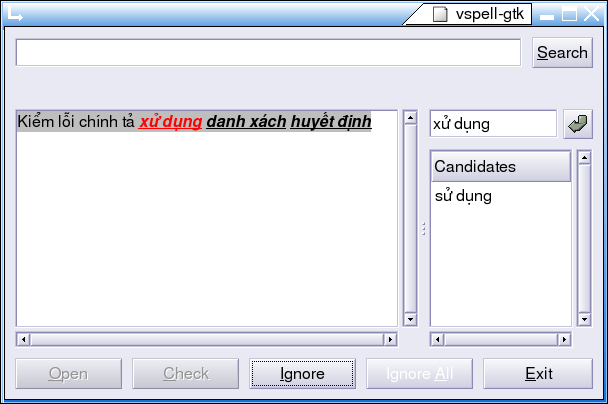
\includegraphics[width=\textwidth]{vspell-gtk}
  \caption{Giao diện vspell-gtk}
  \label{fig:vspell-gtk-ui}
\end{figure}

vspell-gtk tạo lớp \verb@MyText@ dẫn xuất từ \verb@Text@. Các hàm
\verb@ui_syllable_check()@ và \verb@ui_word_check()@ được cài đặt như
trong thuật toán~\vref{algo:MyText::ui_syllable_check}
và~\vref{algo:MyText::ui_word_check}. \verb@MyText@ có thêm vài hàm phụ
để hiển thị như \verb@show_wrong_syllables()@,
\verb@show_wrong_words()@ và \verb@show_words()@.


\begin{algo}
\caption{MyText::ui\_syllable\_check()}
\label{algo:MyText::ui_syllable_check}
\begin{enumerate}
\item Duyệt lần lượt từng tiếng bị sai trong danh sách tiếng sai.
\item Hiện tiếng sai dùng hàm \verb@show_wrong_syllables()@.
\item Lập danh sách tiếng đề nghị dùng
  \verb@get_syllable_candidates()@, hiện thị danh sách tiếng lên màn
  hình.
\item Đặt \verb@processed@, \verb@ignore_all@, \verb@ignore@ là
  \verb@false@. 
\item Lặp liên tục (nhường quyền xử lý cho Gtk+) cho đến khi biến
  \verb@ignore@ hoặc \verb@ignore_all@ hoặc \verb@processed@ là
  \verb@true@. (Khi các nút tương ứng được nhấn, giá trị các biến này
  sẽ bị thay đổi).
\item Nếu \verb@ignore@ là \verb@true@, quay lại từ đầu (chuyển qua từ bị sai
  kế tiếp).
\item Nếu \verb@ignore_all@ là \verb@true@, kết thúc (trả về
  \verb@true@ --- ``sạch lỗi'' do người dùng không muốn kiểm tra lỗi
  tiếng nữa).
\item Nếu \verb@processed@ là \verb@true@.
  \begin{enumerate}
  \item Lấy tiếng do người dùng chọn (hoặc nhập mới).
  \item Thay thế tiếng bị sai trong câu bằng tiếng của người dùng.
  \item Thêm tiếng này vào từ điển tiếng của \verb@VSpell@.
  \item Kết thúc, trả về \verb@false@ --- còn lỗi.
  \end{enumerate}
\end{enumerate}
\end{algo}

\begin{algo}
\caption{MyText::ui\_word\_check()}
\label{algo:MyText::ui_word_check}
\begin{enumerate}
\item Duyệt lần lượt từng từ bị sai trong danh sách từ sai.
\item Hiện từ sai dùng hàm \verb@show_wrong_words()@.
\item Lập danh sách từ đề nghị dùng từ được dùng trong cách tách từ
  đùng khi áp dụng mô hình ngôn ngữ.
%  \verb@get_syllable_candidates()@, hiện thị danh sách tiếng lên màn
%  hình.
\item Đặt \verb@processed@, \verb@ignore_all@, \verb@ignore@ là
  \verb@false@. 
\item Lặp liên tục (nhường quyền xử lý cho Gtk+) cho đến khi biến
  \verb@ignore@ hoặc \verb@ignore_all@ hoặc \verb@processed@ là
  \verb@true@. (Khi các nút tương ứng được nhấn, giá trị các biến này
  sẽ bị thay đổi).
\item Nếu \verb@ignore@ là \verb@true@, quay lại từ đầu (chuyển qua từ bị sai
  kế tiếp).
\item Nếu \verb@ignore_all@ là \verb@true@, kết thúc (trả về
  \verb@true@ --- ``sạch lỗi'' do người dùng không muốn kiểm tra lỗi
  từ nữa).
\item Nếu \verb@processed@ là \verb@true@.
  \begin{enumerate}
  \item Lấy từ do người dùng chọn (hoặc nhập mới).
  \item Tìm ký tự `\verb@|@'. Các ký tự này đại diện cho
    separator. Nếu có, thêm những separator này vào \verb@VSpell@, kết thúc
    --- trả về \verb@false@.
  \item Thay thế từ bị sai trong câu bằng từ của người dùng.
  \item Thêm từ này vào từ điển từ của \verb@VSpell@.
  \item Kết thúc, trả về \verb@false@ --- còn lỗi.
  \end{enumerate}
\end{enumerate}
\end{algo}

\section{Huấn luyện}

\subsection{Dữ liệu huấn luyện}
\label{sec:data-preprocessing}

Dữ liệu gốc bao gồm: danh sách từ và các văn bản tiếng Việt thu thập
từ mạng VnExpress\footnote{http://www.vnexpress.net}.

Nhiệm vụ:
\begin{itemize}
\item Tạo danh sách tiếng, chuẩn hoá danh sách tiếng.
\item Tiền xử lý ngữ liệu.
\item Huấn luyện n\-gram, tạo ra dữ liệu n\-gram.
\end{itemize}


\subsection{Dữ liệu nguồn}
\label{sec:data-source}

Dữ liệu nguồn bao gồm danh sách từ và ngữ liệu tiếng Việt. Dữ liệu
được lưu dưới dạng mã VISCII. 
\subsubsection{Danh sách từ}

Đây là một tập tin văn bản lưu tất cả các từ được dùng trong tiếng
Việt, mỗi từ một dòng. Các chữ cách bởi một khoảng trắng.


\subsubsection{Ngữ liệu huấn luyện}

Bao gồm một loạt các tập tin văn bản tiếng Việt. Mỗi dòng là một đoạn
văn bản.

%% \subsection{Danh sách tiếng}
%% \label{sub:syllable-list}

%% Danh sách tiếng chứa mọi tiếng thông dụng nhất được sử dụng trong
%% tiếng Việt. Danh sách này được rút trích từ danh sách từ, sau đó được
%% lưu ở dạng chuẩn hoá.

%% Danh sách tiếng được rút trích tự động khi chương trình nạp danh sách
%% từ.

%Chương trình syllable-extract được dùng để tạo danh sách này. Cách
%dùng:
%\begin{verbatim}
%$syllable-extract < word-list > syllable-list
%\end{verbatim}


\subsection{Tiền xử lý ngữ liệu huấn luyện}
\label{sec:training-data-preprocessing}

Dữ liệu thu được từ VnExpress bao gồm một loạt các file html, chia
thành nhiều thư mục.

htmltidy được sử dụng để chuyển dữ liệu html về dạng xhtml. Các file
html của VnExpress không hoàn toàn tuân theo chuẩn html, bao gồm hai
trường hợp:

\begin{itemize}
\item Sử dụng tag <vne>
\item Không đóng tag <frame>
\end{itemize}

Hai lỗi này được tự động phát hiện và sửa chữa trước khi chuyển dữ
liệu cho htmltidy.

Sau khi chạy htmltidy, ta được dữ liệu xhtml hợp khuôn dạng. Phân tích
các tài liệu này cho thấy phần nội dung chính thường nằm trong tag
<vne>, hoặc trong tag <table> với thuộc tính id là
``CContainer''. XSLT được sử dụng để lọc ra phần nội dung nằm giữa hai
tag này (\verb#z.xslt#).

Trình \verb#convert.sh# sẽ thực hiện bước htmltidy và xslt ở trên. Cách sử
dụng:
\begin{verbatim}
$convert.sh < input  > output
\end{verbatim}

Sau bước này, ta cần lọc bỏ các tag, loại bỏ các entity~\ldots{}{} để
đưa dữ liệu về dạng văn bản thuần túy. Do số lượng tag được định nghĩa
html rất nhiều nên chỉ xử lý những tag nào được sử dụng trong
VnExpress (thông qua chương trình \verb#gettags.pl#). Các tag này được loại
bỏ bằng \verb#html2text.pl#. Các mã utf-8 được sử dụng trong
VnExpress (thông qua chương trình \verb#z.c#) được chuyển về mã VISCII
qua \verb#z.cpp#. Các entity còn lại (lấy bằng \verb#list-entity.pl#)
được xử lý trong \verb#html2text.pl#.

\verb#html2text.pl# sử dụng các tag để tách dữ liệu thành các đoạn. Dữ
liệu sau cùng là các tập tin văn bản, mỗi dòng là một đoạn.

\subsection{Huấn luyện dữ liệu}
\label{sub:training-data}

Chương trình \verb#wfst-train# được dùng để huấn luyện dữ liệu. Thông
tin nhập là danh sách từ, danh sách tiếng, n\-gram (nếu có). Thông tin
xuất là n\-gram mới.

Quy trình xử lý của trình huấn luyện được nêu trong thuật
toán~\vref{algo:training}. Chương trình được lặp đi lặp lại nhiều lần. 

\begin{algo}
  \caption{Quy trình huấn luyện}
  \label{algo:training}
  \begin{enumerate}
  \item Đọc từng dòng.
  \item Tách câu.
  \item Táck token.
  \item Xây dựng lưới từ (\verb@Lattice::construct()@).
  \item Tìm cách tách từ tốt nhất.
  \item Thống kê n\-gram cho câu.
  \item Xử lý câu kế tiếp.
  \end{enumerate}
\end{algo}

\section{Linh tinh}

\subsection{Xử lý bảng mã}

Chương trình giao tiếp bằng Unicode UTF-8. Tuy nhiên, để tiện việc xử
lý, nội bộ chương trình sử dụng mã VISCII. Do VISCII không thể bao
quát hết Unicode, những ký tự Unicode không có trong VISCII sẽ được
thay bằng một ký tự đặc biệt (coi như là ký tự không biết). Sau khi xử
lý VISCII xong, chuỗi so sánh thật sự sẽ là chuỗi Unicode.

\subsection{So sánh chuỗi}

Do mọi chuỗi đều được lưu thành strid. Việc so sánh chuỗi không phân biệt 
hoa thường là không thể thực hiện được. Do vậy, ngoài strid ``id'' tham chiếu
đến chuỗi gốc, ta sử dụng thêm ``cid'' tham chiếu đến chuỗi được dùng để
so sánh chuỗi. ``cid'' mặc định trong câu tham chiếu đến chuỗi đã
chuẩn hoá. Nếu cần, ``cid'' sẽ tham chiếu đến chuỗi chuẩn hoá, viết
thường.

Khi cần thiết phải so sánh chuỗi thật sự, chương trình sẽ dùng ``id''
để truy ngược đến chuỗi gốc, sau đó thực hiện phép so sánh chuỗi thông thường.

\subsection{Xử lý tiếng Việt}

Một số hàm được tạo ra để hỗ trợ việc xử lý tiếng Việt, bao gồm:
\begin{itemize}
\item \verb@viet_toupper@, \verb@viet_tolower@, \verb@viet_isupper@, \verb@viet_islower@,
  \verb@viet_isalpha@, \verb@viet_isdigit@, \verb@viet_isxdigit@, \verb@viet_isspace@,
  \verb@viet_ispunct@: Các hàm tiếng Việt thay thế cho các hàm gốc (toupper,
  tolower~\ldots)
\item \verb@viet_utf8_to_viscii()@: Chuyển từ UTF-8 sang VISCII. Trả
  về \verb@false@ nếu không thể chuyển đổi.
\item \verb@viet_utf8_to_viscii()@: Chuyển từ UTF-8 sang VISCII. Những
  ký tự không thể chuyển được sẽ được thay bằng `z'.
\item \verb@viet_viscii_to_utf8()@: Chuyển từ VISCII sang UTF-8.
\end{itemize}



\chapter{Đánh giá và kết luận}
\tolerance=200%reset tolerance because i used infinitive tolerance in
              %the last chapter
\label{cha:conclusion}
\minitoc

\section{Tóm tắt}

Sau đây là tóm tắt các đặc điểm mô hình được đề nghị:
\begin{itemize}
\item Áp dụng mô hình tách từ mờ dựa trên n\-gram (bi\-gram và tri\-gram).
\item Cấu trúc dữ liệu dựa trên lưới từ --- một dạng đồ thị có
  hướng không chu trình. Nhờ đó có thể áp dụng thuật toán tìm đường
  trên đồ thị có hướng để tìm ra cách tốt từ tốt nhất.
\item Sử dụng lưới~2-từ cho tri\-gram, các thuật toán làm việc trên
  bi\-gram sẽ vẫn làm việc với tri\-gram thông qua lưới~2-từ.
\item Đồ thị được hiệu chỉnh để tạo
  ra sự khác biệt giữa từ gốc và các từ phát sinh bằng cách điều chỉnh
  giá trị các cạnh nối đến từ phát sinh. 
\item Loại bỏ khả năng cách tách từ
  chứa ít từ hơn có khả năng được chọn cao hơn cách tách từ có nhiều từ
  hơn bằng cách chuẩn hoá các cách tách từ thông qua lưới từ động.
\item Áp dụng đảo ngược lỗi để phục hồi lỗi phát âm và lỗi bàn
  phím. Lỗi bàn phím bao gồm lỗi gõ thiếu phím, dư phím, nhầm phím,
  nhầm thứ tự hai lần gõ. Ngoài ra còn có lỗi do bộ gõ như VNI và
  TELEX.
\item Sử dụng soft-count để huấn luyện n\-gram nhằm tạo ra mô hình ngôn
  ngữ tốt hơn.
\end{itemize}

%% \subsection{Ưu điểm}

%% \begin{itemize}
%% \item 
%% \end{itemize}

\subsection{Hạn chế}

Hạn chế đầu tiên của chương trình chính là lượng thông tin được sử
dụng để khử nhập nhằng khi tách từ mờ. Do chỉ sử dụng thông tin về xác
suất xuất hiện của một chuỗi từ liên tục nên kết quả có phần hạn
chế. Trong nhiều trường hợp ta có thể khử nhập nhằng bằng từ loại,
bằng thông tin cú pháp, hoặc thông tin về ngữ nghĩa. Thông tin xác
suất lẽ ra chỉ là giải pháp bổ trợ cho các thông tin trên. Khi những
thông trên không hoàn chỉnh, không bao quát hết hoặc không thể khử
nhập nhằng toàn bộ, khi đó ta mới dùng thống kê như một giải pháp dự
phòng.

Chính vì chỉ sử dụng n\-gram dựa trên từ, đôi khi chương trình sẽ chọn
lầm cách tách từ, dẫn đến việc thông báo từ sai chính tả trong khi từ
đó hoàn toàn đúng. 

Phần kiểm tra viết hoa khá khó khăn.

%% \begin{itemize}
%% \item Không sử dụng những thông tin cấp cao hơn.
%% \item Có khả năng nó tự động sửa từ đúng thành từ sai, do từ sai
%%   ``hay'' được dùng trong câu đó hơn là từ đúng :-P
%% \end{itemize}

\section{Kết quả thử nghiệm}

Chương trình được huấn luyện dựa trên ngữ liệu từ các bài báo của mạng
VnExpress.net. Ngữ liệu sử dụng có kích thước 12283822 byte, bao gồm
2602105 chữ, khoảng 379000 
câu\footnote{xem phần~\vref{sec:model:sentence-segmentation}  để biết
  các quy tắc tách câu}. Trình huấn luyện chạy trong vòng 13 phút,
trung bình khoảng 485 câu một giây. Dữ
liệu xuất bao gồm 76682 uni\-gram, 446513 bi\-gram, 1101256 tri\-gram với
kích thước tổng cộng 53939974 byte. Mô
hình ngôn ngữ n\-gram-tiếng bao gồm 76224 uni\-gram và 324326 bi\-gram
(8489570 byte). Dữ
liệu tên riêng bao gồm 790 tiếng tạo thành tên người, rút trích từ
7567 tên. Từ điển từ bao gồm 73940 từ, bao gồm 12332 tiếng.

\section{Đánh giá}


\section{Hướng phát triển}
\label{sec:todo}

Do số lượng từ ít, từ ngắn nên lỗi real-word nhiều hơn lỗi non-word --> CSS quan trọng! 

\begin{itemize}
\item Loại bỏ SRILM.
\item Các hướng cải tiến EM.
\item Tư tưởng cơ bản hiện thời là phát sinh mọi trường hợp tương tự
  với trường hợp đang xét và hy vọng giải pháp đúng cũng nằm trong
  đó. Cách này có hai điểm cần bàn:
  \begin{itemize}
  \item Khi nào nên phát sinh, khi nào không? Nói cách khác, khi nào
    ta ``cảm thấy'' chỗ đó có thể bị sai? Statistic/Genetic approach?
  \item Khi phát sinh, nên đánh giá tầm quan trọng của các cách phát
    sinh  cho hợp lý, không nên đánh đồng như hiện nay. How can i do
    that?
  \end{itemize}

  Tách từ không đúng thì bắt lỗi sai. Mà phát sinh quá nhiều thì có
  thể tách từ sẽ sai do có nhiều câu đúng trong đó (giả sử LM hoàn
  hảo). 

  Chuyện phát sinh là chuyện hơi kẹt. Do hiện thời chỉ dựa trên lỗi
  phát âm nên số lượng ít. Nếu áp dụng thêm các lỗi khác (đặc biệt là
  lỗi bàn phím) thì số lượng sẽ tăng đáng kể và {\em xuất hiện những
  câu đúng mới} (giống như việc loại bỏ dấu, sau đó thêm dấu vô sẽ có
  nhiều câu hợp lý). 
  \begin{itemize}
  \item Cách đầu tiên là chỉ phát sinh khi cần thiết ---
    khá khó vì làm sao biết chỗ nào cần phát sinh?
  \item Cách khác là lợi dụng đặc điểm của bắt lỗi chính tả. Khác với
    tách từ thuần túy, lưới từ bắt lỗi chính tả chứa nhiều từ cùng độ
    dài (cùng một ``khuôn''). Làm cách nào đó để nhóm những từ này
    lại, tránh lãng phí khi truy tìm nhiều cách trên cùng một khuôn. 
  \end{itemize}
\item Ngoài cách đang làm, còn hướng nào khác không? Liệu speech
  recognition/OCR có ý kiến nào hay không? Cần tìm hiểu mọi thứ liên
  quan đến ``error tolerance''
\end{itemize}

\section{Khi nào cần phát sinh}

Cách đầu tiên là dựa trên thông tin thống kê, tìm xem giá trị trung
bình của liên kết giữa các từ là bao nhiêu. Nếu liên kết trong lưới từ
thấp hơn ngưỡng này thì phát sinh từ mới.

Áp dụng CSS để phát sinh thêm từ ???

Trước hết, tạo lưới từ cơ sở. Sau đó duyệt qua từng cách tách từ, áp
dụng CSS để tạo thêm một số từ liên quan.
\begin{itemize}
\item Thay thế từ bằng từ do CSS đề nghị --> ảnh hưởng đến CSS ở các
  chỗ khác. Giải pháp genetic hay phân nhánh. Tách làm hai lưới từ
  (một cũ, một mới) sau đó lại áp dụng CSS trên các cách khác ???
\item Thêm vào thay vì thay thế --> ``càng rộng thì càng dễ sai''
\end{itemize}

Chọn đại một cách tách từ, sau đó giao cho CSS. CSS được mở rộng để không
chỉ thay từ, mà thay cả ranh giới từ.

\section{Áp dụng context-sensitive spelling checking}

Các giải pháp spelling checking đều dựa trên câu tách từ sẵn. Xét theo
quan điểm của lưới từ là chọn một đường đi, sau đó áp dụng spelling
checking. Để áp dụng CSS ta có thể đưa nó vô lưới từ thay vì chỉ nằm
trên một đường đi duy nhất trên lưới từ. Nói cách khác, ta chuyển từ
đồ thì ``một đường'' thành một đồ thị đúng nghĩa.

Với các phương pháp sử dụng từ ngữ cảnh, thay vì chỉ xét những từ nằm
trên đường đi, ta xét những từ nằm trên các đường đi khác nhau --
trong một phạm vi nhất định. Khi chọn được một từ thì cũng đồng nghĩa
giới hạn số lưới từ có khả năng lại.

Với các phương pháp dùng collocation, ta cũng có thể mở rộng ra lưới
từ, tìm trên nhiều đường thay vì chỉ một đường.

Vấn đề đối với việc áp dụng những phương pháp này là khả năng ``đoán
sai''. Ví dụ, có một từ trong lưới từ có ảnh hưởng lớn đến quyết định
chọn từ khác. Khi từ đó được sử dụng, nó sẽ loại bỏ các cách tách từ
không chứ nó. Nếu từ đó {\em không} phải là từ đúng thì coi như ta đã
suy luận dựa trên những chứng cớ không đáng tin cậy (độ tin cậy?).

Có thể duyệt từng cách tách từ, áp dụng CSS. Sau đó làm sao biết nên
dùng cách tách từ nào ??? Lại dùng n\-gram?

Túm lại có ba vấn đề:
\begin{itemize}
\item Nếu duyệt từng cách tách từ, số lượng sẽ rất lớn. Cần có cách
  loại bớt những cách tách từ nhảm nhí.
\item Nếu duyệt toàn bộ thì đối với mỗi cách tách từ sẽ có những phát
  hiện lỗi khác nhau. Cần LM hay cái gì đó khác để biết được nên dùng
  cách tách từ nào (hoặc dùng hết :)
\item Cải tiến CSS bằng cách áp dụng lưới từ nhiều hơn, không bị buộc
  trên một đường đi nhất định.
\end{itemize}

\appendix\eject\addcontentsline{toc}{part}{Phụ lục}
\chapter{Dữ liệu thử nghiệm}

\eject\addcontentsline{toc}{chapter}{\listfigurename}\listoffigures
%\refstepcounter{chapter}\addcontentsline{toc}{chapter}{\protect\numberline{\thechapter}\listfigurename}

\eject\addcontentsline{toc}{chapter}{\listtablename}\listoftables
%\refstepcounter{chapter}\addcontentsline{toc}{chapter}{\protect\numberline{\thechapter}\listtablename}

\eject\addcontentsline{toc}{chapter}{Danh sách thuật toán}\listof{algo}{Danh sách thuật toán}
%\refstepcounter{chapter}\addcontentsline{toc}{chapter}{\protect\numberline{\thechapter}Danh sách thuật toán}
%\eject\addcontentsline{toc}{chapter}{\bibname}
\bibliographystyle{alpha}
\bibliography{reference}

%% \begin{thebibliography}{}
%% \bibitem{Ravishankar}Mosur K. Ravishankar. 1996. {\em Efficient Algorithms for
%%   Speech Recognition.} PhD thesis. %CMU-CS-96-143.ps
%% \bibitem{Oflazer}Kemal Oflazer. 1996. {\em Error-tolerant Finite State
%%   Recognition with Applications to Morphological Analysis and Spelling
%%   Correction.} %oflazer96errortolerant.ps.gz
%% \bibitem{LAH}Le An Ha. {\em A method for word segmentation in
%%   Vietnamese.} %Ha-03.pdf
%% \bibitem{Chang}Chao-Huang Chang. {\em A New Approach for
%%   Automatic Chinese Spelling Correction.} %a-new-approach-for.ps
%% \bibitem{Sproat}Richard Sproat, William Gale, Chilin Shih, Nancy
%%   Chang. {\em A Stochastic Finite-State Word-Segmentation Algorithm for
%%   Chinese.} ACL Vol 22 N3.%J96-3004.pdf
%% \bibitem{Chunyu}Chunyu Kit, Zhiming Xu, Jonathan
%%   J. Webster. {\em Integrating N\-Gram Model and Case-based Learning For
%%   Chinese Word Segmentation.}%tsdx.ps.gz
%% \bibitem{softcount}Xianping Ge, Wanda Pratt,
%%   Padhraic Smyth. {\em Discovering Chinese Words from Unsegmented
%%   Text.}%mlwordsigir.ps
%% \bibitem{text-tiling}Jianfeng Gao, Hai-Feng Wang, Mingjing Li, Kai-Fu
%%   Lee. {\em A Unified Approach to Statistical Language Modeling for
%%   Chinese.}%icassp00.pdf
%% \bibitem{}Nianwen Xue.{\em Chinese Word Segmentation as Character
%%   Tagging.}%paper2.pdf
%% \bibitem{self-supervised}Fuchun Peng and Dale Schuurmans. {\em Self-Supervised Chinese
%%   Word Segmentation.}%IDA01.pdf
%% \bibitem{phonetex}Victoria J. Hodge, Jim Austin. {\em An Evaluation of
%%   Phonetic Spell Checkers}%an-evaluation-of-phonetic.ps.gz
%% \bibitem{soundex}K. Kukich. 1992. {\em Techniques for Automatically Correcting
%%   Words in Text.}
%% \bibitem{}Cláudio L. Lucchesi and Tomasz Kowaltowski. {\em Applications of
%%   Finite Automata Representing Large Vocabularies.}%lucchesi92applications.ps.gz
%% \bibitem{}Bo-Hyun Yun, Min-Jeung Cho, Hae-Chang Rim. {\em Segmenting Korean
%%   Compound Nouns using Statistical Information and a Preference
%%   Rule. }%PACLING97.ps 
%% \bibitem{}Roger I. W. Spooner and Alistair D. N. Edwards. {\em User
%%   Modelling for Error Recovery: A Spelling Checker for Dyslexic
%%   Users}%spooner97user.ps.gz 
%% \bibitem{}Theppitak Karoonboonyanan, Virach Sornlertlamvanich,
%%   Surapant Meknavin. {\em A Thai Soundex System for Spelling Correction.}%tsdx.ps.gz
%% \bibitem{}Justin Zobel and Philip Dart. {\em Finding Approximate Matches in
%%   Large Lexicons.}%zobel95finding.ps.gz
%% \bibitem{}Sun Maosong, Shen Dayang, Huang Changning. {\em CSeg\&Tag1.0: A
%%   Practical Word Segmenter and POS Tagger for Chinese Texts.}%A97-1018.pdf
%% \bibitem{wordseg}Đinh Điền, Hoàng Kiếm, Nguyễn Văn Toàn. {\em Vietnamese Word
%%   Segmentation.}%0047-02.pdf
%% \bibitem{}Bidyut Baran Chaudhuri. {\em Reversed word dictionary and
%%   phonetically similar word grouping based spell-checker to Bangla
%%   text.}%bangla.pdf
%% \bibitem{}Timothy Gambell, Charles D. Yang. {\em Scope and Limits of
%%   Statistical Learning in Word Segmentation.}%gambell_yang.pdf
%% \bibitem{iccc}Andi Wu, George Heidorn, Zixin Jiang, Terence
%%   Peng. {\em Correction of Erroneous Characters in Chinese Sentence
%%   Analysis.}%ICCC-2001.pdf
%% \bibitem{}Fuchun Peng, Xiangji Huang, Dale Schuurmans, Shaojun
%%   Wang. {\em Text Clasification in Asian Languages without Word
%%   Segmentation.}%IRAL2003.pdf 
%% \bibitem{}Yalin Wang, Ihsin T. Phillips, Robert
%%   Haralick. {\em Statistical-based Approach to Word Segmentation.}%wordicpr.pdf
%% \bibitem{}{\em Combining Syntactical And Statistical Language Constraints
%%   in Context-dependent Language Models for Interactive Speech
%%   Applications.}%K026.pdf
%% \bibitem{LoiChinhTa}TS. Lê Trung Hoa. 2002. {\em Lỗi chính tả và cách khắc phục. NXB Khoa
%%   học Xã hội.} 
%% \bibitem{LoiTuVung}PGS. Hồ Lê, TS. Trần Thị Ngọc Lang, Tô Đình Nghĩa. 2002. {\em Lỗi từ
%%   vựng và cách khắc phục.} NXB Khoa học Xã hội.
%% \bibitem{Tuoi}PTS. Phan Thị Tươi, KS. Nguyễn Hứa Phùng, KS. Huỳnh Vụ
%%   Như Liên, KS. Phạm Quyết Thắng. 1998. {\em Bắt lỗi chinh tả tự động cho
%%   tiếng Việt bằng máy tính.}
%% \bibitem{worddef}Đinh Điền. 2000. {\em Từ tiếng Việt.} VNU-HCMC.
%% \bibitem{}Andrew R. Golding. 1995. {\em A Bayesian hybrid method for
%%     context-sensitive spelling correction}. Proceedings of the Third
%%     Workshop on Very Large Corpora, pages 39-53.
%% \bibitem{}Andrew R. Golding and Dan Roth. 1999. {\em A Winnow-based
%%     approach to context-sensitive correction}. Machine Learning,
%%     Special issue on Machine Learning and Natural Language Processing,
%%     34:107-130.
%% \bibitem{}Andrew R. Golding and Yves Schabes. 1996. {\em Combining
%%     tri\-gram-based and feature-based methods for context-sensitive
%%     spelling correction}. Proceedings of the 34th Annual Meeting of
%%     the Association for Computational Linguistics.
%% \end{thebibliography}


\end{document}


Giả sử câu S có $n$ tiếng $c_1,c_2,\ldots{},c_n$, có $|S|$ cách tách từ
$S_1,S_2,\ldots{},S_{|S|}$ và cách tách từ  $S_i$ được
tách thành $|S_i|$ từ $W_{i_1},W_{i_2},\ldots{},W_{i_{|S_i|}}$ với 
$W_i$ là một từ xác định bắt đầu ở tiếng thứ $i$ chứa $|W_i|$ tiếng, và
$i_j$ là vị trí từ thứ $j$ trong cách tách câu $i$.

Ta có:
$$p(i)=\sum_{j=1}^{|S_i|}{p(W_{i_j})}$$

Một câu sẽ được tách thành:
$$P(W_i) = P_{i}^{left}p(W_{i})P_{i+|W_i|}^{right}$$

$P_i^{left}$ là xác suất tất cả các tổ hợp từ có thể có từ 
tiếng thứ nhất đến tiếng thứ $i$.

$P_{i}^{right}$ là xác suất tất cả các tổ hợp từ có thể có từ tiếng
thứ  $i$ đến hết câu. 

Dễ thấy, với mỗi từ $C$ trong câu $S$, fractional count W của từ sẽ là
$\displaystyle\frac{P(W)}{\sum_i^{|S|}p(i)}$.

$\displaystyle\sum_i^{|S|}p(i)$ cũng chính là $P_{n+1}^{left}$ theo
định nghĩa $P_i^{left}$.

Ta sẽ dùng quy hoạch động để tính $P_i^{left}$ và $P_i^{right}$

$$
P_i^{left} = \left\{
  \begin{array}{lr}
    1 & i=1\\
    p(W_i) & i=2\\
    \sum_{j=1}^{i-1}p(c_j\ldots{} c_{i-1})P_j^{left} & i>2
  \end{array}
\right.
$$

$$
p(c_i\ldots{} c_j) = \left\{
  \begin{array}{ll}
    p(W_i)&\text{nếu } c_i\ldots{} c_j \text{ tạo thành } W_i\\
    0&\text{ngược lại}
  \end{array}
\right.
$$

Thuật toán tính $P^{left}$ như sau:
\begin{enumerate}
\item Đặt $P_1^{left} = 1$
\item Đặt $P_i^{left} = 0\quad \forall i \in [2\ldots{} n+1]$
\item Duyệt i từ 1 đến n, tìm tất cả các từ $W_i$ (do tại có thể có
  nhiều từ bắt đầu tại tiếng $i$).
  Với mỗi từ $W_i$ tìm được, cộng thêm $p(W_i)$ vào $P_{i+|W_i|}^{left}$
\end{enumerate}

Thuật toán tương tự được áp dụng để tính $P^{right}$.

Sau khi tính được $P^{left}$ và $P^{right}$, ta có thể tính fractional
count trong câu bằng cách duyệt tất cả các từ có thể có trong câu,
cộng thêm vào $\displaystyle\frac{P(W)}{P_{n+1}^{left}}$ cho từ
$C$. Thực tế, ta sẽ lồng bước này vào trong thuật toán tính
$P^{right}$, vì thuật toán cũng phải duyệt qua tất cả các từ.

Vậy thuật toán tính $P^{right}$ là:
\begin{enumerate}
\item Đặt $P_{n+1}^{right} = 1$
\item Đặt $P_i^{right} = 0\quad \forall i \in [1\ldots{} n]$
\item Duyệt i từ n+1 đến 1.
  \begin{enumerate}
  \item tìm tất cả các từ $W_j$ sao cho $j+|W_j|=i$.
    Với mỗi từ $W_j$ tìm được, cộng thêm $p(W_j)$ vào
    $P_j^{right}$
  \item Tính fractional count cho tất cả các từ $W_i$ ($i \le n$)
  \end{enumerate}
\end{enumerate}


Ví dụ: câu ``học sinh học sinh học'' có 8 cách tách từ
\begin{verbatim}
học-sinh học-sinh học
học-sinh học sinh học
học-sinh học sinh-học
học sinh học sinh học
học sinh học sinh-học
học sinh học-sinh học
học sinh-học sinh học
học sinh-học sinh-học
\end{verbatim}
\def\Zhs{\text{học-sinh}}
\def\Zsh{\text{sinh-học}}
\def\Zh{\text{học}}
\def\Zs{\text{sinh}}
Ta có
$$
\begin{array}{rl}
P_1^{left}(\Zhs) &= p(\Zhs_1/\phi)\\
P_1^{left}(\Zh) &= p(\Zh_1/\phi)\\
P_2^{left}(\Zs) &= p(\Zs_2/\Zh_1)P_1^{left}(\Zh)\\
 &=p(\Zs_2/\Zh_1)p(\Zh_1/\phi)\\
P_2^{left}(\Zsh) &= p(\Zsh_2/\Zh_1)P_1^{left}(\Zh)\\
 &=p(\Zsh_2/\Zh_1)p(\Zh_1/\phi)\\
P_3^{left}(\Zhs) &= p(\Zhs_3/\Zhs_1)P_1^{left}(\Zhs)+p(\Zhs_3/\Zs_2)P_2^{left}(\Zs)\\
 &=p(\Zhs_3/\Zhs_1)p(\Zhs_1/\phi)+p(\Zhs_3/\Zs_2)p(\Zs_2/\Zh_1)p(\Zh_1/\phi)\\
 &=p(\Zhs_1,\Zhs_3)+p(\Zh_1,\Zs_2,\Zhs_3)\\
P_3^{left}(\Zh) &= p(\Zh_3/\Zs_2)P_2^{left}(\Zs)+p(\Zh_3/\Zhs_1)P_1^{left}(\Zhs)\\
 &=p(\Zh_3/\Zs_2)p(\Zs_2/\Zh_1)p(\Zh_1/\phi)+p(\Zh_3/\Zhs_1)p(\Zhs_1/\phi)\\
 &=p(\Zh_1,\Zs_2,\Zh_3)+p(\Zhs_1,\Zh_3)\\
\end{array}
$$

$$
\begin{array}{rl}
P_5^{right}(\Zh) &= p(\Phi/\Zh_5)\\
P_4^{right}(\Zsh) &= p(\Phi/\Zsh_4)\\
P_4^{right}(\Zs) &= p(\Zh_5/\Zs_4)P_5^{right}(\Zh)\\
 &=p(\Zh_5/\Zs_4)p(\Phi/\Zh_5)\\
P_3^{right}(\Zh) &= p(\Zsh_4/\Zh_3)P_4^{right}(\Zsh)+p(\Zs_4/\Zh_3)P_4^{right}(\Zs)\\
 &=p(\Zsh_4/\Zh_3)p(\Phi/\Zsh_4)+p(\Zs_4/\Zh_3)(\Zh_5/\Zs_4)p(\Phi/\Zh_5)\\
 &=p(\Zh_3,\Zsh_4)+p(\Zh_3,\Zs_4,\Zh_5)\\
P_3^{right}(\Zhs) &= p(\Zh_5/\Zhs_3)P_5^{right}(\Zh)\\
 &=p(\Zh_5/\Zhs_3)p(\Phi/\Zh_5)\\
 &=p(\Zhs_3,\Zh_5)\\
\end{array}
$$

$$
\begin{array}{rl}
P_3(\Zhs) &= P_3^{left}(\Zhs)P_3^{right}(\Zhs)\\
 &=[p(\Zhs_1,\Zhs_3)+p(\Zh_1,\Zs_2,\Zhs_3)]p(\Zhs_3,\Zh_5)\\
 &=p(\Zhs_1,\Zhs_3)p(\Zhs_3,\Zh_5)+p(\Zh_1,\Zs_2,\Zhs_3)p(\Zhs_3,\Zh_5)\\
 &=p(\Zhs_1,\Zhs_3,\Zh_5)+p(\Zh_1,\Zs_2,\Zhs_3,\Zh_5)
\end{array}
$$


Với \cite{Tuoi} thì việc xử lý lỗi bao gồm:
\begin{itemize}
\item Từ không có trong từ điển thì bắt lỗi ở cấp từ vựng.
\item Từ có trong từ điển thị bắt lỗi ở cấp cú pháp.
\end{itemize}

